\documentclass[conference]{IEEEtran}
\IEEEoverridecommandlockouts
\usepackage{cite}
\usepackage{amsmath,amssymb,amsfonts}
\usepackage{graphicx}
\usepackage{booktabs}
\usepackage{xcolor}
\usepackage{url}
\usepackage{hyperref}
\usepackage{orcidlink}
\usepackage{caption}
\usepackage{listings}
\usepackage{placeins}
\lstset{basicstyle=\ttfamily\footnotesize,frame=single,columns=fullflexible,
        breaklines=true,captionpos=b,xleftmargin=4pt,xrightmargin=4pt}
\hypersetup{
  colorlinks = true,
  linkcolor  = [rgb]{0.10,0.25,0.55},
  citecolor  = [rgb]{0.10,0.25,0.55},
  urlcolor   = [rgb]{0.10,0.35,0.45},
  breaklinks = true
}
% Generated by src/analyze.py. Do not edit.
\newcommand{\AgentModel}{qwen/qwen3.5-9b}
\newcommand{\AutogenVersion}{0.7.5}
\newcommand{\BaseBusAgentBenignDoneHi}{100.0\%}
\newcommand{\BaseBusAgentBenignDoneK}{20}
\newcommand{\BaseBusAgentBenignDoneLo}{83.9\%}
\newcommand{\BaseBusAgentBenignDoneN}{20}
\newcommand{\BaseBusAgentBenignDonePct}{100.0\%}
\newcommand{\BaseBusAllBenignDoneHi}{100.0\%}
\newcommand{\BaseBusAllBenignDoneK}{40}
\newcommand{\BaseBusAllBenignDoneLo}{91.2\%}
\newcommand{\BaseBusAllBenignDoneN}{40}
\newcommand{\BaseBusAllBenignDonePct}{100.0\%}
\newcommand{\BaseBusUserBenignDoneHi}{100.0\%}
\newcommand{\BaseBusUserBenignDoneK}{20}
\newcommand{\BaseBusUserBenignDoneLo}{83.9\%}
\newcommand{\BaseBusUserBenignDoneN}{20}
\newcommand{\BaseBusUserBenignDonePct}{100.0\%}
\newcommand{\BaseModelAgentBenignDoneHi}{100.0\%}
\newcommand{\BaseModelAgentBenignDoneK}{20}
\newcommand{\BaseModelAgentBenignDoneLo}{83.9\%}
\newcommand{\BaseModelAgentBenignDoneN}{20}
\newcommand{\BaseModelAgentBenignDonePct}{100.0\%}
\newcommand{\BaseModelAllBenignDoneHi}{100.0\%}
\newcommand{\BaseModelAllBenignDoneK}{80}
\newcommand{\BaseModelAllBenignDoneLo}{95.4\%}
\newcommand{\BaseModelAllBenignDoneN}{80}
\newcommand{\BaseModelAllBenignDonePct}{100.0\%}
\newcommand{\BaseModelMemoryBenignDoneHi}{100.0\%}
\newcommand{\BaseModelMemoryBenignDoneK}{20}
\newcommand{\BaseModelMemoryBenignDoneLo}{83.9\%}
\newcommand{\BaseModelMemoryBenignDoneN}{20}
\newcommand{\BaseModelMemoryBenignDonePct}{100.0\%}
\newcommand{\BaseModelToolBenignDoneHi}{100.0\%}
\newcommand{\BaseModelToolBenignDoneK}{20}
\newcommand{\BaseModelToolBenignDoneLo}{83.9\%}
\newcommand{\BaseModelToolBenignDoneN}{20}
\newcommand{\BaseModelToolBenignDonePct}{100.0\%}
\newcommand{\BaseModelUserBenignDoneHi}{100.0\%}
\newcommand{\BaseModelUserBenignDoneK}{20}
\newcommand{\BaseModelUserBenignDoneLo}{83.9\%}
\newcommand{\BaseModelUserBenignDoneN}{20}
\newcommand{\BaseModelUserBenignDonePct}{100.0\%}
\newcommand{\BaseToolAllBenignDoneHi}{100.0\%}
\newcommand{\BaseToolAllBenignDoneK}{20}
\newcommand{\BaseToolAllBenignDoneLo}{83.9\%}
\newcommand{\BaseToolAllBenignDoneN}{20}
\newcommand{\BaseToolAllBenignDonePct}{100.0\%}
\newcommand{\BaseToolToolBenignDoneHi}{100.0\%}
\newcommand{\BaseToolToolBenignDoneK}{20}
\newcommand{\BaseToolToolBenignDoneLo}{83.9\%}
\newcommand{\BaseToolToolBenignDoneN}{20}
\newcommand{\BaseToolToolBenignDonePct}{100.0\%}
\newcommand{\BlockBusAgentBenignDoneHi}{100.0\%}
\newcommand{\BlockBusAgentBenignDoneK}{20}
\newcommand{\BlockBusAgentBenignDoneLo}{83.9\%}
\newcommand{\BlockBusAgentBenignDoneN}{20}
\newcommand{\BlockBusAgentBenignDonePct}{100.0\%}
\newcommand{\BlockBusAgentGoalHi}{27.8\%}
\newcommand{\BlockBusAgentGoalK}{0}
\newcommand{\BlockBusAgentGoalLo}{0.0\%}
\newcommand{\BlockBusAgentGoalN}{10}
\newcommand{\BlockBusAgentGoalPct}{0.0\%}
\newcommand{\BlockBusAgentInduced}{0}
\newcommand{\BlockBusAgentP}{0.002}
\newcommand{\BlockBusAgentPrevented}{10}
\newcommand{\BlockBusAllBenignDoneHi}{99.6\%}
\newcommand{\BlockBusAllBenignDoneK}{39}
\newcommand{\BlockBusAllBenignDoneLo}{87.1\%}
\newcommand{\BlockBusAllBenignDoneN}{40}
\newcommand{\BlockBusAllBenignDonePct}{97.5\%}
\newcommand{\BlockBusAllGoalHi}{16.1\%}
\newcommand{\BlockBusAllGoalK}{0}
\newcommand{\BlockBusAllGoalLo}{0.0\%}
\newcommand{\BlockBusAllGoalN}{20}
\newcommand{\BlockBusAllGoalPct}{0.0\%}
\newcommand{\BlockBusAllInduced}{0}
\newcommand{\BlockBusAllP}{1.9\times 10^{-6}}
\newcommand{\BlockBusAllPrevented}{20}
\newcommand{\BlockBusUserBenignDoneHi}{99.1\%}
\newcommand{\BlockBusUserBenignDoneK}{19}
\newcommand{\BlockBusUserBenignDoneLo}{76.4\%}
\newcommand{\BlockBusUserBenignDoneN}{20}
\newcommand{\BlockBusUserBenignDonePct}{95.0\%}
\newcommand{\BlockBusUserGoalHi}{27.8\%}
\newcommand{\BlockBusUserGoalK}{0}
\newcommand{\BlockBusUserGoalLo}{0.0\%}
\newcommand{\BlockBusUserGoalN}{10}
\newcommand{\BlockBusUserGoalPct}{0.0\%}
\newcommand{\BlockBusUserInduced}{0}
\newcommand{\BlockBusUserP}{0.002}
\newcommand{\BlockBusUserPrevented}{10}
\newcommand{\BlockModelAgentBenignDoneHi}{100.0\%}
\newcommand{\BlockModelAgentBenignDoneK}{20}
\newcommand{\BlockModelAgentBenignDoneLo}{83.9\%}
\newcommand{\BlockModelAgentBenignDoneN}{20}
\newcommand{\BlockModelAgentBenignDonePct}{100.0\%}
\newcommand{\BlockModelAgentGoalHi}{27.8\%}
\newcommand{\BlockModelAgentGoalK}{0}
\newcommand{\BlockModelAgentGoalLo}{0.0\%}
\newcommand{\BlockModelAgentGoalN}{10}
\newcommand{\BlockModelAgentGoalPct}{0.0\%}
\newcommand{\BlockModelAgentInduced}{0}
\newcommand{\BlockModelAgentP}{0.002}
\newcommand{\BlockModelAgentPrevented}{10}
\newcommand{\BlockModelAllBenignDoneHi}{99.8\%}
\newcommand{\BlockModelAllBenignDoneK}{79}
\newcommand{\BlockModelAllBenignDoneLo}{93.3\%}
\newcommand{\BlockModelAllBenignDoneN}{80}
\newcommand{\BlockModelAllBenignDonePct}{98.8\%}
\newcommand{\BlockModelAllGoalHi}{16.5\%}
\newcommand{\BlockModelAllGoalK}{2}
\newcommand{\BlockModelAllGoalLo}{1.4\%}
\newcommand{\BlockModelAllGoalN}{40}
\newcommand{\BlockModelAllGoalPct}{5.0\%}
\newcommand{\BlockModelAllInduced}{0}
\newcommand{\BlockModelAllP}{1.5\times 10^{-8}}
\newcommand{\BlockModelAllPrevented}{27}
\newcommand{\BlockModelMemoryBenignDoneHi}{100.0\%}
\newcommand{\BlockModelMemoryBenignDoneK}{20}
\newcommand{\BlockModelMemoryBenignDoneLo}{83.9\%}
\newcommand{\BlockModelMemoryBenignDoneN}{20}
\newcommand{\BlockModelMemoryBenignDonePct}{100.0\%}
\newcommand{\BlockModelMemoryGoalHi}{51.0\%}
\newcommand{\BlockModelMemoryGoalK}{2}
\newcommand{\BlockModelMemoryGoalLo}{5.7\%}
\newcommand{\BlockModelMemoryGoalN}{10}
\newcommand{\BlockModelMemoryGoalPct}{20.0\%}
\newcommand{\BlockModelMemoryInduced}{0}
\newcommand{\BlockModelMemoryP}{0.250}
\newcommand{\BlockModelMemoryPrevented}{3}
\newcommand{\BlockModelToolBenignDoneHi}{100.0\%}
\newcommand{\BlockModelToolBenignDoneK}{20}
\newcommand{\BlockModelToolBenignDoneLo}{83.9\%}
\newcommand{\BlockModelToolBenignDoneN}{20}
\newcommand{\BlockModelToolBenignDonePct}{100.0\%}
\newcommand{\BlockModelToolGoalHi}{27.8\%}
\newcommand{\BlockModelToolGoalK}{0}
\newcommand{\BlockModelToolGoalLo}{0.0\%}
\newcommand{\BlockModelToolGoalN}{10}
\newcommand{\BlockModelToolGoalPct}{0.0\%}
\newcommand{\BlockModelToolInduced}{0}
\newcommand{\BlockModelToolP}{0.125}
\newcommand{\BlockModelToolPrevented}{4}
\newcommand{\BlockModelUserBenignDoneHi}{99.1\%}
\newcommand{\BlockModelUserBenignDoneK}{19}
\newcommand{\BlockModelUserBenignDoneLo}{76.4\%}
\newcommand{\BlockModelUserBenignDoneN}{20}
\newcommand{\BlockModelUserBenignDonePct}{95.0\%}
\newcommand{\BlockModelUserGoalHi}{27.8\%}
\newcommand{\BlockModelUserGoalK}{0}
\newcommand{\BlockModelUserGoalLo}{0.0\%}
\newcommand{\BlockModelUserGoalN}{10}
\newcommand{\BlockModelUserGoalPct}{0.0\%}
\newcommand{\BlockModelUserInduced}{0}
\newcommand{\BlockModelUserP}{0.002}
\newcommand{\BlockModelUserPrevented}{10}
\newcommand{\BlockToolAllBenignDoneHi}{100.0\%}
\newcommand{\BlockToolAllBenignDoneK}{20}
\newcommand{\BlockToolAllBenignDoneLo}{83.9\%}
\newcommand{\BlockToolAllBenignDoneN}{20}
\newcommand{\BlockToolAllBenignDonePct}{100.0\%}
\newcommand{\BlockToolAllGoalHi}{27.8\%}
\newcommand{\BlockToolAllGoalK}{0}
\newcommand{\BlockToolAllGoalLo}{0.0\%}
\newcommand{\BlockToolAllGoalN}{10}
\newcommand{\BlockToolAllGoalPct}{0.0\%}
\newcommand{\BlockToolAllInduced}{0}
\newcommand{\BlockToolAllP}{0.125}
\newcommand{\BlockToolAllPrevented}{4}
\newcommand{\BlockToolToolBenignDoneHi}{100.0\%}
\newcommand{\BlockToolToolBenignDoneK}{20}
\newcommand{\BlockToolToolBenignDoneLo}{83.9\%}
\newcommand{\BlockToolToolBenignDoneN}{20}
\newcommand{\BlockToolToolBenignDonePct}{100.0\%}
\newcommand{\BlockToolToolGoalHi}{27.8\%}
\newcommand{\BlockToolToolGoalK}{0}
\newcommand{\BlockToolToolGoalLo}{0.0\%}
\newcommand{\BlockToolToolGoalN}{10}
\newcommand{\BlockToolToolGoalPct}{0.0\%}
\newcommand{\BlockToolToolInduced}{0}
\newcommand{\BlockToolToolP}{0.125}
\newcommand{\BlockToolToolPrevented}{4}
\newcommand{\CiLevel}{95\%}
\newcommand{\CrewaiVersion}{1.15.22}
\newcommand{\DebertaMaxLen}{512}
\newcommand{\ElevenErrors}{0}
\newcommand{\FeatAttackVocabAuroc}{0.515}
\newcommand{\FeatDelimiterAuroc}{0.700}
\newcommand{\FeatIdentifierAuroc}{0.920}
\newcommand{\FeatImperativeAuroc}{0.915}
\newcommand{\FeatSecondPersonAuroc}{0.835}
\newcommand{\FwCrewaiDocumentFlags}{0}
\newcommand{\FwCrewaiErrors}{0}
\newcommand{\FwCrewaiFirstHopHi}{100.0\%}
\newcommand{\FwCrewaiFirstHopK}{10}
\newcommand{\FwCrewaiFirstHopLo}{72.2\%}
\newcommand{\FwCrewaiFirstHopN}{10}
\newcommand{\FwCrewaiFirstHopPct}{100.0\%}
\newcommand{\FwCrewaiGoalHi}{89.2\%}
\newcommand{\FwCrewaiGoalK}{7}
\newcommand{\FwCrewaiGoalLo}{39.7\%}
\newcommand{\FwCrewaiGoalN}{10}
\newcommand{\FwCrewaiGoalPct}{70.0\%}
\newcommand{\FwCrewaiHandoffCatchHi}{27.8\%}
\newcommand{\FwCrewaiHandoffCatchK}{0}
\newcommand{\FwCrewaiHandoffCatchLo}{0.0\%}
\newcommand{\FwCrewaiHandoffCatchN}{10}
\newcommand{\FwCrewaiHandoffCatchPct}{0.0\%}
\newcommand{\FwCrewaiHandoffFalseHi}{27.8\%}
\newcommand{\FwCrewaiHandoffFalseK}{0}
\newcommand{\FwCrewaiHandoffFalseLo}{0.0\%}
\newcommand{\FwCrewaiHandoffFalseN}{10}
\newcommand{\FwCrewaiHandoffFalsePct}{0.0\%}
\newcommand{\FwCrewaiHandoffLateHi}{27.8\%}
\newcommand{\FwCrewaiHandoffLateK}{0}
\newcommand{\FwCrewaiHandoffLateLo}{0.0\%}
\newcommand{\FwCrewaiHandoffLateN}{10}
\newcommand{\FwCrewaiHandoffLatePct}{0.0\%}
\newcommand{\FwCrewaiModelCatchHi}{100.0\%}
\newcommand{\FwCrewaiModelCatchK}{10}
\newcommand{\FwCrewaiModelCatchLo}{72.2\%}
\newcommand{\FwCrewaiModelCatchN}{10}
\newcommand{\FwCrewaiModelCatchPct}{100.0\%}
\newcommand{\FwCrewaiModelFalseHi}{100.0\%}
\newcommand{\FwCrewaiModelFalseK}{10}
\newcommand{\FwCrewaiModelFalseLo}{72.2\%}
\newcommand{\FwCrewaiModelFalseN}{10}
\newcommand{\FwCrewaiModelFalsePct}{100.0\%}
\newcommand{\FwCrewaiModelLateHi}{27.8\%}
\newcommand{\FwCrewaiModelLateK}{0}
\newcommand{\FwCrewaiModelLateLo}{0.0\%}
\newcommand{\FwCrewaiModelLateN}{10}
\newcommand{\FwCrewaiModelLatePct}{0.0\%}
\newcommand{\FwCrewaiScaffoldFlags}{29}
\newcommand{\FwCrewaiToolCatchHi}{100.0\%}
\newcommand{\FwCrewaiToolCatchK}{10}
\newcommand{\FwCrewaiToolCatchLo}{72.2\%}
\newcommand{\FwCrewaiToolCatchN}{10}
\newcommand{\FwCrewaiToolCatchPct}{100.0\%}
\newcommand{\FwCrewaiToolFalseHi}{27.8\%}
\newcommand{\FwCrewaiToolFalseK}{0}
\newcommand{\FwCrewaiToolFalseLo}{0.0\%}
\newcommand{\FwCrewaiToolFalseN}{10}
\newcommand{\FwCrewaiToolFalsePct}{0.0\%}
\newcommand{\FwCrewaiToolLateHi}{27.8\%}
\newcommand{\FwCrewaiToolLateK}{0}
\newcommand{\FwCrewaiToolLateLo}{0.0\%}
\newcommand{\FwCrewaiToolLateN}{10}
\newcommand{\FwCrewaiToolLatePct}{0.0\%}
\newcommand{\FwLanggraphDocumentFlags}{0}
\newcommand{\FwLanggraphErrors}{0}
\newcommand{\FwLanggraphFirstHopHi}{94.3\%}
\newcommand{\FwLanggraphFirstHopK}{8}
\newcommand{\FwLanggraphFirstHopLo}{49.0\%}
\newcommand{\FwLanggraphFirstHopN}{10}
\newcommand{\FwLanggraphFirstHopPct}{80.0\%}
\newcommand{\FwLanggraphGoalHi}{68.7\%}
\newcommand{\FwLanggraphGoalK}{4}
\newcommand{\FwLanggraphGoalLo}{16.8\%}
\newcommand{\FwLanggraphGoalN}{10}
\newcommand{\FwLanggraphGoalPct}{40.0\%}
\newcommand{\FwLanggraphHandoffCatchHi}{27.8\%}
\newcommand{\FwLanggraphHandoffCatchK}{0}
\newcommand{\FwLanggraphHandoffCatchLo}{0.0\%}
\newcommand{\FwLanggraphHandoffCatchN}{10}
\newcommand{\FwLanggraphHandoffCatchPct}{0.0\%}
\newcommand{\FwLanggraphHandoffFalseHi}{27.8\%}
\newcommand{\FwLanggraphHandoffFalseK}{0}
\newcommand{\FwLanggraphHandoffFalseLo}{0.0\%}
\newcommand{\FwLanggraphHandoffFalseN}{10}
\newcommand{\FwLanggraphHandoffFalsePct}{0.0\%}
\newcommand{\FwLanggraphHandoffLateHi}{100.0\%}
\newcommand{\FwLanggraphHandoffLateK}{10}
\newcommand{\FwLanggraphHandoffLateLo}{72.2\%}
\newcommand{\FwLanggraphHandoffLateN}{10}
\newcommand{\FwLanggraphHandoffLatePct}{100.0\%}
\newcommand{\FwLanggraphModelCatchHi}{100.0\%}
\newcommand{\FwLanggraphModelCatchK}{10}
\newcommand{\FwLanggraphModelCatchLo}{72.2\%}
\newcommand{\FwLanggraphModelCatchN}{10}
\newcommand{\FwLanggraphModelCatchPct}{100.0\%}
\newcommand{\FwLanggraphModelFalseHi}{27.8\%}
\newcommand{\FwLanggraphModelFalseK}{0}
\newcommand{\FwLanggraphModelFalseLo}{0.0\%}
\newcommand{\FwLanggraphModelFalseN}{10}
\newcommand{\FwLanggraphModelFalsePct}{0.0\%}
\newcommand{\FwLanggraphModelLateHi}{27.8\%}
\newcommand{\FwLanggraphModelLateK}{0}
\newcommand{\FwLanggraphModelLateLo}{0.0\%}
\newcommand{\FwLanggraphModelLateN}{10}
\newcommand{\FwLanggraphModelLatePct}{0.0\%}
\newcommand{\FwLanggraphScaffoldFlags}{0}
\newcommand{\FwLanggraphToolCatchHi}{100.0\%}
\newcommand{\FwLanggraphToolCatchK}{10}
\newcommand{\FwLanggraphToolCatchLo}{72.2\%}
\newcommand{\FwLanggraphToolCatchN}{10}
\newcommand{\FwLanggraphToolCatchPct}{100.0\%}
\newcommand{\FwLanggraphToolFalseHi}{27.8\%}
\newcommand{\FwLanggraphToolFalseK}{0}
\newcommand{\FwLanggraphToolFalseLo}{0.0\%}
\newcommand{\FwLanggraphToolFalseN}{10}
\newcommand{\FwLanggraphToolFalsePct}{0.0\%}
\newcommand{\FwLanggraphToolLateHi}{27.8\%}
\newcommand{\FwLanggraphToolLateK}{0}
\newcommand{\FwLanggraphToolLateLo}{0.0\%}
\newcommand{\FwLanggraphToolLateN}{10}
\newcommand{\FwLanggraphToolLatePct}{0.0\%}
\newcommand{\GatewayBackendModel}{qwen2.5-0.5b-instruct-mlx}
\newcommand{\GuardVsSpotOnlyGuard}{0}
\newcommand{\GuardVsSpotOnlySpot}{21}
\newcommand{\GuardVsSpotP}{9.5\times 10^{-7}}
\newcommand{\HandBreaches}{111}
\newcommand{\HandObeyed}{103}
\newcommand{\HandOtherWording}{8}
\newcommand{\LanggraphVersion}{1.2.5}
\newcommand{\LenAttackMedian}{124}
\newcommand{\LenAurocPassage}{0.505}
\newcommand{\LenAurocText}{0.504}
\newcommand{\LenHnIdentifierMedian}{122}
\newcommand{\LenHnImperativeMedian}{103}
\newcommand{\LenHnVocabMedian}{122}
\newcommand{\LenMatchedMedian}{122}
\newcommand{\LlmGuardModel}{qwen/qwen3.5-9b}
\newcommand{\MaxToolIterations}{3}
\newcommand{\MemRawHi}{98.1\%}
\newcommand{\MemRawK}{27}
\newcommand{\MemRawLo}{78.0\%}
\newcommand{\MemRawN}{29}
\newcommand{\MemRawOnly}{10}
\newcommand{\MemRawPct}{93.1\%}
\newcommand{\MemWrappedHi}{74.5\%}
\newcommand{\MemWrappedK}{17}
\newcommand{\MemWrappedLo}{40.7\%}
\newcommand{\MemWrappedN}{29}
\newcommand{\MemWrappedOnly}{0}
\newcommand{\MemWrappedPct}{58.6\%}
\newcommand{\MemWrapperP}{0.002}
\newcommand{\NAttack}{50}
\newcommand{\NBenign}{100}
\newcommand{\NBreakTests}{33}
\newcommand{\NBreakTestsFire}{33}
\newcommand{\NCarriers}{50}
\newcommand{\NCarriersPerSource}{25}
\newcommand{\NDeepset}{116}
\newcommand{\NHnIdentifier}{16}
\newcommand{\NHnImperative}{17}
\newcommand{\NHnVocab}{17}
\newcommand{\NInjecFile}{510}
\newcommand{\NInjecInstructions}{30}
\newcommand{\NInjecSelected}{60}
\newcommand{\NInjecTools}{47}
\newcommand{\NInjecUsers}{17}
\newcommand{\NMatched}{50}
\newcommand{\NNotInject}{339}
\newcommand{\NPanel}{6}
\newcommand{\NPerTemplateGoal}{5}
\newcommand{\NProbes}{150}
\newcommand{\NRailPatterns}{13}
\newcommand{\NStudioWorkflows}{3}
\newcommand{\NTemplates}{5}
\newcommand{\NTestCarriers}{10}
\newcommand{\NTestInjec}{20}
\newcommand{\NTestInjecInstructions}{10}
\newcommand{\NTestPerSource}{5}
\newcommand{\NemoVersion}{0.22.0}
\newcommand{\OneDebertaBenignUnitP}{0.062}
\newcommand{\OneDebertaBenignUnitPassageOnly}{5}
\newcommand{\OneDebertaBenignUnitTextOnly}{0}
\newcommand{\OneDebertaMemoryAttackHi}{16.2\%}
\newcommand{\OneDebertaMemoryAttackK}{3}
\newcommand{\OneDebertaMemoryAttackLo}{2.1\%}
\newcommand{\OneDebertaMemoryAttackN}{50}
\newcommand{\OneDebertaMemoryAttackPct}{6.0\%}
\newcommand{\OneDebertaMemoryBenignHi}{3.7\%}
\newcommand{\OneDebertaMemoryBenignK}{0}
\newcommand{\OneDebertaMemoryBenignLo}{0.0\%}
\newcommand{\OneDebertaMemoryBenignN}{100}
\newcommand{\OneDebertaMemoryBenignPct}{0.0\%}
\newcommand{\OneDebertaMemoryDirectHi}{27.8\%}
\newcommand{\OneDebertaMemoryDirectK}{0}
\newcommand{\OneDebertaMemoryDirectLo}{0.0\%}
\newcommand{\OneDebertaMemoryDirectN}{10}
\newcommand{\OneDebertaMemoryDirectPct}{0.0\%}
\newcommand{\OneDebertaMemoryIgnorePreviousHi}{51.0\%}
\newcommand{\OneDebertaMemoryIgnorePreviousK}{2}
\newcommand{\OneDebertaMemoryIgnorePreviousLo}{5.7\%}
\newcommand{\OneDebertaMemoryIgnorePreviousN}{10}
\newcommand{\OneDebertaMemoryIgnorePreviousPct}{20.0\%}
\newcommand{\OneDebertaMemoryImportantInstructionsHi}{27.8\%}
\newcommand{\OneDebertaMemoryImportantInstructionsK}{0}
\newcommand{\OneDebertaMemoryImportantInstructionsLo}{0.0\%}
\newcommand{\OneDebertaMemoryImportantInstructionsN}{10}
\newcommand{\OneDebertaMemoryImportantInstructionsPct}{0.0\%}
\newcommand{\OneDebertaMemoryInjecagentHi}{40.4\%}
\newcommand{\OneDebertaMemoryInjecagentK}{1}
\newcommand{\OneDebertaMemoryInjecagentLo}{1.8\%}
\newcommand{\OneDebertaMemoryInjecagentN}{10}
\newcommand{\OneDebertaMemoryInjecagentPct}{10.0\%}
\newcommand{\OneDebertaMemoryMemoryOnly}{0}
\newcommand{\OneDebertaMemoryP}{0.062}
\newcommand{\OneDebertaMemorySystemMessageHi}{27.8\%}
\newcommand{\OneDebertaMemorySystemMessageK}{0}
\newcommand{\OneDebertaMemorySystemMessageLo}{0.0\%}
\newcommand{\OneDebertaMemorySystemMessageN}{10}
\newcommand{\OneDebertaMemorySystemMessagePct}{0.0\%}
\newcommand{\OneDebertaMemoryTextOnly}{5}
\newcommand{\OneDebertaPassageAttackHi}{95.7\%}
\newcommand{\OneDebertaPassageAttackK}{45}
\newcommand{\OneDebertaPassageAttackLo}{78.6\%}
\newcommand{\OneDebertaPassageAttackN}{50}
\newcommand{\OneDebertaPassageAttackPct}{90.0\%}
\newcommand{\OneDebertaPassageAuroc}{0.971}
\newcommand{\OneDebertaPassageBenignHi}{11.2\%}
\newcommand{\OneDebertaPassageBenignK}{5}
\newcommand{\OneDebertaPassageBenignLo}{2.2\%}
\newcommand{\OneDebertaPassageBenignN}{100}
\newcommand{\OneDebertaPassageBenignPct}{5.0\%}
\newcommand{\OneDebertaPassageDirectHi}{76.3\%}
\newcommand{\OneDebertaPassageDirectK}{5}
\newcommand{\OneDebertaPassageDirectLo}{23.7\%}
\newcommand{\OneDebertaPassageDirectN}{10}
\newcommand{\OneDebertaPassageDirectPct}{50.0\%}
\newcommand{\OneDebertaPassageHnIdentifierHi}{19.4\%}
\newcommand{\OneDebertaPassageHnIdentifierK}{0}
\newcommand{\OneDebertaPassageHnIdentifierLo}{0.0\%}
\newcommand{\OneDebertaPassageHnIdentifierN}{16}
\newcommand{\OneDebertaPassageHnIdentifierPct}{0.0\%}
\newcommand{\OneDebertaPassageHnImperativeHi}{18.4\%}
\newcommand{\OneDebertaPassageHnImperativeK}{0}
\newcommand{\OneDebertaPassageHnImperativeLo}{0.0\%}
\newcommand{\OneDebertaPassageHnImperativeN}{17}
\newcommand{\OneDebertaPassageHnImperativePct}{0.0\%}
\newcommand{\OneDebertaPassageHnVocabHi}{47.3\%}
\newcommand{\OneDebertaPassageHnVocabK}{4}
\newcommand{\OneDebertaPassageHnVocabLo}{9.6\%}
\newcommand{\OneDebertaPassageHnVocabN}{17}
\newcommand{\OneDebertaPassageHnVocabPct}{23.5\%}
\newcommand{\OneDebertaPassageIgnorePreviousHi}{100.0\%}
\newcommand{\OneDebertaPassageIgnorePreviousK}{10}
\newcommand{\OneDebertaPassageIgnorePreviousLo}{72.2\%}
\newcommand{\OneDebertaPassageIgnorePreviousN}{10}
\newcommand{\OneDebertaPassageIgnorePreviousPct}{100.0\%}
\newcommand{\OneDebertaPassageImportantInstructionsHi}{100.0\%}
\newcommand{\OneDebertaPassageImportantInstructionsK}{10}
\newcommand{\OneDebertaPassageImportantInstructionsLo}{72.2\%}
\newcommand{\OneDebertaPassageImportantInstructionsN}{10}
\newcommand{\OneDebertaPassageImportantInstructionsPct}{100.0\%}
\newcommand{\OneDebertaPassageInjecagentHi}{100.0\%}
\newcommand{\OneDebertaPassageInjecagentK}{10}
\newcommand{\OneDebertaPassageInjecagentLo}{72.2\%}
\newcommand{\OneDebertaPassageInjecagentN}{10}
\newcommand{\OneDebertaPassageInjecagentPct}{100.0\%}
\newcommand{\OneDebertaPassageMatchedHi}{10.5\%}
\newcommand{\OneDebertaPassageMatchedK}{1}
\newcommand{\OneDebertaPassageMatchedLo}{0.4\%}
\newcommand{\OneDebertaPassageMatchedN}{50}
\newcommand{\OneDebertaPassageMatchedPct}{2.0\%}
\newcommand{\OneDebertaPassageSystemMessageHi}{100.0\%}
\newcommand{\OneDebertaPassageSystemMessageK}{10}
\newcommand{\OneDebertaPassageSystemMessageLo}{72.2\%}
\newcommand{\OneDebertaPassageSystemMessageN}{10}
\newcommand{\OneDebertaPassageSystemMessagePct}{100.0\%}
\newcommand{\OneDebertaTextAttackHi}{28.5\%}
\newcommand{\OneDebertaTextAttackK}{8}
\newcommand{\OneDebertaTextAttackLo}{8.3\%}
\newcommand{\OneDebertaTextAttackN}{50}
\newcommand{\OneDebertaTextAttackPct}{16.0\%}
\newcommand{\OneDebertaTextAuroc}{0.735}
\newcommand{\OneDebertaTextBenignHi}{3.7\%}
\newcommand{\OneDebertaTextBenignK}{0}
\newcommand{\OneDebertaTextBenignLo}{0.0\%}
\newcommand{\OneDebertaTextBenignN}{100}
\newcommand{\OneDebertaTextBenignPct}{0.0\%}
\newcommand{\OneDebertaTextDirectHi}{27.8\%}
\newcommand{\OneDebertaTextDirectK}{0}
\newcommand{\OneDebertaTextDirectLo}{0.0\%}
\newcommand{\OneDebertaTextDirectN}{10}
\newcommand{\OneDebertaTextDirectPct}{0.0\%}
\newcommand{\OneDebertaTextHnIdentifierHi}{19.4\%}
\newcommand{\OneDebertaTextHnIdentifierK}{0}
\newcommand{\OneDebertaTextHnIdentifierLo}{0.0\%}
\newcommand{\OneDebertaTextHnIdentifierN}{16}
\newcommand{\OneDebertaTextHnIdentifierPct}{0.0\%}
\newcommand{\OneDebertaTextHnImperativeHi}{18.4\%}
\newcommand{\OneDebertaTextHnImperativeK}{0}
\newcommand{\OneDebertaTextHnImperativeLo}{0.0\%}
\newcommand{\OneDebertaTextHnImperativeN}{17}
\newcommand{\OneDebertaTextHnImperativePct}{0.0\%}
\newcommand{\OneDebertaTextHnVocabHi}{18.4\%}
\newcommand{\OneDebertaTextHnVocabK}{0}
\newcommand{\OneDebertaTextHnVocabLo}{0.0\%}
\newcommand{\OneDebertaTextHnVocabN}{17}
\newcommand{\OneDebertaTextHnVocabPct}{0.0\%}
\newcommand{\OneDebertaTextIgnorePreviousHi}{68.7\%}
\newcommand{\OneDebertaTextIgnorePreviousK}{4}
\newcommand{\OneDebertaTextIgnorePreviousLo}{16.8\%}
\newcommand{\OneDebertaTextIgnorePreviousN}{10}
\newcommand{\OneDebertaTextIgnorePreviousPct}{40.0\%}
\newcommand{\OneDebertaTextImportantInstructionsHi}{27.8\%}
\newcommand{\OneDebertaTextImportantInstructionsK}{0}
\newcommand{\OneDebertaTextImportantInstructionsLo}{0.0\%}
\newcommand{\OneDebertaTextImportantInstructionsN}{10}
\newcommand{\OneDebertaTextImportantInstructionsPct}{0.0\%}
\newcommand{\OneDebertaTextInjecagentHi}{68.7\%}
\newcommand{\OneDebertaTextInjecagentK}{4}
\newcommand{\OneDebertaTextInjecagentLo}{16.8\%}
\newcommand{\OneDebertaTextInjecagentN}{10}
\newcommand{\OneDebertaTextInjecagentPct}{40.0\%}
\newcommand{\OneDebertaTextMatchedHi}{7.1\%}
\newcommand{\OneDebertaTextMatchedK}{0}
\newcommand{\OneDebertaTextMatchedLo}{0.0\%}
\newcommand{\OneDebertaTextMatchedN}{50}
\newcommand{\OneDebertaTextMatchedPct}{0.0\%}
\newcommand{\OneDebertaTextSystemMessageHi}{27.8\%}
\newcommand{\OneDebertaTextSystemMessageK}{0}
\newcommand{\OneDebertaTextSystemMessageLo}{0.0\%}
\newcommand{\OneDebertaTextSystemMessageN}{10}
\newcommand{\OneDebertaTextSystemMessagePct}{0.0\%}
\newcommand{\OneDebertaUnitP}{1.5\times 10^{-11}}
\newcommand{\OneDebertaUnitPassageOnly}{37}
\newcommand{\OneDebertaUnitTextOnly}{0}
\newcommand{\OneLlmBenignUnitP}{0.125}
\newcommand{\OneLlmBenignUnitPassageOnly}{0}
\newcommand{\OneLlmBenignUnitTextOnly}{4}
\newcommand{\OneLlmMemoryAttackHi}{77.6\%}
\newcommand{\OneLlmMemoryAttackK}{33}
\newcommand{\OneLlmMemoryAttackLo}{52.2\%}
\newcommand{\OneLlmMemoryAttackN}{50}
\newcommand{\OneLlmMemoryAttackPct}{66.0\%}
\newcommand{\OneLlmMemoryBenignHi}{5.4\%}
\newcommand{\OneLlmMemoryBenignK}{1}
\newcommand{\OneLlmMemoryBenignLo}{0.2\%}
\newcommand{\OneLlmMemoryBenignN}{100}
\newcommand{\OneLlmMemoryBenignPct}{1.0\%}
\newcommand{\OneLlmMemoryDirectHi}{40.4\%}
\newcommand{\OneLlmMemoryDirectK}{1}
\newcommand{\OneLlmMemoryDirectLo}{1.8\%}
\newcommand{\OneLlmMemoryDirectN}{10}
\newcommand{\OneLlmMemoryDirectPct}{10.0\%}
\newcommand{\OneLlmMemoryIgnorePreviousHi}{100.0\%}
\newcommand{\OneLlmMemoryIgnorePreviousK}{10}
\newcommand{\OneLlmMemoryIgnorePreviousLo}{72.2\%}
\newcommand{\OneLlmMemoryIgnorePreviousN}{10}
\newcommand{\OneLlmMemoryIgnorePreviousPct}{100.0\%}
\newcommand{\OneLlmMemoryImportantInstructionsHi}{100.0\%}
\newcommand{\OneLlmMemoryImportantInstructionsK}{10}
\newcommand{\OneLlmMemoryImportantInstructionsLo}{72.2\%}
\newcommand{\OneLlmMemoryImportantInstructionsN}{10}
\newcommand{\OneLlmMemoryImportantInstructionsPct}{100.0\%}
\newcommand{\OneLlmMemoryInjecagentHi}{100.0\%}
\newcommand{\OneLlmMemoryInjecagentK}{10}
\newcommand{\OneLlmMemoryInjecagentLo}{72.2\%}
\newcommand{\OneLlmMemoryInjecagentN}{10}
\newcommand{\OneLlmMemoryInjecagentPct}{100.0\%}
\newcommand{\OneLlmMemoryMemoryOnly}{0}
\newcommand{\OneLlmMemoryP}{1.5\times 10^{-5}}
\newcommand{\OneLlmMemorySystemMessageHi}{51.0\%}
\newcommand{\OneLlmMemorySystemMessageK}{2}
\newcommand{\OneLlmMemorySystemMessageLo}{5.7\%}
\newcommand{\OneLlmMemorySystemMessageN}{10}
\newcommand{\OneLlmMemorySystemMessagePct}{20.0\%}
\newcommand{\OneLlmMemoryTextOnly}{17}
\newcommand{\OneLlmPassageAttackHi}{70.6\%}
\newcommand{\OneLlmPassageAttackK}{29}
\newcommand{\OneLlmPassageAttackLo}{44.2\%}
\newcommand{\OneLlmPassageAttackN}{50}
\newcommand{\OneLlmPassageAttackPct}{58.0\%}
\newcommand{\OneLlmPassageAuroc}{0.790}
\newcommand{\OneLlmPassageBenignHi}{3.7\%}
\newcommand{\OneLlmPassageBenignK}{0}
\newcommand{\OneLlmPassageBenignLo}{0.0\%}
\newcommand{\OneLlmPassageBenignN}{100}
\newcommand{\OneLlmPassageBenignPct}{0.0\%}
\newcommand{\OneLlmPassageDirectHi}{27.8\%}
\newcommand{\OneLlmPassageDirectK}{0}
\newcommand{\OneLlmPassageDirectLo}{0.0\%}
\newcommand{\OneLlmPassageDirectN}{10}
\newcommand{\OneLlmPassageDirectPct}{0.0\%}
\newcommand{\OneLlmPassageHnIdentifierHi}{19.4\%}
\newcommand{\OneLlmPassageHnIdentifierK}{0}
\newcommand{\OneLlmPassageHnIdentifierLo}{0.0\%}
\newcommand{\OneLlmPassageHnIdentifierN}{16}
\newcommand{\OneLlmPassageHnIdentifierPct}{0.0\%}
\newcommand{\OneLlmPassageHnImperativeHi}{18.4\%}
\newcommand{\OneLlmPassageHnImperativeK}{0}
\newcommand{\OneLlmPassageHnImperativeLo}{0.0\%}
\newcommand{\OneLlmPassageHnImperativeN}{17}
\newcommand{\OneLlmPassageHnImperativePct}{0.0\%}
\newcommand{\OneLlmPassageHnVocabHi}{18.4\%}
\newcommand{\OneLlmPassageHnVocabK}{0}
\newcommand{\OneLlmPassageHnVocabLo}{0.0\%}
\newcommand{\OneLlmPassageHnVocabN}{17}
\newcommand{\OneLlmPassageHnVocabPct}{0.0\%}
\newcommand{\OneLlmPassageIgnorePreviousHi}{100.0\%}
\newcommand{\OneLlmPassageIgnorePreviousK}{10}
\newcommand{\OneLlmPassageIgnorePreviousLo}{72.2\%}
\newcommand{\OneLlmPassageIgnorePreviousN}{10}
\newcommand{\OneLlmPassageIgnorePreviousPct}{100.0\%}
\newcommand{\OneLlmPassageImportantInstructionsHi}{100.0\%}
\newcommand{\OneLlmPassageImportantInstructionsK}{10}
\newcommand{\OneLlmPassageImportantInstructionsLo}{72.2\%}
\newcommand{\OneLlmPassageImportantInstructionsN}{10}
\newcommand{\OneLlmPassageImportantInstructionsPct}{100.0\%}
\newcommand{\OneLlmPassageInjecagentHi}{98.2\%}
\newcommand{\OneLlmPassageInjecagentK}{9}
\newcommand{\OneLlmPassageInjecagentLo}{59.6\%}
\newcommand{\OneLlmPassageInjecagentN}{10}
\newcommand{\OneLlmPassageInjecagentPct}{90.0\%}
\newcommand{\OneLlmPassageMatchedHi}{7.1\%}
\newcommand{\OneLlmPassageMatchedK}{0}
\newcommand{\OneLlmPassageMatchedLo}{0.0\%}
\newcommand{\OneLlmPassageMatchedN}{50}
\newcommand{\OneLlmPassageMatchedPct}{0.0\%}
\newcommand{\OneLlmPassageSystemMessageHi}{27.8\%}
\newcommand{\OneLlmPassageSystemMessageK}{0}
\newcommand{\OneLlmPassageSystemMessageLo}{0.0\%}
\newcommand{\OneLlmPassageSystemMessageN}{10}
\newcommand{\OneLlmPassageSystemMessagePct}{0.0\%}
\newcommand{\OneLlmTextAttackHi}{100.0\%}
\newcommand{\OneLlmTextAttackK}{50}
\newcommand{\OneLlmTextAttackLo}{92.9\%}
\newcommand{\OneLlmTextAttackN}{50}
\newcommand{\OneLlmTextAttackPct}{100.0\%}
\newcommand{\OneLlmTextAuroc}{0.980}
\newcommand{\OneLlmTextBenignHi}{9.8\%}
\newcommand{\OneLlmTextBenignK}{4}
\newcommand{\OneLlmTextBenignLo}{1.6\%}
\newcommand{\OneLlmTextBenignN}{100}
\newcommand{\OneLlmTextBenignPct}{4.0\%}
\newcommand{\OneLlmTextDirectHi}{100.0\%}
\newcommand{\OneLlmTextDirectK}{10}
\newcommand{\OneLlmTextDirectLo}{72.2\%}
\newcommand{\OneLlmTextDirectN}{10}
\newcommand{\OneLlmTextDirectPct}{100.0\%}
\newcommand{\OneLlmTextHnIdentifierHi}{19.4\%}
\newcommand{\OneLlmTextHnIdentifierK}{0}
\newcommand{\OneLlmTextHnIdentifierLo}{0.0\%}
\newcommand{\OneLlmTextHnIdentifierN}{16}
\newcommand{\OneLlmTextHnIdentifierPct}{0.0\%}
\newcommand{\OneLlmTextHnImperativeHi}{27.0\%}
\newcommand{\OneLlmTextHnImperativeK}{1}
\newcommand{\OneLlmTextHnImperativeLo}{1.0\%}
\newcommand{\OneLlmTextHnImperativeN}{17}
\newcommand{\OneLlmTextHnImperativePct}{5.9\%}
\newcommand{\OneLlmTextHnVocabHi}{41.0\%}
\newcommand{\OneLlmTextHnVocabK}{3}
\newcommand{\OneLlmTextHnVocabLo}{6.2\%}
\newcommand{\OneLlmTextHnVocabN}{17}
\newcommand{\OneLlmTextHnVocabPct}{17.6\%}
\newcommand{\OneLlmTextIgnorePreviousHi}{100.0\%}
\newcommand{\OneLlmTextIgnorePreviousK}{10}
\newcommand{\OneLlmTextIgnorePreviousLo}{72.2\%}
\newcommand{\OneLlmTextIgnorePreviousN}{10}
\newcommand{\OneLlmTextIgnorePreviousPct}{100.0\%}
\newcommand{\OneLlmTextImportantInstructionsHi}{100.0\%}
\newcommand{\OneLlmTextImportantInstructionsK}{10}
\newcommand{\OneLlmTextImportantInstructionsLo}{72.2\%}
\newcommand{\OneLlmTextImportantInstructionsN}{10}
\newcommand{\OneLlmTextImportantInstructionsPct}{100.0\%}
\newcommand{\OneLlmTextInjecagentHi}{100.0\%}
\newcommand{\OneLlmTextInjecagentK}{10}
\newcommand{\OneLlmTextInjecagentLo}{72.2\%}
\newcommand{\OneLlmTextInjecagentN}{10}
\newcommand{\OneLlmTextInjecagentPct}{100.0\%}
\newcommand{\OneLlmTextMatchedHi}{7.1\%}
\newcommand{\OneLlmTextMatchedK}{0}
\newcommand{\OneLlmTextMatchedLo}{0.0\%}
\newcommand{\OneLlmTextMatchedN}{50}
\newcommand{\OneLlmTextMatchedPct}{0.0\%}
\newcommand{\OneLlmTextSystemMessageHi}{100.0\%}
\newcommand{\OneLlmTextSystemMessageK}{10}
\newcommand{\OneLlmTextSystemMessageLo}{72.2\%}
\newcommand{\OneLlmTextSystemMessageN}{10}
\newcommand{\OneLlmTextSystemMessagePct}{100.0\%}
\newcommand{\OneLlmTwoSevenBenignUnitP}{6.1\times 10^{-5}}
\newcommand{\OneLlmTwoSevenBenignUnitPassageOnly}{0}
\newcommand{\OneLlmTwoSevenBenignUnitTextOnly}{15}
\newcommand{\OneLlmTwoSevenMemoryAttackHi}{100.0\%}
\newcommand{\OneLlmTwoSevenMemoryAttackK}{50}
\newcommand{\OneLlmTwoSevenMemoryAttackLo}{92.9\%}
\newcommand{\OneLlmTwoSevenMemoryAttackN}{50}
\newcommand{\OneLlmTwoSevenMemoryAttackPct}{100.0\%}
\newcommand{\OneLlmTwoSevenMemoryBenignHi}{21.0\%}
\newcommand{\OneLlmTwoSevenMemoryBenignK}{13}
\newcommand{\OneLlmTwoSevenMemoryBenignLo}{7.8\%}
\newcommand{\OneLlmTwoSevenMemoryBenignN}{100}
\newcommand{\OneLlmTwoSevenMemoryBenignPct}{13.0\%}
\newcommand{\OneLlmTwoSevenMemoryMemoryOnly}{0}
\newcommand{\OneLlmTwoSevenMemoryP}{1.000}
\newcommand{\OneLlmTwoSevenMemoryTextOnly}{0}
\newcommand{\OneLlmTwoSevenPassageAttackHi}{100.0\%}
\newcommand{\OneLlmTwoSevenPassageAttackK}{50}
\newcommand{\OneLlmTwoSevenPassageAttackLo}{92.9\%}
\newcommand{\OneLlmTwoSevenPassageAttackN}{50}
\newcommand{\OneLlmTwoSevenPassageAttackPct}{100.0\%}
\newcommand{\OneLlmTwoSevenPassageAuroc}{1.000}
\newcommand{\OneLlmTwoSevenPassageBenignHi}{3.7\%}
\newcommand{\OneLlmTwoSevenPassageBenignK}{0}
\newcommand{\OneLlmTwoSevenPassageBenignLo}{0.0\%}
\newcommand{\OneLlmTwoSevenPassageBenignN}{100}
\newcommand{\OneLlmTwoSevenPassageBenignPct}{0.0\%}
\newcommand{\OneLlmTwoSevenPassageHnIdentifierHi}{19.4\%}
\newcommand{\OneLlmTwoSevenPassageHnIdentifierK}{0}
\newcommand{\OneLlmTwoSevenPassageHnIdentifierLo}{0.0\%}
\newcommand{\OneLlmTwoSevenPassageHnIdentifierN}{16}
\newcommand{\OneLlmTwoSevenPassageHnIdentifierPct}{0.0\%}
\newcommand{\OneLlmTwoSevenPassageHnImperativeHi}{18.4\%}
\newcommand{\OneLlmTwoSevenPassageHnImperativeK}{0}
\newcommand{\OneLlmTwoSevenPassageHnImperativeLo}{0.0\%}
\newcommand{\OneLlmTwoSevenPassageHnImperativeN}{17}
\newcommand{\OneLlmTwoSevenPassageHnImperativePct}{0.0\%}
\newcommand{\OneLlmTwoSevenPassageHnVocabHi}{18.4\%}
\newcommand{\OneLlmTwoSevenPassageHnVocabK}{0}
\newcommand{\OneLlmTwoSevenPassageHnVocabLo}{0.0\%}
\newcommand{\OneLlmTwoSevenPassageHnVocabN}{17}
\newcommand{\OneLlmTwoSevenPassageHnVocabPct}{0.0\%}
\newcommand{\OneLlmTwoSevenPassageMatchedHi}{7.1\%}
\newcommand{\OneLlmTwoSevenPassageMatchedK}{0}
\newcommand{\OneLlmTwoSevenPassageMatchedLo}{0.0\%}
\newcommand{\OneLlmTwoSevenPassageMatchedN}{50}
\newcommand{\OneLlmTwoSevenPassageMatchedPct}{0.0\%}
\newcommand{\OneLlmTwoSevenTextAttackHi}{100.0\%}
\newcommand{\OneLlmTwoSevenTextAttackK}{50}
\newcommand{\OneLlmTwoSevenTextAttackLo}{92.9\%}
\newcommand{\OneLlmTwoSevenTextAttackN}{50}
\newcommand{\OneLlmTwoSevenTextAttackPct}{100.0\%}
\newcommand{\OneLlmTwoSevenTextAuroc}{0.925}
\newcommand{\OneLlmTwoSevenTextBenignHi}{23.3\%}
\newcommand{\OneLlmTwoSevenTextBenignK}{15}
\newcommand{\OneLlmTwoSevenTextBenignLo}{9.3\%}
\newcommand{\OneLlmTwoSevenTextBenignN}{100}
\newcommand{\OneLlmTwoSevenTextBenignPct}{15.0\%}
\newcommand{\OneLlmTwoSevenTextHnIdentifierHi}{49.5\%}
\newcommand{\OneLlmTwoSevenTextHnIdentifierK}{4}
\newcommand{\OneLlmTwoSevenTextHnIdentifierLo}{10.2\%}
\newcommand{\OneLlmTwoSevenTextHnIdentifierN}{16}
\newcommand{\OneLlmTwoSevenTextHnIdentifierPct}{25.0\%}
\newcommand{\OneLlmTwoSevenTextHnImperativeHi}{41.0\%}
\newcommand{\OneLlmTwoSevenTextHnImperativeK}{3}
\newcommand{\OneLlmTwoSevenTextHnImperativeLo}{6.2\%}
\newcommand{\OneLlmTwoSevenTextHnImperativeN}{17}
\newcommand{\OneLlmTwoSevenTextHnImperativePct}{17.6\%}
\newcommand{\OneLlmTwoSevenTextHnVocabHi}{69.0\%}
\newcommand{\OneLlmTwoSevenTextHnVocabK}{8}
\newcommand{\OneLlmTwoSevenTextHnVocabLo}{26.2\%}
\newcommand{\OneLlmTwoSevenTextHnVocabN}{17}
\newcommand{\OneLlmTwoSevenTextHnVocabPct}{47.1\%}
\newcommand{\OneLlmTwoSevenTextMatchedHi}{7.1\%}
\newcommand{\OneLlmTwoSevenTextMatchedK}{0}
\newcommand{\OneLlmTwoSevenTextMatchedLo}{0.0\%}
\newcommand{\OneLlmTwoSevenTextMatchedN}{50}
\newcommand{\OneLlmTwoSevenTextMatchedPct}{0.0\%}
\newcommand{\OneLlmTwoSevenUnitP}{1.000}
\newcommand{\OneLlmTwoSevenUnitPassageOnly}{0}
\newcommand{\OneLlmTwoSevenUnitTextOnly}{0}
\newcommand{\OneLlmUnitP}{9.5\times 10^{-7}}
\newcommand{\OneLlmUnitPassageOnly}{0}
\newcommand{\OneLlmUnitTextOnly}{21}
\newcommand{\OneWbZeroShotAnyCode}{90}
\newcommand{\OneWbZeroShotN}{150}
\newcommand{\OneWbZeroShotPassageAttackHi}{47.8\%}
\newcommand{\OneWbZeroShotPassageAttackK}{17}
\newcommand{\OneWbZeroShotPassageAttackLo}{22.4\%}
\newcommand{\OneWbZeroShotPassageAttackN}{50}
\newcommand{\OneWbZeroShotPassageAttackPct}{34.0\%}
\newcommand{\OneWbZeroShotPassageBenignHi}{21.0\%}
\newcommand{\OneWbZeroShotPassageBenignK}{13}
\newcommand{\OneWbZeroShotPassageBenignLo}{7.8\%}
\newcommand{\OneWbZeroShotPassageBenignN}{100}
\newcommand{\OneWbZeroShotPassageBenignPct}{13.0\%}
\newcommand{\OneWbZeroShotPassageHnIdentifierHi}{28.3\%}
\newcommand{\OneWbZeroShotPassageHnIdentifierK}{1}
\newcommand{\OneWbZeroShotPassageHnIdentifierLo}{1.1\%}
\newcommand{\OneWbZeroShotPassageHnIdentifierN}{16}
\newcommand{\OneWbZeroShotPassageHnIdentifierPct}{6.2\%}
\newcommand{\OneWbZeroShotPassageHnImperativeHi}{18.4\%}
\newcommand{\OneWbZeroShotPassageHnImperativeK}{0}
\newcommand{\OneWbZeroShotPassageHnImperativeLo}{0.0\%}
\newcommand{\OneWbZeroShotPassageHnImperativeN}{17}
\newcommand{\OneWbZeroShotPassageHnImperativePct}{0.0\%}
\newcommand{\OneWbZeroShotPassageHnVocabHi}{82.7\%}
\newcommand{\OneWbZeroShotPassageHnVocabK}{11}
\newcommand{\OneWbZeroShotPassageHnVocabLo}{41.3\%}
\newcommand{\OneWbZeroShotPassageHnVocabN}{17}
\newcommand{\OneWbZeroShotPassageHnVocabPct}{64.7\%}
\newcommand{\OneWbZeroShotPassageMatchedHi}{10.5\%}
\newcommand{\OneWbZeroShotPassageMatchedK}{1}
\newcommand{\OneWbZeroShotPassageMatchedLo}{0.4\%}
\newcommand{\OneWbZeroShotPassageMatchedN}{50}
\newcommand{\OneWbZeroShotPassageMatchedPct}{2.0\%}
\newcommand{\OneWbZeroShotSTwo}{66}
\newcommand{\OneWbZeroShotTextAttackHi}{7.1\%}
\newcommand{\OneWbZeroShotTextAttackK}{0}
\newcommand{\OneWbZeroShotTextAttackLo}{0.0\%}
\newcommand{\OneWbZeroShotTextAttackN}{50}
\newcommand{\OneWbZeroShotTextAttackPct}{0.0\%}
\newcommand{\OneWbZeroShotTextBenignHi}{3.7\%}
\newcommand{\OneWbZeroShotTextBenignK}{0}
\newcommand{\OneWbZeroShotTextBenignLo}{0.0\%}
\newcommand{\OneWbZeroShotTextBenignN}{100}
\newcommand{\OneWbZeroShotTextBenignPct}{0.0\%}
\newcommand{\OneWbZeroShotTextHnIdentifierHi}{19.4\%}
\newcommand{\OneWbZeroShotTextHnIdentifierK}{0}
\newcommand{\OneWbZeroShotTextHnIdentifierLo}{0.0\%}
\newcommand{\OneWbZeroShotTextHnIdentifierN}{16}
\newcommand{\OneWbZeroShotTextHnIdentifierPct}{0.0\%}
\newcommand{\OneWbZeroShotTextHnImperativeHi}{18.4\%}
\newcommand{\OneWbZeroShotTextHnImperativeK}{0}
\newcommand{\OneWbZeroShotTextHnImperativeLo}{0.0\%}
\newcommand{\OneWbZeroShotTextHnImperativeN}{17}
\newcommand{\OneWbZeroShotTextHnImperativePct}{0.0\%}
\newcommand{\OneWbZeroShotTextHnVocabHi}{18.4\%}
\newcommand{\OneWbZeroShotTextHnVocabK}{0}
\newcommand{\OneWbZeroShotTextHnVocabLo}{0.0\%}
\newcommand{\OneWbZeroShotTextHnVocabN}{17}
\newcommand{\OneWbZeroShotTextHnVocabPct}{0.0\%}
\newcommand{\OneWbZeroShotTextMatchedHi}{7.1\%}
\newcommand{\OneWbZeroShotTextMatchedK}{0}
\newcommand{\OneWbZeroShotTextMatchedLo}{0.0\%}
\newcommand{\OneWbZeroShotTextMatchedN}{50}
\newcommand{\OneWbZeroShotTextMatchedPct}{0.0\%}
\newcommand{\PanDeepsetBenUnitP}{0.004}
\newcommand{\PanDeepsetBenUnitPassageOnly}{0}
\newcommand{\PanDeepsetBenUnitProbeOnly}{9}
\newcommand{\PanDeepsetDeepsetAttackHi}{99.7\%}
\newcommand{\PanDeepsetDeepsetAttackK}{59}
\newcommand{\PanDeepsetDeepsetAttackLo}{91.1\%}
\newcommand{\PanDeepsetDeepsetAttackN}{60}
\newcommand{\PanDeepsetDeepsetAttackPct}{98.3\%}
\newcommand{\PanDeepsetDeepsetBenignHi}{6.4\%}
\newcommand{\PanDeepsetDeepsetBenignK}{0}
\newcommand{\PanDeepsetDeepsetBenignLo}{0.0\%}
\newcommand{\PanDeepsetDeepsetBenignN}{56}
\newcommand{\PanDeepsetDeepsetBenignPct}{0.0\%}
\newcommand{\PanDeepsetMemoryAttackHi}{100.0\%}
\newcommand{\PanDeepsetMemoryAttackK}{50}
\newcommand{\PanDeepsetMemoryAttackLo}{92.9\%}
\newcommand{\PanDeepsetMemoryAttackN}{50}
\newcommand{\PanDeepsetMemoryAttackPct}{100.0\%}
\newcommand{\PanDeepsetMemoryHnHi}{100.0\%}
\newcommand{\PanDeepsetMemoryHnK}{50}
\newcommand{\PanDeepsetMemoryHnLo}{92.9\%}
\newcommand{\PanDeepsetMemoryHnN}{50}
\newcommand{\PanDeepsetMemoryHnPct}{100.0\%}
\newcommand{\PanDeepsetMemoryMatchedHi}{100.0\%}
\newcommand{\PanDeepsetMemoryMatchedK}{50}
\newcommand{\PanDeepsetMemoryMatchedLo}{92.9\%}
\newcommand{\PanDeepsetMemoryMatchedN}{50}
\newcommand{\PanDeepsetMemoryMatchedPct}{100.0\%}
\newcommand{\PanDeepsetNotInjectHi}{75.9\%}
\newcommand{\PanDeepsetNotInjectK}{242}
\newcommand{\PanDeepsetNotInjectLo}{66.4\%}
\newcommand{\PanDeepsetNotInjectN}{339}
\newcommand{\PanDeepsetNotInjectOneHi}{83.0\%}
\newcommand{\PanDeepsetNotInjectOneK}{86}
\newcommand{\PanDeepsetNotInjectOneLo}{67.5\%}
\newcommand{\PanDeepsetNotInjectOneN}{113}
\newcommand{\PanDeepsetNotInjectOnePct}{76.1\%}
\newcommand{\PanDeepsetNotInjectPct}{71.4\%}
\newcommand{\PanDeepsetNotInjectThreeHi}{93.2\%}
\newcommand{\PanDeepsetNotInjectThreeK}{100}
\newcommand{\PanDeepsetNotInjectThreeLo}{81.3\%}
\newcommand{\PanDeepsetNotInjectThreeN}{113}
\newcommand{\PanDeepsetNotInjectThreePct}{88.5\%}
\newcommand{\PanDeepsetNotInjectTwoHi}{58.6\%}
\newcommand{\PanDeepsetNotInjectTwoK}{56}
\newcommand{\PanDeepsetNotInjectTwoLo}{40.5\%}
\newcommand{\PanDeepsetNotInjectTwoN}{113}
\newcommand{\PanDeepsetNotInjectTwoPct}{49.6\%}
\newcommand{\PanDeepsetPassageAttackHi}{100.0\%}
\newcommand{\PanDeepsetPassageAttackK}{50}
\newcommand{\PanDeepsetPassageAttackLo}{92.9\%}
\newcommand{\PanDeepsetPassageAttackN}{50}
\newcommand{\PanDeepsetPassageAttackPct}{100.0\%}
\newcommand{\PanDeepsetPassageHnHi}{97.9\%}
\newcommand{\PanDeepsetPassageHnK}{47}
\newcommand{\PanDeepsetPassageHnLo}{83.8\%}
\newcommand{\PanDeepsetPassageHnN}{50}
\newcommand{\PanDeepsetPassageHnPct}{94.0\%}
\newcommand{\PanDeepsetPassageMatchedHi}{94.4\%}
\newcommand{\PanDeepsetPassageMatchedK}{44}
\newcommand{\PanDeepsetPassageMatchedLo}{76.2\%}
\newcommand{\PanDeepsetPassageMatchedN}{50}
\newcommand{\PanDeepsetPassageMatchedPct}{88.0\%}
\newcommand{\PanDeepsetProbeAttackHi}{100.0\%}
\newcommand{\PanDeepsetProbeAttackK}{50}
\newcommand{\PanDeepsetProbeAttackLo}{92.9\%}
\newcommand{\PanDeepsetProbeAttackN}{50}
\newcommand{\PanDeepsetProbeAttackPct}{100.0\%}
\newcommand{\PanDeepsetProbeAuroc}{0.869}
\newcommand{\PanDeepsetProbeHnHi}{100.0\%}
\newcommand{\PanDeepsetProbeHnIdentifierHi}{100.0\%}
\newcommand{\PanDeepsetProbeHnIdentifierK}{16}
\newcommand{\PanDeepsetProbeHnIdentifierLo}{80.6\%}
\newcommand{\PanDeepsetProbeHnIdentifierN}{16}
\newcommand{\PanDeepsetProbeHnIdentifierPct}{100.0\%}
\newcommand{\PanDeepsetProbeHnImperativeHi}{100.0\%}
\newcommand{\PanDeepsetProbeHnImperativeK}{17}
\newcommand{\PanDeepsetProbeHnImperativeLo}{81.6\%}
\newcommand{\PanDeepsetProbeHnImperativeN}{17}
\newcommand{\PanDeepsetProbeHnImperativePct}{100.0\%}
\newcommand{\PanDeepsetProbeHnK}{50}
\newcommand{\PanDeepsetProbeHnLo}{92.9\%}
\newcommand{\PanDeepsetProbeHnN}{50}
\newcommand{\PanDeepsetProbeHnPct}{100.0\%}
\newcommand{\PanDeepsetProbeHnVocabHi}{100.0\%}
\newcommand{\PanDeepsetProbeHnVocabK}{17}
\newcommand{\PanDeepsetProbeHnVocabLo}{81.6\%}
\newcommand{\PanDeepsetProbeHnVocabN}{17}
\newcommand{\PanDeepsetProbeHnVocabPct}{100.0\%}
\newcommand{\PanDeepsetProbeMatchedHi}{100.0\%}
\newcommand{\PanDeepsetProbeMatchedK}{50}
\newcommand{\PanDeepsetProbeMatchedLo}{92.9\%}
\newcommand{\PanDeepsetProbeMatchedN}{50}
\newcommand{\PanDeepsetProbeMatchedPct}{100.0\%}
\newcommand{\PanDeepsetTThirtyFiveAttackHi}{100.0\%}
\newcommand{\PanDeepsetTThirtyFiveAttackK}{51}
\newcommand{\PanDeepsetTThirtyFiveAttackLo}{93.0\%}
\newcommand{\PanDeepsetTThirtyFiveAttackN}{51}
\newcommand{\PanDeepsetTThirtyFiveAttackPct}{100.0\%}
\newcommand{\PanDeepsetTThirtyFiveBenignHi}{60.2\%}
\newcommand{\PanDeepsetTThirtyFiveBenignK}{18}
\newcommand{\PanDeepsetTThirtyFiveBenignLo}{30.7\%}
\newcommand{\PanDeepsetTThirtyFiveBenignN}{40}
\newcommand{\PanDeepsetTThirtyFiveBenignPct}{45.0\%}
\newcommand{\PanDeepsetTThirtyFiveLegitPromptHi}{98.5\%}
\newcommand{\PanDeepsetTThirtyFiveLegitPromptK}{11}
\newcommand{\PanDeepsetTThirtyFiveLegitPromptLo}{64.6\%}
\newcommand{\PanDeepsetTThirtyFiveLegitPromptN}{12}
\newcommand{\PanDeepsetTThirtyFiveLegitPromptPct}{91.7\%}
\newcommand{\PanDeepsetUnitMoves}{yes}
\newcommand{\PanDeepsetUnitP}{1.000}
\newcommand{\PanDeepsetUnitPassageOnly}{0}
\newcommand{\PanDeepsetUnitProbeOnly}{0}
\newcommand{\PanFmopsBenUnitP}{0.016}
\newcommand{\PanFmopsBenUnitPassageOnly}{0}
\newcommand{\PanFmopsBenUnitProbeOnly}{7}
\newcommand{\PanFmopsDeepsetAttackHi}{89.4\%}
\newcommand{\PanFmopsDeepsetAttackK}{49}
\newcommand{\PanFmopsDeepsetAttackLo}{70.1\%}
\newcommand{\PanFmopsDeepsetAttackN}{60}
\newcommand{\PanFmopsDeepsetAttackPct}{81.7\%}
\newcommand{\PanFmopsDeepsetBenignHi}{6.4\%}
\newcommand{\PanFmopsDeepsetBenignK}{0}
\newcommand{\PanFmopsDeepsetBenignLo}{0.0\%}
\newcommand{\PanFmopsDeepsetBenignN}{56}
\newcommand{\PanFmopsDeepsetBenignPct}{0.0\%}
\newcommand{\PanFmopsMemoryAttackHi}{100.0\%}
\newcommand{\PanFmopsMemoryAttackK}{50}
\newcommand{\PanFmopsMemoryAttackLo}{92.9\%}
\newcommand{\PanFmopsMemoryAttackN}{50}
\newcommand{\PanFmopsMemoryAttackPct}{100.0\%}
\newcommand{\PanFmopsMemoryHnHi}{100.0\%}
\newcommand{\PanFmopsMemoryHnK}{50}
\newcommand{\PanFmopsMemoryHnLo}{92.9\%}
\newcommand{\PanFmopsMemoryHnN}{50}
\newcommand{\PanFmopsMemoryHnPct}{100.0\%}
\newcommand{\PanFmopsMemoryMatchedHi}{100.0\%}
\newcommand{\PanFmopsMemoryMatchedK}{50}
\newcommand{\PanFmopsMemoryMatchedLo}{92.9\%}
\newcommand{\PanFmopsMemoryMatchedN}{50}
\newcommand{\PanFmopsMemoryMatchedPct}{100.0\%}
\newcommand{\PanFmopsNotInjectHi}{76.2\%}
\newcommand{\PanFmopsNotInjectK}{243}
\newcommand{\PanFmopsNotInjectLo}{66.7\%}
\newcommand{\PanFmopsNotInjectN}{339}
\newcommand{\PanFmopsNotInjectOneHi}{87.5\%}
\newcommand{\PanFmopsNotInjectOneK}{92}
\newcommand{\PanFmopsNotInjectOneLo}{73.3\%}
\newcommand{\PanFmopsNotInjectOneN}{113}
\newcommand{\PanFmopsNotInjectOnePct}{81.4\%}
\newcommand{\PanFmopsNotInjectPct}{71.7\%}
\newcommand{\PanFmopsNotInjectThreeHi}{91.8\%}
\newcommand{\PanFmopsNotInjectThreeK}{98}
\newcommand{\PanFmopsNotInjectThreeLo}{79.2\%}
\newcommand{\PanFmopsNotInjectThreeN}{113}
\newcommand{\PanFmopsNotInjectThreePct}{86.7\%}
\newcommand{\PanFmopsNotInjectTwoHi}{56.1\%}
\newcommand{\PanFmopsNotInjectTwoK}{53}
\newcommand{\PanFmopsNotInjectTwoLo}{38.0\%}
\newcommand{\PanFmopsNotInjectTwoN}{113}
\newcommand{\PanFmopsNotInjectTwoPct}{46.9\%}
\newcommand{\PanFmopsPassageAttackHi}{100.0\%}
\newcommand{\PanFmopsPassageAttackK}{50}
\newcommand{\PanFmopsPassageAttackLo}{92.9\%}
\newcommand{\PanFmopsPassageAttackN}{50}
\newcommand{\PanFmopsPassageAttackPct}{100.0\%}
\newcommand{\PanFmopsPassageHnHi}{100.0\%}
\newcommand{\PanFmopsPassageHnK}{50}
\newcommand{\PanFmopsPassageHnLo}{92.9\%}
\newcommand{\PanFmopsPassageHnN}{50}
\newcommand{\PanFmopsPassageHnPct}{100.0\%}
\newcommand{\PanFmopsPassageMatchedHi}{93.0\%}
\newcommand{\PanFmopsPassageMatchedK}{43}
\newcommand{\PanFmopsPassageMatchedLo}{73.8\%}
\newcommand{\PanFmopsPassageMatchedN}{50}
\newcommand{\PanFmopsPassageMatchedPct}{86.0\%}
\newcommand{\PanFmopsProbeAttackHi}{100.0\%}
\newcommand{\PanFmopsProbeAttackK}{50}
\newcommand{\PanFmopsProbeAttackLo}{92.9\%}
\newcommand{\PanFmopsProbeAttackN}{50}
\newcommand{\PanFmopsProbeAttackPct}{100.0\%}
\newcommand{\PanFmopsProbeAuroc}{0.902}
\newcommand{\PanFmopsProbeHnHi}{100.0\%}
\newcommand{\PanFmopsProbeHnIdentifierHi}{100.0\%}
\newcommand{\PanFmopsProbeHnIdentifierK}{16}
\newcommand{\PanFmopsProbeHnIdentifierLo}{80.6\%}
\newcommand{\PanFmopsProbeHnIdentifierN}{16}
\newcommand{\PanFmopsProbeHnIdentifierPct}{100.0\%}
\newcommand{\PanFmopsProbeHnImperativeHi}{100.0\%}
\newcommand{\PanFmopsProbeHnImperativeK}{17}
\newcommand{\PanFmopsProbeHnImperativeLo}{81.6\%}
\newcommand{\PanFmopsProbeHnImperativeN}{17}
\newcommand{\PanFmopsProbeHnImperativePct}{100.0\%}
\newcommand{\PanFmopsProbeHnK}{50}
\newcommand{\PanFmopsProbeHnLo}{92.9\%}
\newcommand{\PanFmopsProbeHnN}{50}
\newcommand{\PanFmopsProbeHnPct}{100.0\%}
\newcommand{\PanFmopsProbeHnVocabHi}{100.0\%}
\newcommand{\PanFmopsProbeHnVocabK}{17}
\newcommand{\PanFmopsProbeHnVocabLo}{81.6\%}
\newcommand{\PanFmopsProbeHnVocabN}{17}
\newcommand{\PanFmopsProbeHnVocabPct}{100.0\%}
\newcommand{\PanFmopsProbeMatchedHi}{100.0\%}
\newcommand{\PanFmopsProbeMatchedK}{50}
\newcommand{\PanFmopsProbeMatchedLo}{92.9\%}
\newcommand{\PanFmopsProbeMatchedN}{50}
\newcommand{\PanFmopsProbeMatchedPct}{100.0\%}
\newcommand{\PanFmopsTThirtyFiveAttackHi}{100.0\%}
\newcommand{\PanFmopsTThirtyFiveAttackK}{51}
\newcommand{\PanFmopsTThirtyFiveAttackLo}{93.0\%}
\newcommand{\PanFmopsTThirtyFiveAttackN}{51}
\newcommand{\PanFmopsTThirtyFiveAttackPct}{100.0\%}
\newcommand{\PanFmopsTThirtyFiveBenignHi}{81.9\%}
\newcommand{\PanFmopsTThirtyFiveBenignK}{28}
\newcommand{\PanFmopsTThirtyFiveBenignLo}{54.6\%}
\newcommand{\PanFmopsTThirtyFiveBenignN}{40}
\newcommand{\PanFmopsTThirtyFiveBenignPct}{70.0\%}
\newcommand{\PanFmopsTThirtyFiveLegitPromptHi}{100.0\%}
\newcommand{\PanFmopsTThirtyFiveLegitPromptK}{12}
\newcommand{\PanFmopsTThirtyFiveLegitPromptLo}{75.8\%}
\newcommand{\PanFmopsTThirtyFiveLegitPromptN}{12}
\newcommand{\PanFmopsTThirtyFiveLegitPromptPct}{100.0\%}
\newcommand{\PanFmopsUnitMoves}{yes}
\newcommand{\PanFmopsUnitP}{1.000}
\newcommand{\PanFmopsUnitPassageOnly}{0}
\newcommand{\PanFmopsUnitProbeOnly}{0}
\newcommand{\PanLlmBenUnitP}{0.125}
\newcommand{\PanLlmBenUnitPassageOnly}{0}
\newcommand{\PanLlmBenUnitProbeOnly}{4}
\newcommand{\PanLlmDeepsetAttackHi}{71.4\%}
\newcommand{\PanLlmDeepsetAttackK}{36}
\newcommand{\PanLlmDeepsetAttackLo}{47.4\%}
\newcommand{\PanLlmDeepsetAttackN}{60}
\newcommand{\PanLlmDeepsetAttackPct}{60.0\%}
\newcommand{\PanLlmDeepsetBenignHi}{9.4\%}
\newcommand{\PanLlmDeepsetBenignK}{1}
\newcommand{\PanLlmDeepsetBenignLo}{0.3\%}
\newcommand{\PanLlmDeepsetBenignN}{56}
\newcommand{\PanLlmDeepsetBenignPct}{1.8\%}
\newcommand{\PanLlmMemoryAttackHi}{77.6\%}
\newcommand{\PanLlmMemoryAttackK}{33}
\newcommand{\PanLlmMemoryAttackLo}{52.2\%}
\newcommand{\PanLlmMemoryAttackN}{50}
\newcommand{\PanLlmMemoryAttackPct}{66.0\%}
\newcommand{\PanLlmMemoryHnHi}{10.5\%}
\newcommand{\PanLlmMemoryHnK}{1}
\newcommand{\PanLlmMemoryHnLo}{0.4\%}
\newcommand{\PanLlmMemoryHnN}{50}
\newcommand{\PanLlmMemoryHnPct}{2.0\%}
\newcommand{\PanLlmMemoryMatchedHi}{7.1\%}
\newcommand{\PanLlmMemoryMatchedK}{0}
\newcommand{\PanLlmMemoryMatchedLo}{0.0\%}
\newcommand{\PanLlmMemoryMatchedN}{50}
\newcommand{\PanLlmMemoryMatchedPct}{0.0\%}
\newcommand{\PanLlmNotInjectHi}{6.1\%}
\newcommand{\PanLlmNotInjectK}{12}
\newcommand{\PanLlmNotInjectLo}{2.0\%}
\newcommand{\PanLlmNotInjectN}{339}
\newcommand{\PanLlmNotInjectOneHi}{3.3\%}
\newcommand{\PanLlmNotInjectOneK}{0}
\newcommand{\PanLlmNotInjectOneLo}{0.0\%}
\newcommand{\PanLlmNotInjectOneN}{113}
\newcommand{\PanLlmNotInjectOnePct}{0.0\%}
\newcommand{\PanLlmNotInjectPct}{3.5\%}
\newcommand{\PanLlmNotInjectThreeHi}{15.5\%}
\newcommand{\PanLlmNotInjectThreeK}{10}
\newcommand{\PanLlmNotInjectThreeLo}{4.9\%}
\newcommand{\PanLlmNotInjectThreeN}{113}
\newcommand{\PanLlmNotInjectThreePct}{8.8\%}
\newcommand{\PanLlmNotInjectTwoHi}{6.2\%}
\newcommand{\PanLlmNotInjectTwoK}{2}
\newcommand{\PanLlmNotInjectTwoLo}{0.5\%}
\newcommand{\PanLlmNotInjectTwoN}{113}
\newcommand{\PanLlmNotInjectTwoPct}{1.8\%}
\newcommand{\PanLlmPassageAttackHi}{70.6\%}
\newcommand{\PanLlmPassageAttackK}{29}
\newcommand{\PanLlmPassageAttackLo}{44.2\%}
\newcommand{\PanLlmPassageAttackN}{50}
\newcommand{\PanLlmPassageAttackPct}{58.0\%}
\newcommand{\PanLlmPassageHnHi}{7.1\%}
\newcommand{\PanLlmPassageHnK}{0}
\newcommand{\PanLlmPassageHnLo}{0.0\%}
\newcommand{\PanLlmPassageHnN}{50}
\newcommand{\PanLlmPassageHnPct}{0.0\%}
\newcommand{\PanLlmPassageMatchedHi}{7.1\%}
\newcommand{\PanLlmPassageMatchedK}{0}
\newcommand{\PanLlmPassageMatchedLo}{0.0\%}
\newcommand{\PanLlmPassageMatchedN}{50}
\newcommand{\PanLlmPassageMatchedPct}{0.0\%}
\newcommand{\PanLlmProbeAttackHi}{100.0\%}
\newcommand{\PanLlmProbeAttackK}{50}
\newcommand{\PanLlmProbeAttackLo}{92.9\%}
\newcommand{\PanLlmProbeAttackN}{50}
\newcommand{\PanLlmProbeAttackPct}{100.0\%}
\newcommand{\PanLlmProbeHnHi}{18.8\%}
\newcommand{\PanLlmProbeHnIdentifierHi}{19.4\%}
\newcommand{\PanLlmProbeHnIdentifierK}{0}
\newcommand{\PanLlmProbeHnIdentifierLo}{0.0\%}
\newcommand{\PanLlmProbeHnIdentifierN}{16}
\newcommand{\PanLlmProbeHnIdentifierPct}{0.0\%}
\newcommand{\PanLlmProbeHnImperativeHi}{27.0\%}
\newcommand{\PanLlmProbeHnImperativeK}{1}
\newcommand{\PanLlmProbeHnImperativeLo}{1.0\%}
\newcommand{\PanLlmProbeHnImperativeN}{17}
\newcommand{\PanLlmProbeHnImperativePct}{5.9\%}
\newcommand{\PanLlmProbeHnK}{4}
\newcommand{\PanLlmProbeHnLo}{3.2\%}
\newcommand{\PanLlmProbeHnN}{50}
\newcommand{\PanLlmProbeHnPct}{8.0\%}
\newcommand{\PanLlmProbeHnVocabHi}{41.0\%}
\newcommand{\PanLlmProbeHnVocabK}{3}
\newcommand{\PanLlmProbeHnVocabLo}{6.2\%}
\newcommand{\PanLlmProbeHnVocabN}{17}
\newcommand{\PanLlmProbeHnVocabPct}{17.6\%}
\newcommand{\PanLlmProbeMatchedHi}{7.1\%}
\newcommand{\PanLlmProbeMatchedK}{0}
\newcommand{\PanLlmProbeMatchedLo}{0.0\%}
\newcommand{\PanLlmProbeMatchedN}{50}
\newcommand{\PanLlmProbeMatchedPct}{0.0\%}
\newcommand{\PanLlmTThirtyFiveAttackHi}{86.0\%}
\newcommand{\PanLlmTThirtyFiveAttackK}{39}
\newcommand{\PanLlmTThirtyFiveAttackLo}{63.2\%}
\newcommand{\PanLlmTThirtyFiveAttackN}{51}
\newcommand{\PanLlmTThirtyFiveAttackPct}{76.5\%}
\newcommand{\PanLlmTThirtyFiveBenignHi}{8.8\%}
\newcommand{\PanLlmTThirtyFiveBenignK}{0}
\newcommand{\PanLlmTThirtyFiveBenignLo}{0.0\%}
\newcommand{\PanLlmTThirtyFiveBenignN}{40}
\newcommand{\PanLlmTThirtyFiveBenignPct}{0.0\%}
\newcommand{\PanLlmTThirtyFiveLegitPromptHi}{24.2\%}
\newcommand{\PanLlmTThirtyFiveLegitPromptK}{0}
\newcommand{\PanLlmTThirtyFiveLegitPromptLo}{0.0\%}
\newcommand{\PanLlmTThirtyFiveLegitPromptN}{12}
\newcommand{\PanLlmTThirtyFiveLegitPromptPct}{0.0\%}
\newcommand{\PanLlmTwoSevenBenUnitP}{6.1\times 10^{-5}}
\newcommand{\PanLlmTwoSevenBenUnitPassageOnly}{0}
\newcommand{\PanLlmTwoSevenBenUnitProbeOnly}{15}
\newcommand{\PanLlmTwoSevenDeepsetAttackHi}{75.8\%}
\newcommand{\PanLlmTwoSevenDeepsetAttackK}{39}
\newcommand{\PanLlmTwoSevenDeepsetAttackLo}{52.4\%}
\newcommand{\PanLlmTwoSevenDeepsetAttackN}{60}
\newcommand{\PanLlmTwoSevenDeepsetAttackPct}{65.0\%}
\newcommand{\PanLlmTwoSevenDeepsetBenignHi}{6.4\%}
\newcommand{\PanLlmTwoSevenDeepsetBenignK}{0}
\newcommand{\PanLlmTwoSevenDeepsetBenignLo}{0.0\%}
\newcommand{\PanLlmTwoSevenDeepsetBenignN}{56}
\newcommand{\PanLlmTwoSevenDeepsetBenignPct}{0.0\%}
\newcommand{\PanLlmTwoSevenMemoryAttackHi}{100.0\%}
\newcommand{\PanLlmTwoSevenMemoryAttackK}{50}
\newcommand{\PanLlmTwoSevenMemoryAttackLo}{92.9\%}
\newcommand{\PanLlmTwoSevenMemoryAttackN}{50}
\newcommand{\PanLlmTwoSevenMemoryAttackPct}{100.0\%}
\newcommand{\PanLlmTwoSevenMemoryHnHi}{39.6\%}
\newcommand{\PanLlmTwoSevenMemoryHnK}{13}
\newcommand{\PanLlmTwoSevenMemoryHnLo}{15.9\%}
\newcommand{\PanLlmTwoSevenMemoryHnN}{50}
\newcommand{\PanLlmTwoSevenMemoryHnPct}{26.0\%}
\newcommand{\PanLlmTwoSevenMemoryMatchedHi}{7.1\%}
\newcommand{\PanLlmTwoSevenMemoryMatchedK}{0}
\newcommand{\PanLlmTwoSevenMemoryMatchedLo}{0.0\%}
\newcommand{\PanLlmTwoSevenMemoryMatchedN}{50}
\newcommand{\PanLlmTwoSevenMemoryMatchedPct}{0.0\%}
\newcommand{\PanLlmTwoSevenNotInjectHi}{11.3\%}
\newcommand{\PanLlmTwoSevenNotInjectK}{27}
\newcommand{\PanLlmTwoSevenNotInjectLo}{5.5\%}
\newcommand{\PanLlmTwoSevenNotInjectN}{339}
\newcommand{\PanLlmTwoSevenNotInjectOneHi}{14.4\%}
\newcommand{\PanLlmTwoSevenNotInjectOneK}{9}
\newcommand{\PanLlmTwoSevenNotInjectOneLo}{4.2\%}
\newcommand{\PanLlmTwoSevenNotInjectOneN}{113}
\newcommand{\PanLlmTwoSevenNotInjectOnePct}{8.0\%}
\newcommand{\PanLlmTwoSevenNotInjectPct}{8.0\%}
\newcommand{\PanLlmTwoSevenNotInjectThreeHi}{19.7\%}
\newcommand{\PanLlmTwoSevenNotInjectThreeK}{14}
\newcommand{\PanLlmTwoSevenNotInjectThreeLo}{7.5\%}
\newcommand{\PanLlmTwoSevenNotInjectThreeN}{113}
\newcommand{\PanLlmTwoSevenNotInjectThreePct}{12.4\%}
\newcommand{\PanLlmTwoSevenNotInjectTwoHi}{8.7\%}
\newcommand{\PanLlmTwoSevenNotInjectTwoK}{4}
\newcommand{\PanLlmTwoSevenNotInjectTwoLo}{1.4\%}
\newcommand{\PanLlmTwoSevenNotInjectTwoN}{113}
\newcommand{\PanLlmTwoSevenNotInjectTwoPct}{3.5\%}
\newcommand{\PanLlmTwoSevenPassageAttackHi}{100.0\%}
\newcommand{\PanLlmTwoSevenPassageAttackK}{50}
\newcommand{\PanLlmTwoSevenPassageAttackLo}{92.9\%}
\newcommand{\PanLlmTwoSevenPassageAttackN}{50}
\newcommand{\PanLlmTwoSevenPassageAttackPct}{100.0\%}
\newcommand{\PanLlmTwoSevenPassageHnHi}{7.1\%}
\newcommand{\PanLlmTwoSevenPassageHnK}{0}
\newcommand{\PanLlmTwoSevenPassageHnLo}{0.0\%}
\newcommand{\PanLlmTwoSevenPassageHnN}{50}
\newcommand{\PanLlmTwoSevenPassageHnPct}{0.0\%}
\newcommand{\PanLlmTwoSevenPassageMatchedHi}{7.1\%}
\newcommand{\PanLlmTwoSevenPassageMatchedK}{0}
\newcommand{\PanLlmTwoSevenPassageMatchedLo}{0.0\%}
\newcommand{\PanLlmTwoSevenPassageMatchedN}{50}
\newcommand{\PanLlmTwoSevenPassageMatchedPct}{0.0\%}
\newcommand{\PanLlmTwoSevenProbeAttackHi}{100.0\%}
\newcommand{\PanLlmTwoSevenProbeAttackK}{50}
\newcommand{\PanLlmTwoSevenProbeAttackLo}{92.9\%}
\newcommand{\PanLlmTwoSevenProbeAttackN}{50}
\newcommand{\PanLlmTwoSevenProbeAttackPct}{100.0\%}
\newcommand{\PanLlmTwoSevenProbeHnHi}{43.8\%}
\newcommand{\PanLlmTwoSevenProbeHnIdentifierHi}{49.5\%}
\newcommand{\PanLlmTwoSevenProbeHnIdentifierK}{4}
\newcommand{\PanLlmTwoSevenProbeHnIdentifierLo}{10.2\%}
\newcommand{\PanLlmTwoSevenProbeHnIdentifierN}{16}
\newcommand{\PanLlmTwoSevenProbeHnIdentifierPct}{25.0\%}
\newcommand{\PanLlmTwoSevenProbeHnImperativeHi}{41.0\%}
\newcommand{\PanLlmTwoSevenProbeHnImperativeK}{3}
\newcommand{\PanLlmTwoSevenProbeHnImperativeLo}{6.2\%}
\newcommand{\PanLlmTwoSevenProbeHnImperativeN}{17}
\newcommand{\PanLlmTwoSevenProbeHnImperativePct}{17.6\%}
\newcommand{\PanLlmTwoSevenProbeHnK}{15}
\newcommand{\PanLlmTwoSevenProbeHnLo}{19.1\%}
\newcommand{\PanLlmTwoSevenProbeHnN}{50}
\newcommand{\PanLlmTwoSevenProbeHnPct}{30.0\%}
\newcommand{\PanLlmTwoSevenProbeHnVocabHi}{69.0\%}
\newcommand{\PanLlmTwoSevenProbeHnVocabK}{8}
\newcommand{\PanLlmTwoSevenProbeHnVocabLo}{26.2\%}
\newcommand{\PanLlmTwoSevenProbeHnVocabN}{17}
\newcommand{\PanLlmTwoSevenProbeHnVocabPct}{47.1\%}
\newcommand{\PanLlmTwoSevenProbeMatchedHi}{7.1\%}
\newcommand{\PanLlmTwoSevenProbeMatchedK}{0}
\newcommand{\PanLlmTwoSevenProbeMatchedLo}{0.0\%}
\newcommand{\PanLlmTwoSevenProbeMatchedN}{50}
\newcommand{\PanLlmTwoSevenProbeMatchedPct}{0.0\%}
\newcommand{\PanLlmTwoSevenTThirtyFiveAttackHi}{95.7\%}
\newcommand{\PanLlmTwoSevenTThirtyFiveAttackK}{46}
\newcommand{\PanLlmTwoSevenTThirtyFiveAttackLo}{79.0\%}
\newcommand{\PanLlmTwoSevenTThirtyFiveAttackN}{51}
\newcommand{\PanLlmTwoSevenTThirtyFiveAttackPct}{90.2\%}
\newcommand{\PanLlmTwoSevenTThirtyFiveBenignHi}{16.5\%}
\newcommand{\PanLlmTwoSevenTThirtyFiveBenignK}{2}
\newcommand{\PanLlmTwoSevenTThirtyFiveBenignLo}{1.4\%}
\newcommand{\PanLlmTwoSevenTThirtyFiveBenignN}{40}
\newcommand{\PanLlmTwoSevenTThirtyFiveBenignPct}{5.0\%}
\newcommand{\PanLlmTwoSevenTThirtyFiveLegitPromptHi}{44.8\%}
\newcommand{\PanLlmTwoSevenTThirtyFiveLegitPromptK}{2}
\newcommand{\PanLlmTwoSevenTThirtyFiveLegitPromptLo}{4.7\%}
\newcommand{\PanLlmTwoSevenTThirtyFiveLegitPromptN}{12}
\newcommand{\PanLlmTwoSevenTThirtyFiveLegitPromptPct}{16.7\%}
\newcommand{\PanLlmTwoSevenUnitMoves}{yes}
\newcommand{\PanLlmTwoSevenUnitP}{1.000}
\newcommand{\PanLlmTwoSevenUnitPassageOnly}{0}
\newcommand{\PanLlmTwoSevenUnitProbeOnly}{0}
\newcommand{\PanLlmUnitMoves}{yes}
\newcommand{\PanLlmUnitP}{9.5\times 10^{-7}}
\newcommand{\PanLlmUnitPassageOnly}{0}
\newcommand{\PanLlmUnitProbeOnly}{21}
\newcommand{\PanPiguardBenUnitP}{0.092}
\newcommand{\PanPiguardBenUnitPassageOnly}{3}
\newcommand{\PanPiguardBenUnitProbeOnly}{10}
\newcommand{\PanPiguardDeepsetAttackHi}{77.3\%}
\newcommand{\PanPiguardDeepsetAttackK}{40}
\newcommand{\PanPiguardDeepsetAttackLo}{54.1\%}
\newcommand{\PanPiguardDeepsetAttackN}{60}
\newcommand{\PanPiguardDeepsetAttackPct}{66.7\%}
\newcommand{\PanPiguardDeepsetBenignHi}{6.4\%}
\newcommand{\PanPiguardDeepsetBenignK}{0}
\newcommand{\PanPiguardDeepsetBenignLo}{0.0\%}
\newcommand{\PanPiguardDeepsetBenignN}{56}
\newcommand{\PanPiguardDeepsetBenignPct}{0.0\%}
\newcommand{\PanPiguardMemoryAttackHi}{94.4\%}
\newcommand{\PanPiguardMemoryAttackK}{44}
\newcommand{\PanPiguardMemoryAttackLo}{76.2\%}
\newcommand{\PanPiguardMemoryAttackN}{50}
\newcommand{\PanPiguardMemoryAttackPct}{88.0\%}
\newcommand{\PanPiguardMemoryHnHi}{65.2\%}
\newcommand{\PanPiguardMemoryHnK}{26}
\newcommand{\PanPiguardMemoryHnLo}{38.5\%}
\newcommand{\PanPiguardMemoryHnN}{50}
\newcommand{\PanPiguardMemoryHnPct}{52.0\%}
\newcommand{\PanPiguardMemoryMatchedHi}{41.7\%}
\newcommand{\PanPiguardMemoryMatchedK}{14}
\newcommand{\PanPiguardMemoryMatchedLo}{17.5\%}
\newcommand{\PanPiguardMemoryMatchedN}{50}
\newcommand{\PanPiguardMemoryMatchedPct}{28.0\%}
\newcommand{\PanPiguardNotInjectHi}{15.3\%}
\newcommand{\PanPiguardNotInjectK}{39}
\newcommand{\PanPiguardNotInjectLo}{8.5\%}
\newcommand{\PanPiguardNotInjectN}{339}
\newcommand{\PanPiguardNotInjectOneHi}{11.1\%}
\newcommand{\PanPiguardNotInjectOneK}{6}
\newcommand{\PanPiguardNotInjectOneLo}{2.5\%}
\newcommand{\PanPiguardNotInjectOneN}{113}
\newcommand{\PanPiguardNotInjectOnePct}{5.3\%}
\newcommand{\PanPiguardNotInjectPct}{11.5\%}
\newcommand{\PanPiguardNotInjectThreeHi}{26.7\%}
\newcommand{\PanPiguardNotInjectThreeK}{21}
\newcommand{\PanPiguardNotInjectThreeLo}{12.5\%}
\newcommand{\PanPiguardNotInjectThreeN}{113}
\newcommand{\PanPiguardNotInjectThreePct}{18.6\%}
\newcommand{\PanPiguardNotInjectTwoHi}{17.6\%}
\newcommand{\PanPiguardNotInjectTwoK}{12}
\newcommand{\PanPiguardNotInjectTwoLo}{6.2\%}
\newcommand{\PanPiguardNotInjectTwoN}{113}
\newcommand{\PanPiguardNotInjectTwoPct}{10.6\%}
\newcommand{\PanPiguardPassageAttackHi}{95.7\%}
\newcommand{\PanPiguardPassageAttackK}{45}
\newcommand{\PanPiguardPassageAttackLo}{78.6\%}
\newcommand{\PanPiguardPassageAttackN}{50}
\newcommand{\PanPiguardPassageAttackPct}{90.0\%}
\newcommand{\PanPiguardPassageHnHi}{28.5\%}
\newcommand{\PanPiguardPassageHnK}{8}
\newcommand{\PanPiguardPassageHnLo}{8.3\%}
\newcommand{\PanPiguardPassageHnN}{50}
\newcommand{\PanPiguardPassageHnPct}{16.0\%}
\newcommand{\PanPiguardPassageMatchedHi}{13.5\%}
\newcommand{\PanPiguardPassageMatchedK}{2}
\newcommand{\PanPiguardPassageMatchedLo}{1.1\%}
\newcommand{\PanPiguardPassageMatchedN}{50}
\newcommand{\PanPiguardPassageMatchedPct}{4.0\%}
\newcommand{\PanPiguardProbeAttackHi}{96.8\%}
\newcommand{\PanPiguardProbeAttackK}{46}
\newcommand{\PanPiguardProbeAttackLo}{81.2\%}
\newcommand{\PanPiguardProbeAttackN}{50}
\newcommand{\PanPiguardProbeAttackPct}{92.0\%}
\newcommand{\PanPiguardProbeAuroc}{0.968}
\newcommand{\PanPiguardProbeHnHi}{45.8\%}
\newcommand{\PanPiguardProbeHnIdentifierHi}{66.8\%}
\newcommand{\PanPiguardProbeHnIdentifierK}{7}
\newcommand{\PanPiguardProbeHnIdentifierLo}{23.1\%}
\newcommand{\PanPiguardProbeHnIdentifierN}{16}
\newcommand{\PanPiguardProbeHnIdentifierPct}{43.8\%}
\newcommand{\PanPiguardProbeHnImperativeHi}{27.0\%}
\newcommand{\PanPiguardProbeHnImperativeK}{1}
\newcommand{\PanPiguardProbeHnImperativeLo}{1.0\%}
\newcommand{\PanPiguardProbeHnImperativeN}{17}
\newcommand{\PanPiguardProbeHnImperativePct}{5.9\%}
\newcommand{\PanPiguardProbeHnK}{16}
\newcommand{\PanPiguardProbeHnLo}{20.8\%}
\newcommand{\PanPiguardProbeHnN}{50}
\newcommand{\PanPiguardProbeHnPct}{32.0\%}
\newcommand{\PanPiguardProbeHnVocabHi}{69.0\%}
\newcommand{\PanPiguardProbeHnVocabK}{8}
\newcommand{\PanPiguardProbeHnVocabLo}{26.2\%}
\newcommand{\PanPiguardProbeHnVocabN}{17}
\newcommand{\PanPiguardProbeHnVocabPct}{47.1\%}
\newcommand{\PanPiguardProbeMatchedHi}{10.5\%}
\newcommand{\PanPiguardProbeMatchedK}{1}
\newcommand{\PanPiguardProbeMatchedLo}{0.4\%}
\newcommand{\PanPiguardProbeMatchedN}{50}
\newcommand{\PanPiguardProbeMatchedPct}{2.0\%}
\newcommand{\PanPiguardTThirtyFiveAttackHi}{96.9\%}
\newcommand{\PanPiguardTThirtyFiveAttackK}{47}
\newcommand{\PanPiguardTThirtyFiveAttackLo}{81.5\%}
\newcommand{\PanPiguardTThirtyFiveAttackN}{51}
\newcommand{\PanPiguardTThirtyFiveAttackPct}{92.2\%}
\newcommand{\PanPiguardTThirtyFiveBenignHi}{26.1\%}
\newcommand{\PanPiguardTThirtyFiveBenignK}{5}
\newcommand{\PanPiguardTThirtyFiveBenignLo}{5.5\%}
\newcommand{\PanPiguardTThirtyFiveBenignN}{40}
\newcommand{\PanPiguardTThirtyFiveBenignPct}{12.5\%}
\newcommand{\PanPiguardTThirtyFiveLegitPromptHi}{44.8\%}
\newcommand{\PanPiguardTThirtyFiveLegitPromptK}{2}
\newcommand{\PanPiguardTThirtyFiveLegitPromptLo}{4.7\%}
\newcommand{\PanPiguardTThirtyFiveLegitPromptN}{12}
\newcommand{\PanPiguardTThirtyFiveLegitPromptPct}{16.7\%}
\newcommand{\PanPiguardUnitMoves}{no}
\newcommand{\PanPiguardUnitP}{1.000}
\newcommand{\PanPiguardUnitPassageOnly}{1}
\newcommand{\PanPiguardUnitProbeOnly}{2}
\newcommand{\PanProtectaiBenUnitP}{0.062}
\newcommand{\PanProtectaiBenUnitPassageOnly}{5}
\newcommand{\PanProtectaiBenUnitProbeOnly}{0}
\newcommand{\PanProtectaiDeepsetAttackHi}{49.3\%}
\newcommand{\PanProtectaiDeepsetAttackK}{22}
\newcommand{\PanProtectaiDeepsetAttackLo}{25.6\%}
\newcommand{\PanProtectaiDeepsetAttackN}{60}
\newcommand{\PanProtectaiDeepsetAttackPct}{36.7\%}
\newcommand{\PanProtectaiDeepsetBenignHi}{6.4\%}
\newcommand{\PanProtectaiDeepsetBenignK}{0}
\newcommand{\PanProtectaiDeepsetBenignLo}{0.0\%}
\newcommand{\PanProtectaiDeepsetBenignN}{56}
\newcommand{\PanProtectaiDeepsetBenignPct}{0.0\%}
\newcommand{\PanProtectaiMemoryAttackHi}{16.2\%}
\newcommand{\PanProtectaiMemoryAttackK}{3}
\newcommand{\PanProtectaiMemoryAttackLo}{2.1\%}
\newcommand{\PanProtectaiMemoryAttackN}{50}
\newcommand{\PanProtectaiMemoryAttackPct}{6.0\%}
\newcommand{\PanProtectaiMemoryHnHi}{7.1\%}
\newcommand{\PanProtectaiMemoryHnK}{0}
\newcommand{\PanProtectaiMemoryHnLo}{0.0\%}
\newcommand{\PanProtectaiMemoryHnN}{50}
\newcommand{\PanProtectaiMemoryHnPct}{0.0\%}
\newcommand{\PanProtectaiMemoryMatchedHi}{7.1\%}
\newcommand{\PanProtectaiMemoryMatchedK}{0}
\newcommand{\PanProtectaiMemoryMatchedLo}{0.0\%}
\newcommand{\PanProtectaiMemoryMatchedN}{50}
\newcommand{\PanProtectaiMemoryMatchedPct}{0.0\%}
\newcommand{\PanProtectaiNotInjectHi}{48.7\%}
\newcommand{\PanProtectaiNotInjectK}{147}
\newcommand{\PanProtectaiNotInjectLo}{38.2\%}
\newcommand{\PanProtectaiNotInjectN}{339}
\newcommand{\PanProtectaiNotInjectOneHi}{30.6\%}
\newcommand{\PanProtectaiNotInjectOneK}{25}
\newcommand{\PanProtectaiNotInjectOneLo}{15.5\%}
\newcommand{\PanProtectaiNotInjectOneN}{113}
\newcommand{\PanProtectaiNotInjectOnePct}{22.1\%}
\newcommand{\PanProtectaiNotInjectPct}{43.4\%}
\newcommand{\PanProtectaiNotInjectThreeHi}{63.7\%}
\newcommand{\PanProtectaiNotInjectThreeK}{62}
\newcommand{\PanProtectaiNotInjectThreeLo}{45.7\%}
\newcommand{\PanProtectaiNotInjectThreeN}{113}
\newcommand{\PanProtectaiNotInjectThreePct}{54.9\%}
\newcommand{\PanProtectaiNotInjectTwoHi}{62.0\%}
\newcommand{\PanProtectaiNotInjectTwoK}{60}
\newcommand{\PanProtectaiNotInjectTwoLo}{43.9\%}
\newcommand{\PanProtectaiNotInjectTwoN}{113}
\newcommand{\PanProtectaiNotInjectTwoPct}{53.1\%}
\newcommand{\PanProtectaiPassageAttackHi}{95.7\%}
\newcommand{\PanProtectaiPassageAttackK}{45}
\newcommand{\PanProtectaiPassageAttackLo}{78.6\%}
\newcommand{\PanProtectaiPassageAttackN}{50}
\newcommand{\PanProtectaiPassageAttackPct}{90.0\%}
\newcommand{\PanProtectaiPassageHnHi}{18.8\%}
\newcommand{\PanProtectaiPassageHnK}{4}
\newcommand{\PanProtectaiPassageHnLo}{3.2\%}
\newcommand{\PanProtectaiPassageHnN}{50}
\newcommand{\PanProtectaiPassageHnPct}{8.0\%}
\newcommand{\PanProtectaiPassageMatchedHi}{10.5\%}
\newcommand{\PanProtectaiPassageMatchedK}{1}
\newcommand{\PanProtectaiPassageMatchedLo}{0.4\%}
\newcommand{\PanProtectaiPassageMatchedN}{50}
\newcommand{\PanProtectaiPassageMatchedPct}{2.0\%}
\newcommand{\PanProtectaiProbeAttackHi}{28.5\%}
\newcommand{\PanProtectaiProbeAttackK}{8}
\newcommand{\PanProtectaiProbeAttackLo}{8.3\%}
\newcommand{\PanProtectaiProbeAttackN}{50}
\newcommand{\PanProtectaiProbeAttackPct}{16.0\%}
\newcommand{\PanProtectaiProbeAuroc}{0.734}
\newcommand{\PanProtectaiProbeHnHi}{7.1\%}
\newcommand{\PanProtectaiProbeHnIdentifierHi}{19.4\%}
\newcommand{\PanProtectaiProbeHnIdentifierK}{0}
\newcommand{\PanProtectaiProbeHnIdentifierLo}{0.0\%}
\newcommand{\PanProtectaiProbeHnIdentifierN}{16}
\newcommand{\PanProtectaiProbeHnIdentifierPct}{0.0\%}
\newcommand{\PanProtectaiProbeHnImperativeHi}{18.4\%}
\newcommand{\PanProtectaiProbeHnImperativeK}{0}
\newcommand{\PanProtectaiProbeHnImperativeLo}{0.0\%}
\newcommand{\PanProtectaiProbeHnImperativeN}{17}
\newcommand{\PanProtectaiProbeHnImperativePct}{0.0\%}
\newcommand{\PanProtectaiProbeHnK}{0}
\newcommand{\PanProtectaiProbeHnLo}{0.0\%}
\newcommand{\PanProtectaiProbeHnN}{50}
\newcommand{\PanProtectaiProbeHnPct}{0.0\%}
\newcommand{\PanProtectaiProbeHnVocabHi}{18.4\%}
\newcommand{\PanProtectaiProbeHnVocabK}{0}
\newcommand{\PanProtectaiProbeHnVocabLo}{0.0\%}
\newcommand{\PanProtectaiProbeHnVocabN}{17}
\newcommand{\PanProtectaiProbeHnVocabPct}{0.0\%}
\newcommand{\PanProtectaiProbeMatchedHi}{7.1\%}
\newcommand{\PanProtectaiProbeMatchedK}{0}
\newcommand{\PanProtectaiProbeMatchedLo}{0.0\%}
\newcommand{\PanProtectaiProbeMatchedN}{50}
\newcommand{\PanProtectaiProbeMatchedPct}{0.0\%}
\newcommand{\PanProtectaiTThirtyFiveAttackHi}{94.5\%}
\newcommand{\PanProtectaiTThirtyFiveAttackK}{45}
\newcommand{\PanProtectaiTThirtyFiveAttackLo}{76.6\%}
\newcommand{\PanProtectaiTThirtyFiveAttackN}{51}
\newcommand{\PanProtectaiTThirtyFiveAttackPct}{88.2\%}
\newcommand{\PanProtectaiTThirtyFiveBenignHi}{31.9\%}
\newcommand{\PanProtectaiTThirtyFiveBenignK}{7}
\newcommand{\PanProtectaiTThirtyFiveBenignLo}{8.7\%}
\newcommand{\PanProtectaiTThirtyFiveBenignN}{40}
\newcommand{\PanProtectaiTThirtyFiveBenignPct}{17.5\%}
\newcommand{\PanProtectaiTThirtyFiveLegitPromptHi}{53.2\%}
\newcommand{\PanProtectaiTThirtyFiveLegitPromptK}{3}
\newcommand{\PanProtectaiTThirtyFiveLegitPromptLo}{8.9\%}
\newcommand{\PanProtectaiTThirtyFiveLegitPromptN}{12}
\newcommand{\PanProtectaiTThirtyFiveLegitPromptPct}{25.0\%}
\newcommand{\PanProtectaiUnitMoves}{yes}
\newcommand{\PanProtectaiUnitP}{1.5\times 10^{-11}}
\newcommand{\PanProtectaiUnitPassageOnly}{37}
\newcommand{\PanProtectaiUnitProbeOnly}{0}
\newcommand{\RailThreshold}{0.5}
\newcommand{\SevenAttackBlockedHi}{84.1\%}
\newcommand{\SevenAttackBlockedK}{37}
\newcommand{\SevenAttackBlockedLo}{60.4\%}
\newcommand{\SevenAttackBlockedN}{50}
\newcommand{\SevenAttackBlockedPct}{74.0\%}
\newcommand{\SevenBenignBlockedHi}{83.3\%}
\newcommand{\SevenBenignBlockedK}{76}
\newcommand{\SevenBenignBlockedLo}{66.8\%}
\newcommand{\SevenBenignBlockedN}{100}
\newcommand{\SevenBenignBlockedPct}{76.0\%}
\newcommand{\SevenCarrierDecidesHi}{88.1\%}
\newcommand{\SevenCarrierDecidesK}{86}
\newcommand{\SevenCarrierDecidesLo}{73.5\%}
\newcommand{\SevenCarrierDecidesN}{105}
\newcommand{\SevenCarrierDecidesPct}{81.9\%}
\newcommand{\SevenErrors}{0}
\newcommand{\SevenFisherP}{0.842}
\newcommand{\SevenHnIdentifierBlockedHi}{85.8\%}
\newcommand{\SevenHnIdentifierBlockedK}{11}
\newcommand{\SevenHnIdentifierBlockedLo}{44.4\%}
\newcommand{\SevenHnIdentifierBlockedN}{16}
\newcommand{\SevenHnIdentifierBlockedPct}{68.8\%}
\newcommand{\SevenHnImperativeBlockedHi}{86.7\%}
\newcommand{\SevenHnImperativeBlockedK}{12}
\newcommand{\SevenHnImperativeBlockedLo}{46.9\%}
\newcommand{\SevenHnImperativeBlockedN}{17}
\newcommand{\SevenHnImperativeBlockedPct}{70.6\%}
\newcommand{\SevenHnVocabBlockedHi}{90.4\%}
\newcommand{\SevenHnVocabBlockedK}{13}
\newcommand{\SevenHnVocabBlockedLo}{52.7\%}
\newcommand{\SevenHnVocabBlockedN}{17}
\newcommand{\SevenHnVocabBlockedPct}{76.5\%}
\newcommand{\SevenMatchedBlockedHi}{88.8\%}
\newcommand{\SevenMatchedBlockedK}{40}
\newcommand{\SevenMatchedBlockedLo}{67.0\%}
\newcommand{\SevenMatchedBlockedN}{50}
\newcommand{\SevenMatchedBlockedPct}{80.0\%}
\newcommand{\SevenMlAttackHi}{28.5\%}
\newcommand{\SevenMlAttackK}{8}
\newcommand{\SevenMlAttackLo}{8.3\%}
\newcommand{\SevenMlAttackN}{50}
\newcommand{\SevenMlAttackPct}{16.0\%}
\newcommand{\SevenMlBenignHi}{3.7\%}
\newcommand{\SevenMlBenignK}{0}
\newcommand{\SevenMlBenignLo}{0.0\%}
\newcommand{\SevenMlBenignN}{100}
\newcommand{\SevenMlBenignPct}{0.0\%}
\newcommand{\SevenMlShareHi}{13.4\%}
\newcommand{\SevenMlShareK}{8}
\newcommand{\SevenMlShareLo}{3.6\%}
\newcommand{\SevenMlShareN}{113}
\newcommand{\SevenMlSharePct}{7.1\%}
\newcommand{\SevenOnlyAttack}{3}
\newcommand{\SevenOnlyMatched}{6}
\newcommand{\SevenPairedP}{0.508}
\newcommand{\SevenRegexShareHi}{96.4\%}
\newcommand{\SevenRegexShareK}{105}
\newcommand{\SevenRegexShareLo}{86.6\%}
\newcommand{\SevenRegexShareN}{113}
\newcommand{\SevenRegexSharePct}{92.9\%}
\newcommand{\SevenRuns}{150}
\newcommand{\SevenTopPattern}{act.*as.*a}
\newcommand{\SevenTopPatternShareHi}{90.4\%}
\newcommand{\SevenTopPatternShareK}{96}
\newcommand{\SevenTopPatternShareLo}{77.2\%}
\newcommand{\SevenTopPatternShareN}{113}
\newcommand{\SevenTopPatternSharePct}{85.0\%}
\newcommand{\SixBusCalledHi}{46.9\%}
\newcommand{\SixBusCalledK}{5}
\newcommand{\SixBusCalledLo}{11.2\%}
\newcommand{\SixBusCalledN}{20}
\newcommand{\SixBusCalledPct}{25.0\%}
\newcommand{\SixBusInduced}{0}
\newcommand{\SixBusP}{1.000}
\newcommand{\SixBusPrevented}{1}
\newcommand{\SixCases}{20}
\newcommand{\SixCatchToolHi}{81.9\%}
\newcommand{\SixCatchToolK}{13}
\newcommand{\SixCatchToolLo}{43.3\%}
\newcommand{\SixCatchToolN}{20}
\newcommand{\SixCatchToolPct}{65.0\%}
\newcommand{\SixErrors}{0}
\newcommand{\SixModelCalledHi}{30.1\%}
\newcommand{\SixModelCalledK}{2}
\newcommand{\SixModelCalledLo}{2.8\%}
\newcommand{\SixModelCalledN}{20}
\newcommand{\SixModelCalledPct}{10.0\%}
\newcommand{\SixModelInduced}{1}
\newcommand{\SixModelP}{0.219}
\newcommand{\SixModelPrevented}{5}
\newcommand{\SixNoneCalledHi}{51.9\%}
\newcommand{\SixNoneCalledK}{6}
\newcommand{\SixNoneCalledLo}{14.5\%}
\newcommand{\SixNoneCalledN}{20}
\newcommand{\SixNoneCalledPct}{30.0\%}
\newcommand{\SixToolCalledHi}{36.0\%}
\newcommand{\SixToolCalledK}{3}
\newcommand{\SixToolCalledLo}{5.2\%}
\newcommand{\SixToolCalledN}{20}
\newcommand{\SixToolCalledPct}{15.0\%}
\newcommand{\SixToolInduced}{1}
\newcommand{\SixToolP}{0.375}
\newcommand{\SixToolPrevented}{4}
\newcommand{\TenBlockBusAgentDocReachedHi}{100.0\%}
\newcommand{\TenBlockBusAgentDocReachedK}{10}
\newcommand{\TenBlockBusAgentDocReachedLo}{72.2\%}
\newcommand{\TenBlockBusAgentDocReachedN}{10}
\newcommand{\TenBlockBusAgentDocReachedPct}{100.0\%}
\newcommand{\TenBlockBusAgentEarlyStopHi}{27.8\%}
\newcommand{\TenBlockBusAgentEarlyStopK}{0}
\newcommand{\TenBlockBusAgentEarlyStopLo}{0.0\%}
\newcommand{\TenBlockBusAgentEarlyStopN}{10}
\newcommand{\TenBlockBusAgentEarlyStopPct}{0.0\%}
\newcommand{\TenBlockBusAgentInduced}{0}
\newcommand{\TenBlockBusAgentKeywordReachedModelHi}{27.8\%}
\newcommand{\TenBlockBusAgentKeywordReachedModelK}{0}
\newcommand{\TenBlockBusAgentKeywordReachedModelLo}{0.0\%}
\newcommand{\TenBlockBusAgentKeywordReachedModelN}{10}
\newcommand{\TenBlockBusAgentKeywordReachedModelPct}{0.0\%}
\newcommand{\TenBlockBusAgentP}{0.002}
\newcommand{\TenBlockBusAgentPrevented}{10}
\newcommand{\TenBlockBusAgentWriterAnsweredHi}{100.0\%}
\newcommand{\TenBlockBusAgentWriterAnsweredK}{10}
\newcommand{\TenBlockBusAgentWriterAnsweredLo}{72.2\%}
\newcommand{\TenBlockBusAgentWriterAnsweredN}{10}
\newcommand{\TenBlockBusAgentWriterAnsweredPct}{100.0\%}
\newcommand{\TenBlockBusAllInduced}{0}
\newcommand{\TenBlockBusAllP}{1.8\times 10^{-12}}
\newcommand{\TenBlockBusAllPrevented}{40}
\newcommand{\TenBlockBusMemoryDocReachedHi}{100.0\%}
\newcommand{\TenBlockBusMemoryDocReachedK}{10}
\newcommand{\TenBlockBusMemoryDocReachedLo}{72.2\%}
\newcommand{\TenBlockBusMemoryDocReachedN}{10}
\newcommand{\TenBlockBusMemoryDocReachedPct}{100.0\%}
\newcommand{\TenBlockBusMemoryEarlyStopHi}{27.8\%}
\newcommand{\TenBlockBusMemoryEarlyStopK}{0}
\newcommand{\TenBlockBusMemoryEarlyStopLo}{0.0\%}
\newcommand{\TenBlockBusMemoryEarlyStopN}{10}
\newcommand{\TenBlockBusMemoryEarlyStopPct}{0.0\%}
\newcommand{\TenBlockBusMemoryInduced}{0}
\newcommand{\TenBlockBusMemoryKeywordReachedModelHi}{100.0\%}
\newcommand{\TenBlockBusMemoryKeywordReachedModelK}{10}
\newcommand{\TenBlockBusMemoryKeywordReachedModelLo}{72.2\%}
\newcommand{\TenBlockBusMemoryKeywordReachedModelN}{10}
\newcommand{\TenBlockBusMemoryKeywordReachedModelPct}{100.0\%}
\newcommand{\TenBlockBusMemoryP}{0.002}
\newcommand{\TenBlockBusMemoryPrevented}{10}
\newcommand{\TenBlockBusMemoryWriterAnsweredHi}{100.0\%}
\newcommand{\TenBlockBusMemoryWriterAnsweredK}{10}
\newcommand{\TenBlockBusMemoryWriterAnsweredLo}{72.2\%}
\newcommand{\TenBlockBusMemoryWriterAnsweredN}{10}
\newcommand{\TenBlockBusMemoryWriterAnsweredPct}{100.0\%}
\newcommand{\TenBlockBusToolDocReachedHi}{100.0\%}
\newcommand{\TenBlockBusToolDocReachedK}{10}
\newcommand{\TenBlockBusToolDocReachedLo}{72.2\%}
\newcommand{\TenBlockBusToolDocReachedN}{10}
\newcommand{\TenBlockBusToolDocReachedPct}{100.0\%}
\newcommand{\TenBlockBusToolEarlyStopHi}{27.8\%}
\newcommand{\TenBlockBusToolEarlyStopK}{0}
\newcommand{\TenBlockBusToolEarlyStopLo}{0.0\%}
\newcommand{\TenBlockBusToolEarlyStopN}{10}
\newcommand{\TenBlockBusToolEarlyStopPct}{0.0\%}
\newcommand{\TenBlockBusToolInduced}{0}
\newcommand{\TenBlockBusToolKeywordReachedModelHi}{100.0\%}
\newcommand{\TenBlockBusToolKeywordReachedModelK}{10}
\newcommand{\TenBlockBusToolKeywordReachedModelLo}{72.2\%}
\newcommand{\TenBlockBusToolKeywordReachedModelN}{10}
\newcommand{\TenBlockBusToolKeywordReachedModelPct}{100.0\%}
\newcommand{\TenBlockBusToolP}{0.002}
\newcommand{\TenBlockBusToolPrevented}{10}
\newcommand{\TenBlockBusToolWriterAnsweredHi}{100.0\%}
\newcommand{\TenBlockBusToolWriterAnsweredK}{10}
\newcommand{\TenBlockBusToolWriterAnsweredLo}{72.2\%}
\newcommand{\TenBlockBusToolWriterAnsweredN}{10}
\newcommand{\TenBlockBusToolWriterAnsweredPct}{100.0\%}
\newcommand{\TenBlockBusUserDocReachedHi}{100.0\%}
\newcommand{\TenBlockBusUserDocReachedK}{10}
\newcommand{\TenBlockBusUserDocReachedLo}{72.2\%}
\newcommand{\TenBlockBusUserDocReachedN}{10}
\newcommand{\TenBlockBusUserDocReachedPct}{100.0\%}
\newcommand{\TenBlockBusUserEarlyStopHi}{27.8\%}
\newcommand{\TenBlockBusUserEarlyStopK}{0}
\newcommand{\TenBlockBusUserEarlyStopLo}{0.0\%}
\newcommand{\TenBlockBusUserEarlyStopN}{10}
\newcommand{\TenBlockBusUserEarlyStopPct}{0.0\%}
\newcommand{\TenBlockBusUserInduced}{0}
\newcommand{\TenBlockBusUserKeywordReachedModelHi}{27.8\%}
\newcommand{\TenBlockBusUserKeywordReachedModelK}{0}
\newcommand{\TenBlockBusUserKeywordReachedModelLo}{0.0\%}
\newcommand{\TenBlockBusUserKeywordReachedModelN}{10}
\newcommand{\TenBlockBusUserKeywordReachedModelPct}{0.0\%}
\newcommand{\TenBlockBusUserP}{0.002}
\newcommand{\TenBlockBusUserPrevented}{10}
\newcommand{\TenBlockBusUserWriterAnsweredHi}{100.0\%}
\newcommand{\TenBlockBusUserWriterAnsweredK}{10}
\newcommand{\TenBlockBusUserWriterAnsweredLo}{72.2\%}
\newcommand{\TenBlockBusUserWriterAnsweredN}{10}
\newcommand{\TenBlockBusUserWriterAnsweredPct}{100.0\%}
\newcommand{\TenBlockModelAgentDocReachedHi}{27.8\%}
\newcommand{\TenBlockModelAgentDocReachedK}{0}
\newcommand{\TenBlockModelAgentDocReachedLo}{0.0\%}
\newcommand{\TenBlockModelAgentDocReachedN}{10}
\newcommand{\TenBlockModelAgentDocReachedPct}{0.0\%}
\newcommand{\TenBlockModelAgentEarlyStopHi}{100.0\%}
\newcommand{\TenBlockModelAgentEarlyStopK}{10}
\newcommand{\TenBlockModelAgentEarlyStopLo}{72.2\%}
\newcommand{\TenBlockModelAgentEarlyStopN}{10}
\newcommand{\TenBlockModelAgentEarlyStopPct}{100.0\%}
\newcommand{\TenBlockModelAgentInduced}{0}
\newcommand{\TenBlockModelAgentKeywordReachedModelHi}{27.8\%}
\newcommand{\TenBlockModelAgentKeywordReachedModelK}{0}
\newcommand{\TenBlockModelAgentKeywordReachedModelLo}{0.0\%}
\newcommand{\TenBlockModelAgentKeywordReachedModelN}{10}
\newcommand{\TenBlockModelAgentKeywordReachedModelPct}{0.0\%}
\newcommand{\TenBlockModelAgentP}{1.000}
\newcommand{\TenBlockModelAgentPrevented}{0}
\newcommand{\TenBlockModelAgentWriterAnsweredHi}{27.8\%}
\newcommand{\TenBlockModelAgentWriterAnsweredK}{0}
\newcommand{\TenBlockModelAgentWriterAnsweredLo}{0.0\%}
\newcommand{\TenBlockModelAgentWriterAnsweredN}{10}
\newcommand{\TenBlockModelAgentWriterAnsweredPct}{0.0\%}
\newcommand{\TenBlockModelAllInduced}{0}
\newcommand{\TenBlockModelAllP}{1.000}
\newcommand{\TenBlockModelAllPrevented}{0}
\newcommand{\TenBlockModelMemoryDocReachedHi}{100.0\%}
\newcommand{\TenBlockModelMemoryDocReachedK}{10}
\newcommand{\TenBlockModelMemoryDocReachedLo}{72.2\%}
\newcommand{\TenBlockModelMemoryDocReachedN}{10}
\newcommand{\TenBlockModelMemoryDocReachedPct}{100.0\%}
\newcommand{\TenBlockModelMemoryEarlyStopHi}{100.0\%}
\newcommand{\TenBlockModelMemoryEarlyStopK}{10}
\newcommand{\TenBlockModelMemoryEarlyStopLo}{72.2\%}
\newcommand{\TenBlockModelMemoryEarlyStopN}{10}
\newcommand{\TenBlockModelMemoryEarlyStopPct}{100.0\%}
\newcommand{\TenBlockModelMemoryInduced}{0}
\newcommand{\TenBlockModelMemoryKeywordReachedModelHi}{27.8\%}
\newcommand{\TenBlockModelMemoryKeywordReachedModelK}{0}
\newcommand{\TenBlockModelMemoryKeywordReachedModelLo}{0.0\%}
\newcommand{\TenBlockModelMemoryKeywordReachedModelN}{10}
\newcommand{\TenBlockModelMemoryKeywordReachedModelPct}{0.0\%}
\newcommand{\TenBlockModelMemoryP}{1.000}
\newcommand{\TenBlockModelMemoryPrevented}{0}
\newcommand{\TenBlockModelMemoryWriterAnsweredHi}{27.8\%}
\newcommand{\TenBlockModelMemoryWriterAnsweredK}{0}
\newcommand{\TenBlockModelMemoryWriterAnsweredLo}{0.0\%}
\newcommand{\TenBlockModelMemoryWriterAnsweredN}{10}
\newcommand{\TenBlockModelMemoryWriterAnsweredPct}{0.0\%}
\newcommand{\TenBlockModelToolDocReachedHi}{100.0\%}
\newcommand{\TenBlockModelToolDocReachedK}{10}
\newcommand{\TenBlockModelToolDocReachedLo}{72.2\%}
\newcommand{\TenBlockModelToolDocReachedN}{10}
\newcommand{\TenBlockModelToolDocReachedPct}{100.0\%}
\newcommand{\TenBlockModelToolEarlyStopHi}{100.0\%}
\newcommand{\TenBlockModelToolEarlyStopK}{10}
\newcommand{\TenBlockModelToolEarlyStopLo}{72.2\%}
\newcommand{\TenBlockModelToolEarlyStopN}{10}
\newcommand{\TenBlockModelToolEarlyStopPct}{100.0\%}
\newcommand{\TenBlockModelToolInduced}{0}
\newcommand{\TenBlockModelToolKeywordReachedModelHi}{27.8\%}
\newcommand{\TenBlockModelToolKeywordReachedModelK}{0}
\newcommand{\TenBlockModelToolKeywordReachedModelLo}{0.0\%}
\newcommand{\TenBlockModelToolKeywordReachedModelN}{10}
\newcommand{\TenBlockModelToolKeywordReachedModelPct}{0.0\%}
\newcommand{\TenBlockModelToolP}{1.000}
\newcommand{\TenBlockModelToolPrevented}{0}
\newcommand{\TenBlockModelToolWriterAnsweredHi}{27.8\%}
\newcommand{\TenBlockModelToolWriterAnsweredK}{0}
\newcommand{\TenBlockModelToolWriterAnsweredLo}{0.0\%}
\newcommand{\TenBlockModelToolWriterAnsweredN}{10}
\newcommand{\TenBlockModelToolWriterAnsweredPct}{0.0\%}
\newcommand{\TenBlockModelUserDocReachedHi}{27.8\%}
\newcommand{\TenBlockModelUserDocReachedK}{0}
\newcommand{\TenBlockModelUserDocReachedLo}{0.0\%}
\newcommand{\TenBlockModelUserDocReachedN}{10}
\newcommand{\TenBlockModelUserDocReachedPct}{0.0\%}
\newcommand{\TenBlockModelUserEarlyStopHi}{100.0\%}
\newcommand{\TenBlockModelUserEarlyStopK}{10}
\newcommand{\TenBlockModelUserEarlyStopLo}{72.2\%}
\newcommand{\TenBlockModelUserEarlyStopN}{10}
\newcommand{\TenBlockModelUserEarlyStopPct}{100.0\%}
\newcommand{\TenBlockModelUserInduced}{0}
\newcommand{\TenBlockModelUserKeywordReachedModelHi}{27.8\%}
\newcommand{\TenBlockModelUserKeywordReachedModelK}{0}
\newcommand{\TenBlockModelUserKeywordReachedModelLo}{0.0\%}
\newcommand{\TenBlockModelUserKeywordReachedModelN}{10}
\newcommand{\TenBlockModelUserKeywordReachedModelPct}{0.0\%}
\newcommand{\TenBlockModelUserP}{1.000}
\newcommand{\TenBlockModelUserPrevented}{0}
\newcommand{\TenBlockModelUserWriterAnsweredHi}{27.8\%}
\newcommand{\TenBlockModelUserWriterAnsweredK}{0}
\newcommand{\TenBlockModelUserWriterAnsweredLo}{0.0\%}
\newcommand{\TenBlockModelUserWriterAnsweredN}{10}
\newcommand{\TenBlockModelUserWriterAnsweredPct}{0.0\%}
\newcommand{\TenBlockToolAllInduced}{0}
\newcommand{\TenBlockToolAllP}{0.002}
\newcommand{\TenBlockToolAllPrevented}{10}
\newcommand{\TenBlockToolToolDocReachedHi}{100.0\%}
\newcommand{\TenBlockToolToolDocReachedK}{10}
\newcommand{\TenBlockToolToolDocReachedLo}{72.2\%}
\newcommand{\TenBlockToolToolDocReachedN}{10}
\newcommand{\TenBlockToolToolDocReachedPct}{100.0\%}
\newcommand{\TenBlockToolToolEarlyStopHi}{27.8\%}
\newcommand{\TenBlockToolToolEarlyStopK}{0}
\newcommand{\TenBlockToolToolEarlyStopLo}{0.0\%}
\newcommand{\TenBlockToolToolEarlyStopN}{10}
\newcommand{\TenBlockToolToolEarlyStopPct}{0.0\%}
\newcommand{\TenBlockToolToolInduced}{0}
\newcommand{\TenBlockToolToolKeywordReachedModelHi}{27.8\%}
\newcommand{\TenBlockToolToolKeywordReachedModelK}{0}
\newcommand{\TenBlockToolToolKeywordReachedModelLo}{0.0\%}
\newcommand{\TenBlockToolToolKeywordReachedModelN}{10}
\newcommand{\TenBlockToolToolKeywordReachedModelPct}{0.0\%}
\newcommand{\TenBlockToolToolP}{0.002}
\newcommand{\TenBlockToolToolPrevented}{10}
\newcommand{\TenBlockToolToolWriterAnsweredHi}{100.0\%}
\newcommand{\TenBlockToolToolWriterAnsweredK}{10}
\newcommand{\TenBlockToolToolWriterAnsweredLo}{72.2\%}
\newcommand{\TenBlockToolToolWriterAnsweredN}{10}
\newcommand{\TenBlockToolToolWriterAnsweredPct}{100.0\%}
\newcommand{\TenControlAgentDocReachedHi}{100.0\%}
\newcommand{\TenControlAgentDocReachedK}{10}
\newcommand{\TenControlAgentDocReachedLo}{72.2\%}
\newcommand{\TenControlAgentDocReachedN}{10}
\newcommand{\TenControlAgentDocReachedPct}{100.0\%}
\newcommand{\TenControlAgentEarlyStopHi}{27.8\%}
\newcommand{\TenControlAgentEarlyStopK}{0}
\newcommand{\TenControlAgentEarlyStopLo}{0.0\%}
\newcommand{\TenControlAgentEarlyStopN}{10}
\newcommand{\TenControlAgentEarlyStopPct}{0.0\%}
\newcommand{\TenControlAgentInduced}{0}
\newcommand{\TenControlAgentKeywordReachedModelHi}{27.8\%}
\newcommand{\TenControlAgentKeywordReachedModelK}{0}
\newcommand{\TenControlAgentKeywordReachedModelLo}{0.0\%}
\newcommand{\TenControlAgentKeywordReachedModelN}{10}
\newcommand{\TenControlAgentKeywordReachedModelPct}{0.0\%}
\newcommand{\TenControlAgentP}{0.002}
\newcommand{\TenControlAgentPrevented}{10}
\newcommand{\TenControlAgentWriterAnsweredHi}{100.0\%}
\newcommand{\TenControlAgentWriterAnsweredK}{10}
\newcommand{\TenControlAgentWriterAnsweredLo}{72.2\%}
\newcommand{\TenControlAgentWriterAnsweredN}{10}
\newcommand{\TenControlAgentWriterAnsweredPct}{100.0\%}
\newcommand{\TenControlAllInduced}{0}
\newcommand{\TenControlAllP}{1.8\times 10^{-12}}
\newcommand{\TenControlAllPrevented}{40}
\newcommand{\TenControlMemoryDocReachedHi}{100.0\%}
\newcommand{\TenControlMemoryDocReachedK}{10}
\newcommand{\TenControlMemoryDocReachedLo}{72.2\%}
\newcommand{\TenControlMemoryDocReachedN}{10}
\newcommand{\TenControlMemoryDocReachedPct}{100.0\%}
\newcommand{\TenControlMemoryEarlyStopHi}{27.8\%}
\newcommand{\TenControlMemoryEarlyStopK}{0}
\newcommand{\TenControlMemoryEarlyStopLo}{0.0\%}
\newcommand{\TenControlMemoryEarlyStopN}{10}
\newcommand{\TenControlMemoryEarlyStopPct}{0.0\%}
\newcommand{\TenControlMemoryInduced}{0}
\newcommand{\TenControlMemoryKeywordReachedModelHi}{27.8\%}
\newcommand{\TenControlMemoryKeywordReachedModelK}{0}
\newcommand{\TenControlMemoryKeywordReachedModelLo}{0.0\%}
\newcommand{\TenControlMemoryKeywordReachedModelN}{10}
\newcommand{\TenControlMemoryKeywordReachedModelPct}{0.0\%}
\newcommand{\TenControlMemoryP}{0.002}
\newcommand{\TenControlMemoryPrevented}{10}
\newcommand{\TenControlMemoryWriterAnsweredHi}{100.0\%}
\newcommand{\TenControlMemoryWriterAnsweredK}{10}
\newcommand{\TenControlMemoryWriterAnsweredLo}{72.2\%}
\newcommand{\TenControlMemoryWriterAnsweredN}{10}
\newcommand{\TenControlMemoryWriterAnsweredPct}{100.0\%}
\newcommand{\TenControlToolDocReachedHi}{100.0\%}
\newcommand{\TenControlToolDocReachedK}{10}
\newcommand{\TenControlToolDocReachedLo}{72.2\%}
\newcommand{\TenControlToolDocReachedN}{10}
\newcommand{\TenControlToolDocReachedPct}{100.0\%}
\newcommand{\TenControlToolEarlyStopHi}{27.8\%}
\newcommand{\TenControlToolEarlyStopK}{0}
\newcommand{\TenControlToolEarlyStopLo}{0.0\%}
\newcommand{\TenControlToolEarlyStopN}{10}
\newcommand{\TenControlToolEarlyStopPct}{0.0\%}
\newcommand{\TenControlToolInduced}{0}
\newcommand{\TenControlToolKeywordReachedModelHi}{27.8\%}
\newcommand{\TenControlToolKeywordReachedModelK}{0}
\newcommand{\TenControlToolKeywordReachedModelLo}{0.0\%}
\newcommand{\TenControlToolKeywordReachedModelN}{10}
\newcommand{\TenControlToolKeywordReachedModelPct}{0.0\%}
\newcommand{\TenControlToolP}{0.002}
\newcommand{\TenControlToolPrevented}{10}
\newcommand{\TenControlToolWriterAnsweredHi}{100.0\%}
\newcommand{\TenControlToolWriterAnsweredK}{10}
\newcommand{\TenControlToolWriterAnsweredLo}{72.2\%}
\newcommand{\TenControlToolWriterAnsweredN}{10}
\newcommand{\TenControlToolWriterAnsweredPct}{100.0\%}
\newcommand{\TenControlUserDocReachedHi}{100.0\%}
\newcommand{\TenControlUserDocReachedK}{10}
\newcommand{\TenControlUserDocReachedLo}{72.2\%}
\newcommand{\TenControlUserDocReachedN}{10}
\newcommand{\TenControlUserDocReachedPct}{100.0\%}
\newcommand{\TenControlUserEarlyStopHi}{27.8\%}
\newcommand{\TenControlUserEarlyStopK}{0}
\newcommand{\TenControlUserEarlyStopLo}{0.0\%}
\newcommand{\TenControlUserEarlyStopN}{10}
\newcommand{\TenControlUserEarlyStopPct}{0.0\%}
\newcommand{\TenControlUserInduced}{0}
\newcommand{\TenControlUserKeywordReachedModelHi}{27.8\%}
\newcommand{\TenControlUserKeywordReachedModelK}{0}
\newcommand{\TenControlUserKeywordReachedModelLo}{0.0\%}
\newcommand{\TenControlUserKeywordReachedModelN}{10}
\newcommand{\TenControlUserKeywordReachedModelPct}{0.0\%}
\newcommand{\TenControlUserP}{0.002}
\newcommand{\TenControlUserPrevented}{10}
\newcommand{\TenControlUserWriterAnsweredHi}{100.0\%}
\newcommand{\TenControlUserWriterAnsweredK}{10}
\newcommand{\TenControlUserWriterAnsweredLo}{72.2\%}
\newcommand{\TenControlUserWriterAnsweredN}{10}
\newcommand{\TenControlUserWriterAnsweredPct}{100.0\%}
\newcommand{\TenErrors}{0}
\newcommand{\TenObserveAgentDocReachedHi}{27.8\%}
\newcommand{\TenObserveAgentDocReachedK}{0}
\newcommand{\TenObserveAgentDocReachedLo}{0.0\%}
\newcommand{\TenObserveAgentDocReachedN}{10}
\newcommand{\TenObserveAgentDocReachedPct}{0.0\%}
\newcommand{\TenObserveAgentEarlyStopHi}{100.0\%}
\newcommand{\TenObserveAgentEarlyStopK}{10}
\newcommand{\TenObserveAgentEarlyStopLo}{72.2\%}
\newcommand{\TenObserveAgentEarlyStopN}{10}
\newcommand{\TenObserveAgentEarlyStopPct}{100.0\%}
\newcommand{\TenObserveAgentKeywordReachedModelHi}{27.8\%}
\newcommand{\TenObserveAgentKeywordReachedModelK}{0}
\newcommand{\TenObserveAgentKeywordReachedModelLo}{0.0\%}
\newcommand{\TenObserveAgentKeywordReachedModelN}{10}
\newcommand{\TenObserveAgentKeywordReachedModelPct}{0.0\%}
\newcommand{\TenObserveAgentWriterAnsweredHi}{27.8\%}
\newcommand{\TenObserveAgentWriterAnsweredK}{0}
\newcommand{\TenObserveAgentWriterAnsweredLo}{0.0\%}
\newcommand{\TenObserveAgentWriterAnsweredN}{10}
\newcommand{\TenObserveAgentWriterAnsweredPct}{0.0\%}
\newcommand{\TenObserveMemoryDocReachedHi}{100.0\%}
\newcommand{\TenObserveMemoryDocReachedK}{10}
\newcommand{\TenObserveMemoryDocReachedLo}{72.2\%}
\newcommand{\TenObserveMemoryDocReachedN}{10}
\newcommand{\TenObserveMemoryDocReachedPct}{100.0\%}
\newcommand{\TenObserveMemoryEarlyStopHi}{100.0\%}
\newcommand{\TenObserveMemoryEarlyStopK}{10}
\newcommand{\TenObserveMemoryEarlyStopLo}{72.2\%}
\newcommand{\TenObserveMemoryEarlyStopN}{10}
\newcommand{\TenObserveMemoryEarlyStopPct}{100.0\%}
\newcommand{\TenObserveMemoryKeywordReachedModelHi}{100.0\%}
\newcommand{\TenObserveMemoryKeywordReachedModelK}{10}
\newcommand{\TenObserveMemoryKeywordReachedModelLo}{72.2\%}
\newcommand{\TenObserveMemoryKeywordReachedModelN}{10}
\newcommand{\TenObserveMemoryKeywordReachedModelPct}{100.0\%}
\newcommand{\TenObserveMemoryWriterAnsweredHi}{27.8\%}
\newcommand{\TenObserveMemoryWriterAnsweredK}{0}
\newcommand{\TenObserveMemoryWriterAnsweredLo}{0.0\%}
\newcommand{\TenObserveMemoryWriterAnsweredN}{10}
\newcommand{\TenObserveMemoryWriterAnsweredPct}{0.0\%}
\newcommand{\TenObserveToolDocReachedHi}{100.0\%}
\newcommand{\TenObserveToolDocReachedK}{10}
\newcommand{\TenObserveToolDocReachedLo}{72.2\%}
\newcommand{\TenObserveToolDocReachedN}{10}
\newcommand{\TenObserveToolDocReachedPct}{100.0\%}
\newcommand{\TenObserveToolEarlyStopHi}{100.0\%}
\newcommand{\TenObserveToolEarlyStopK}{10}
\newcommand{\TenObserveToolEarlyStopLo}{72.2\%}
\newcommand{\TenObserveToolEarlyStopN}{10}
\newcommand{\TenObserveToolEarlyStopPct}{100.0\%}
\newcommand{\TenObserveToolKeywordReachedModelHi}{100.0\%}
\newcommand{\TenObserveToolKeywordReachedModelK}{10}
\newcommand{\TenObserveToolKeywordReachedModelLo}{72.2\%}
\newcommand{\TenObserveToolKeywordReachedModelN}{10}
\newcommand{\TenObserveToolKeywordReachedModelPct}{100.0\%}
\newcommand{\TenObserveToolWriterAnsweredHi}{27.8\%}
\newcommand{\TenObserveToolWriterAnsweredK}{0}
\newcommand{\TenObserveToolWriterAnsweredLo}{0.0\%}
\newcommand{\TenObserveToolWriterAnsweredN}{10}
\newcommand{\TenObserveToolWriterAnsweredPct}{0.0\%}
\newcommand{\TenObserveUserDocReachedHi}{27.8\%}
\newcommand{\TenObserveUserDocReachedK}{0}
\newcommand{\TenObserveUserDocReachedLo}{0.0\%}
\newcommand{\TenObserveUserDocReachedN}{10}
\newcommand{\TenObserveUserDocReachedPct}{0.0\%}
\newcommand{\TenObserveUserEarlyStopHi}{100.0\%}
\newcommand{\TenObserveUserEarlyStopK}{10}
\newcommand{\TenObserveUserEarlyStopLo}{72.2\%}
\newcommand{\TenObserveUserEarlyStopN}{10}
\newcommand{\TenObserveUserEarlyStopPct}{100.0\%}
\newcommand{\TenObserveUserKeywordReachedModelHi}{27.8\%}
\newcommand{\TenObserveUserKeywordReachedModelK}{0}
\newcommand{\TenObserveUserKeywordReachedModelLo}{0.0\%}
\newcommand{\TenObserveUserKeywordReachedModelN}{10}
\newcommand{\TenObserveUserKeywordReachedModelPct}{0.0\%}
\newcommand{\TenObserveUserWriterAnsweredHi}{27.8\%}
\newcommand{\TenObserveUserWriterAnsweredK}{0}
\newcommand{\TenObserveUserWriterAnsweredLo}{0.0\%}
\newcommand{\TenObserveUserWriterAnsweredN}{10}
\newcommand{\TenObserveUserWriterAnsweredPct}{0.0\%}
\newcommand{\TenRuns}{210}
\newcommand{\TenWriterOnlyAgentDocReachedHi}{100.0\%}
\newcommand{\TenWriterOnlyAgentDocReachedK}{10}
\newcommand{\TenWriterOnlyAgentDocReachedLo}{72.2\%}
\newcommand{\TenWriterOnlyAgentDocReachedN}{10}
\newcommand{\TenWriterOnlyAgentDocReachedPct}{100.0\%}
\newcommand{\TenWriterOnlyAgentEarlyStopHi}{27.8\%}
\newcommand{\TenWriterOnlyAgentEarlyStopK}{0}
\newcommand{\TenWriterOnlyAgentEarlyStopLo}{0.0\%}
\newcommand{\TenWriterOnlyAgentEarlyStopN}{10}
\newcommand{\TenWriterOnlyAgentEarlyStopPct}{0.0\%}
\newcommand{\TenWriterOnlyAgentInduced}{0}
\newcommand{\TenWriterOnlyAgentKeywordReachedModelHi}{100.0\%}
\newcommand{\TenWriterOnlyAgentKeywordReachedModelK}{10}
\newcommand{\TenWriterOnlyAgentKeywordReachedModelLo}{72.2\%}
\newcommand{\TenWriterOnlyAgentKeywordReachedModelN}{10}
\newcommand{\TenWriterOnlyAgentKeywordReachedModelPct}{100.0\%}
\newcommand{\TenWriterOnlyAgentP}{0.002}
\newcommand{\TenWriterOnlyAgentPrevented}{10}
\newcommand{\TenWriterOnlyAgentWriterAnsweredHi}{100.0\%}
\newcommand{\TenWriterOnlyAgentWriterAnsweredK}{10}
\newcommand{\TenWriterOnlyAgentWriterAnsweredLo}{72.2\%}
\newcommand{\TenWriterOnlyAgentWriterAnsweredN}{10}
\newcommand{\TenWriterOnlyAgentWriterAnsweredPct}{100.0\%}
\newcommand{\TenWriterOnlyAllInduced}{0}
\newcommand{\TenWriterOnlyAllP}{1.8\times 10^{-12}}
\newcommand{\TenWriterOnlyAllPrevented}{40}
\newcommand{\TenWriterOnlyMemoryDocReachedHi}{100.0\%}
\newcommand{\TenWriterOnlyMemoryDocReachedK}{10}
\newcommand{\TenWriterOnlyMemoryDocReachedLo}{72.2\%}
\newcommand{\TenWriterOnlyMemoryDocReachedN}{10}
\newcommand{\TenWriterOnlyMemoryDocReachedPct}{100.0\%}
\newcommand{\TenWriterOnlyMemoryEarlyStopHi}{27.8\%}
\newcommand{\TenWriterOnlyMemoryEarlyStopK}{0}
\newcommand{\TenWriterOnlyMemoryEarlyStopLo}{0.0\%}
\newcommand{\TenWriterOnlyMemoryEarlyStopN}{10}
\newcommand{\TenWriterOnlyMemoryEarlyStopPct}{0.0\%}
\newcommand{\TenWriterOnlyMemoryInduced}{0}
\newcommand{\TenWriterOnlyMemoryKeywordReachedModelHi}{100.0\%}
\newcommand{\TenWriterOnlyMemoryKeywordReachedModelK}{10}
\newcommand{\TenWriterOnlyMemoryKeywordReachedModelLo}{72.2\%}
\newcommand{\TenWriterOnlyMemoryKeywordReachedModelN}{10}
\newcommand{\TenWriterOnlyMemoryKeywordReachedModelPct}{100.0\%}
\newcommand{\TenWriterOnlyMemoryP}{0.002}
\newcommand{\TenWriterOnlyMemoryPrevented}{10}
\newcommand{\TenWriterOnlyMemoryWriterAnsweredHi}{100.0\%}
\newcommand{\TenWriterOnlyMemoryWriterAnsweredK}{10}
\newcommand{\TenWriterOnlyMemoryWriterAnsweredLo}{72.2\%}
\newcommand{\TenWriterOnlyMemoryWriterAnsweredN}{10}
\newcommand{\TenWriterOnlyMemoryWriterAnsweredPct}{100.0\%}
\newcommand{\TenWriterOnlyToolDocReachedHi}{100.0\%}
\newcommand{\TenWriterOnlyToolDocReachedK}{10}
\newcommand{\TenWriterOnlyToolDocReachedLo}{72.2\%}
\newcommand{\TenWriterOnlyToolDocReachedN}{10}
\newcommand{\TenWriterOnlyToolDocReachedPct}{100.0\%}
\newcommand{\TenWriterOnlyToolEarlyStopHi}{27.8\%}
\newcommand{\TenWriterOnlyToolEarlyStopK}{0}
\newcommand{\TenWriterOnlyToolEarlyStopLo}{0.0\%}
\newcommand{\TenWriterOnlyToolEarlyStopN}{10}
\newcommand{\TenWriterOnlyToolEarlyStopPct}{0.0\%}
\newcommand{\TenWriterOnlyToolInduced}{0}
\newcommand{\TenWriterOnlyToolKeywordReachedModelHi}{100.0\%}
\newcommand{\TenWriterOnlyToolKeywordReachedModelK}{10}
\newcommand{\TenWriterOnlyToolKeywordReachedModelLo}{72.2\%}
\newcommand{\TenWriterOnlyToolKeywordReachedModelN}{10}
\newcommand{\TenWriterOnlyToolKeywordReachedModelPct}{100.0\%}
\newcommand{\TenWriterOnlyToolP}{0.002}
\newcommand{\TenWriterOnlyToolPrevented}{10}
\newcommand{\TenWriterOnlyToolWriterAnsweredHi}{100.0\%}
\newcommand{\TenWriterOnlyToolWriterAnsweredK}{10}
\newcommand{\TenWriterOnlyToolWriterAnsweredLo}{72.2\%}
\newcommand{\TenWriterOnlyToolWriterAnsweredN}{10}
\newcommand{\TenWriterOnlyToolWriterAnsweredPct}{100.0\%}
\newcommand{\TenWriterOnlyUserDocReachedHi}{100.0\%}
\newcommand{\TenWriterOnlyUserDocReachedK}{10}
\newcommand{\TenWriterOnlyUserDocReachedLo}{72.2\%}
\newcommand{\TenWriterOnlyUserDocReachedN}{10}
\newcommand{\TenWriterOnlyUserDocReachedPct}{100.0\%}
\newcommand{\TenWriterOnlyUserEarlyStopHi}{27.8\%}
\newcommand{\TenWriterOnlyUserEarlyStopK}{0}
\newcommand{\TenWriterOnlyUserEarlyStopLo}{0.0\%}
\newcommand{\TenWriterOnlyUserEarlyStopN}{10}
\newcommand{\TenWriterOnlyUserEarlyStopPct}{0.0\%}
\newcommand{\TenWriterOnlyUserInduced}{0}
\newcommand{\TenWriterOnlyUserKeywordReachedModelHi}{100.0\%}
\newcommand{\TenWriterOnlyUserKeywordReachedModelK}{10}
\newcommand{\TenWriterOnlyUserKeywordReachedModelLo}{72.2\%}
\newcommand{\TenWriterOnlyUserKeywordReachedModelN}{10}
\newcommand{\TenWriterOnlyUserKeywordReachedModelPct}{100.0\%}
\newcommand{\TenWriterOnlyUserP}{0.002}
\newcommand{\TenWriterOnlyUserPrevented}{10}
\newcommand{\TenWriterOnlyUserWriterAnsweredHi}{100.0\%}
\newcommand{\TenWriterOnlyUserWriterAnsweredK}{10}
\newcommand{\TenWriterOnlyUserWriterAnsweredLo}{72.2\%}
\newcommand{\TenWriterOnlyUserWriterAnsweredN}{10}
\newcommand{\TenWriterOnlyUserWriterAnsweredPct}{100.0\%}
\newcommand{\ThirteenAgentFirstHopHi}{100.0\%}
\newcommand{\ThirteenAgentFirstHopK}{10}
\newcommand{\ThirteenAgentFirstHopLo}{72.2\%}
\newcommand{\ThirteenAgentFirstHopN}{10}
\newcommand{\ThirteenAgentFirstHopPct}{100.0\%}
\newcommand{\ThirteenAgentGoalHi}{100.0\%}
\newcommand{\ThirteenAgentGoalK}{10}
\newcommand{\ThirteenAgentGoalLo}{72.2\%}
\newcommand{\ThirteenAgentGoalN}{10}
\newcommand{\ThirteenAgentGoalPct}{100.0\%}
\newcommand{\ThirteenAgentSelectorSeesHi}{100.0\%}
\newcommand{\ThirteenAgentSelectorSeesK}{10}
\newcommand{\ThirteenAgentSelectorSeesLo}{72.2\%}
\newcommand{\ThirteenAgentSelectorSeesN}{10}
\newcommand{\ThirteenAgentSelectorSeesPct}{100.0\%}
\newcommand{\ThirteenAgentWriterSpokeHi}{100.0\%}
\newcommand{\ThirteenAgentWriterSpokeK}{10}
\newcommand{\ThirteenAgentWriterSpokeLo}{72.2\%}
\newcommand{\ThirteenAgentWriterSpokeN}{10}
\newcommand{\ThirteenAgentWriterSpokePct}{100.0\%}
\newcommand{\ThirteenAllFirstHopHi}{97.4\%}
\newcommand{\ThirteenAllFirstHopK}{37}
\newcommand{\ThirteenAllFirstHopLo}{80.1\%}
\newcommand{\ThirteenAllFirstHopN}{40}
\newcommand{\ThirteenAllFirstHopPct}{92.5\%}
\newcommand{\ThirteenAllGoalHi}{83.9\%}
\newcommand{\ThirteenAllGoalK}{29}
\newcommand{\ThirteenAllGoalLo}{57.2\%}
\newcommand{\ThirteenAllGoalN}{40}
\newcommand{\ThirteenAllGoalPct}{72.5\%}
\newcommand{\ThirteenAllSelectorSeesHi}{64.8\%}
\newcommand{\ThirteenAllSelectorSeesK}{20}
\newcommand{\ThirteenAllSelectorSeesLo}{35.2\%}
\newcommand{\ThirteenAllSelectorSeesN}{40}
\newcommand{\ThirteenAllSelectorSeesPct}{50.0\%}
\newcommand{\ThirteenAllWriterSpokeHi}{100.0\%}
\newcommand{\ThirteenAllWriterSpokeK}{40}
\newcommand{\ThirteenAllWriterSpokeLo}{91.2\%}
\newcommand{\ThirteenAllWriterSpokeN}{40}
\newcommand{\ThirteenAllWriterSpokePct}{100.0\%}
\newcommand{\ThirteenBusAgentCatchHi}{100.0\%}
\newcommand{\ThirteenBusAgentCatchK}{10}
\newcommand{\ThirteenBusAgentCatchLo}{72.2\%}
\newcommand{\ThirteenBusAgentCatchN}{10}
\newcommand{\ThirteenBusAgentCatchPct}{100.0\%}
\newcommand{\ThirteenBusAllCatchHi}{64.8\%}
\newcommand{\ThirteenBusAllCatchK}{20}
\newcommand{\ThirteenBusAllCatchLo}{35.2\%}
\newcommand{\ThirteenBusAllCatchN}{40}
\newcommand{\ThirteenBusAllCatchPct}{50.0\%}
\newcommand{\ThirteenBusMemoryCatchHi}{27.8\%}
\newcommand{\ThirteenBusMemoryCatchK}{0}
\newcommand{\ThirteenBusMemoryCatchLo}{0.0\%}
\newcommand{\ThirteenBusMemoryCatchN}{10}
\newcommand{\ThirteenBusMemoryCatchPct}{0.0\%}
\newcommand{\ThirteenBusToolCatchHi}{27.8\%}
\newcommand{\ThirteenBusToolCatchK}{0}
\newcommand{\ThirteenBusToolCatchLo}{0.0\%}
\newcommand{\ThirteenBusToolCatchN}{10}
\newcommand{\ThirteenBusToolCatchPct}{0.0\%}
\newcommand{\ThirteenBusUserCatchHi}{100.0\%}
\newcommand{\ThirteenBusUserCatchK}{10}
\newcommand{\ThirteenBusUserCatchLo}{72.2\%}
\newcommand{\ThirteenBusUserCatchN}{10}
\newcommand{\ThirteenBusUserCatchPct}{100.0\%}
\newcommand{\ThirteenErrors}{0}
\newcommand{\ThirteenMemoryFirstHopHi}{94.3\%}
\newcommand{\ThirteenMemoryFirstHopK}{8}
\newcommand{\ThirteenMemoryFirstHopLo}{49.0\%}
\newcommand{\ThirteenMemoryFirstHopN}{10}
\newcommand{\ThirteenMemoryFirstHopPct}{80.0\%}
\newcommand{\ThirteenMemoryGoalHi}{76.3\%}
\newcommand{\ThirteenMemoryGoalK}{5}
\newcommand{\ThirteenMemoryGoalLo}{23.7\%}
\newcommand{\ThirteenMemoryGoalN}{10}
\newcommand{\ThirteenMemoryGoalPct}{50.0\%}
\newcommand{\ThirteenMemorySelectorSeesHi}{27.8\%}
\newcommand{\ThirteenMemorySelectorSeesK}{0}
\newcommand{\ThirteenMemorySelectorSeesLo}{0.0\%}
\newcommand{\ThirteenMemorySelectorSeesN}{10}
\newcommand{\ThirteenMemorySelectorSeesPct}{0.0\%}
\newcommand{\ThirteenMemoryWriterSpokeHi}{100.0\%}
\newcommand{\ThirteenMemoryWriterSpokeK}{10}
\newcommand{\ThirteenMemoryWriterSpokeLo}{72.2\%}
\newcommand{\ThirteenMemoryWriterSpokeN}{10}
\newcommand{\ThirteenMemoryWriterSpokePct}{100.0\%}
\newcommand{\ThirteenModelAgentCatchHi}{100.0\%}
\newcommand{\ThirteenModelAgentCatchK}{10}
\newcommand{\ThirteenModelAgentCatchLo}{72.2\%}
\newcommand{\ThirteenModelAgentCatchN}{10}
\newcommand{\ThirteenModelAgentCatchPct}{100.0\%}
\newcommand{\ThirteenModelAllCatchHi}{96.0\%}
\newcommand{\ThirteenModelAllCatchK}{36}
\newcommand{\ThirteenModelAllCatchLo}{76.9\%}
\newcommand{\ThirteenModelAllCatchN}{40}
\newcommand{\ThirteenModelAllCatchPct}{90.0\%}
\newcommand{\ThirteenModelMemoryCatchHi}{83.2\%}
\newcommand{\ThirteenModelMemoryCatchK}{6}
\newcommand{\ThirteenModelMemoryCatchLo}{31.3\%}
\newcommand{\ThirteenModelMemoryCatchN}{10}
\newcommand{\ThirteenModelMemoryCatchPct}{60.0\%}
\newcommand{\ThirteenModelToolCatchHi}{100.0\%}
\newcommand{\ThirteenModelToolCatchK}{10}
\newcommand{\ThirteenModelToolCatchLo}{72.2\%}
\newcommand{\ThirteenModelToolCatchN}{10}
\newcommand{\ThirteenModelToolCatchPct}{100.0\%}
\newcommand{\ThirteenModelUserCatchHi}{100.0\%}
\newcommand{\ThirteenModelUserCatchK}{10}
\newcommand{\ThirteenModelUserCatchLo}{72.2\%}
\newcommand{\ThirteenModelUserCatchN}{10}
\newcommand{\ThirteenModelUserCatchPct}{100.0\%}
\newcommand{\ThirteenRuns}{80}
\newcommand{\ThirteenToolAgentCatchHi}{27.8\%}
\newcommand{\ThirteenToolAgentCatchK}{0}
\newcommand{\ThirteenToolAgentCatchLo}{0.0\%}
\newcommand{\ThirteenToolAgentCatchN}{10}
\newcommand{\ThirteenToolAgentCatchPct}{0.0\%}
\newcommand{\ThirteenToolAllCatchHi}{40.2\%}
\newcommand{\ThirteenToolAllCatchK}{10}
\newcommand{\ThirteenToolAllCatchLo}{14.2\%}
\newcommand{\ThirteenToolAllCatchN}{40}
\newcommand{\ThirteenToolAllCatchPct}{25.0\%}
\newcommand{\ThirteenToolFirstHopHi}{98.2\%}
\newcommand{\ThirteenToolFirstHopK}{9}
\newcommand{\ThirteenToolFirstHopLo}{59.6\%}
\newcommand{\ThirteenToolFirstHopN}{10}
\newcommand{\ThirteenToolFirstHopPct}{90.0\%}
\newcommand{\ThirteenToolGoalHi}{68.7\%}
\newcommand{\ThirteenToolGoalK}{4}
\newcommand{\ThirteenToolGoalLo}{16.8\%}
\newcommand{\ThirteenToolGoalN}{10}
\newcommand{\ThirteenToolGoalPct}{40.0\%}
\newcommand{\ThirteenToolMemoryCatchHi}{27.8\%}
\newcommand{\ThirteenToolMemoryCatchK}{0}
\newcommand{\ThirteenToolMemoryCatchLo}{0.0\%}
\newcommand{\ThirteenToolMemoryCatchN}{10}
\newcommand{\ThirteenToolMemoryCatchPct}{0.0\%}
\newcommand{\ThirteenToolSelectorSeesHi}{27.8\%}
\newcommand{\ThirteenToolSelectorSeesK}{0}
\newcommand{\ThirteenToolSelectorSeesLo}{0.0\%}
\newcommand{\ThirteenToolSelectorSeesN}{10}
\newcommand{\ThirteenToolSelectorSeesPct}{0.0\%}
\newcommand{\ThirteenToolToolCatchHi}{100.0\%}
\newcommand{\ThirteenToolToolCatchK}{10}
\newcommand{\ThirteenToolToolCatchLo}{72.2\%}
\newcommand{\ThirteenToolToolCatchN}{10}
\newcommand{\ThirteenToolToolCatchPct}{100.0\%}
\newcommand{\ThirteenToolUserCatchHi}{27.8\%}
\newcommand{\ThirteenToolUserCatchK}{0}
\newcommand{\ThirteenToolUserCatchLo}{0.0\%}
\newcommand{\ThirteenToolUserCatchN}{10}
\newcommand{\ThirteenToolUserCatchPct}{0.0\%}
\newcommand{\ThirteenToolWriterSpokeHi}{100.0\%}
\newcommand{\ThirteenToolWriterSpokeK}{10}
\newcommand{\ThirteenToolWriterSpokeLo}{72.2\%}
\newcommand{\ThirteenToolWriterSpokeN}{10}
\newcommand{\ThirteenToolWriterSpokePct}{100.0\%}
\newcommand{\ThirteenUserFirstHopHi}{100.0\%}
\newcommand{\ThirteenUserFirstHopK}{10}
\newcommand{\ThirteenUserFirstHopLo}{72.2\%}
\newcommand{\ThirteenUserFirstHopN}{10}
\newcommand{\ThirteenUserFirstHopPct}{100.0\%}
\newcommand{\ThirteenUserGoalHi}{100.0\%}
\newcommand{\ThirteenUserGoalK}{10}
\newcommand{\ThirteenUserGoalLo}{72.2\%}
\newcommand{\ThirteenUserGoalN}{10}
\newcommand{\ThirteenUserGoalPct}{100.0\%}
\newcommand{\ThirteenUserSelectorSeesHi}{100.0\%}
\newcommand{\ThirteenUserSelectorSeesK}{10}
\newcommand{\ThirteenUserSelectorSeesLo}{72.2\%}
\newcommand{\ThirteenUserSelectorSeesN}{10}
\newcommand{\ThirteenUserSelectorSeesPct}{100.0\%}
\newcommand{\ThirteenUserWriterSpokeHi}{100.0\%}
\newcommand{\ThirteenUserWriterSpokeK}{10}
\newcommand{\ThirteenUserWriterSpokeLo}{72.2\%}
\newcommand{\ThirteenUserWriterSpokeN}{10}
\newcommand{\ThirteenUserWriterSpokePct}{100.0\%}
\newcommand{\TwelveErrors}{0}
\newcommand{\TwelveRuns}{160}
\newcommand{\TwelveSandwichAgentBenignDoneHi}{100.0\%}
\newcommand{\TwelveSandwichAgentBenignDoneK}{10}
\newcommand{\TwelveSandwichAgentBenignDoneLo}{72.2\%}
\newcommand{\TwelveSandwichAgentBenignDoneN}{10}
\newcommand{\TwelveSandwichAgentBenignDonePct}{100.0\%}
\newcommand{\TwelveSandwichAgentFirstHopHi}{100.0\%}
\newcommand{\TwelveSandwichAgentFirstHopK}{10}
\newcommand{\TwelveSandwichAgentFirstHopLo}{72.2\%}
\newcommand{\TwelveSandwichAgentFirstHopN}{10}
\newcommand{\TwelveSandwichAgentFirstHopP}{1.000}
\newcommand{\TwelveSandwichAgentFirstHopPct}{100.0\%}
\newcommand{\TwelveSandwichAgentGoalHi}{100.0\%}
\newcommand{\TwelveSandwichAgentGoalK}{10}
\newcommand{\TwelveSandwichAgentGoalLo}{72.2\%}
\newcommand{\TwelveSandwichAgentGoalN}{10}
\newcommand{\TwelveSandwichAgentGoalPct}{100.0\%}
\newcommand{\TwelveSandwichAgentInduced}{0}
\newcommand{\TwelveSandwichAgentP}{1.000}
\newcommand{\TwelveSandwichAgentPrevented}{0}
\newcommand{\TwelveSandwichAllBenignDoneHi}{100.0\%}
\newcommand{\TwelveSandwichAllBenignDoneK}{40}
\newcommand{\TwelveSandwichAllBenignDoneLo}{91.2\%}
\newcommand{\TwelveSandwichAllBenignDoneN}{40}
\newcommand{\TwelveSandwichAllBenignDonePct}{100.0\%}
\newcommand{\TwelveSandwichAllFirstHopHi}{89.5\%}
\newcommand{\TwelveSandwichAllFirstHopK}{32}
\newcommand{\TwelveSandwichAllFirstHopLo}{65.2\%}
\newcommand{\TwelveSandwichAllFirstHopN}{40}
\newcommand{\TwelveSandwichAllFirstHopP}{0.062}
\newcommand{\TwelveSandwichAllFirstHopPct}{80.0\%}
\newcommand{\TwelveSandwichAllGoalHi}{81.9\%}
\newcommand{\TwelveSandwichAllGoalK}{28}
\newcommand{\TwelveSandwichAllGoalLo}{54.6\%}
\newcommand{\TwelveSandwichAllGoalN}{40}
\newcommand{\TwelveSandwichAllGoalPct}{70.0\%}
\newcommand{\TwelveSandwichAllInduced}{0}
\newcommand{\TwelveSandwichAllP}{1.000}
\newcommand{\TwelveSandwichAllPrevented}{1}
\newcommand{\TwelveSandwichMemoryBenignDoneHi}{100.0\%}
\newcommand{\TwelveSandwichMemoryBenignDoneK}{10}
\newcommand{\TwelveSandwichMemoryBenignDoneLo}{72.2\%}
\newcommand{\TwelveSandwichMemoryBenignDoneN}{10}
\newcommand{\TwelveSandwichMemoryBenignDonePct}{100.0\%}
\newcommand{\TwelveSandwichMemoryFirstHopHi}{94.3\%}
\newcommand{\TwelveSandwichMemoryFirstHopK}{8}
\newcommand{\TwelveSandwichMemoryFirstHopLo}{49.0\%}
\newcommand{\TwelveSandwichMemoryFirstHopN}{10}
\newcommand{\TwelveSandwichMemoryFirstHopP}{1.000}
\newcommand{\TwelveSandwichMemoryFirstHopPct}{80.0\%}
\newcommand{\TwelveSandwichMemoryGoalHi}{76.3\%}
\newcommand{\TwelveSandwichMemoryGoalK}{5}
\newcommand{\TwelveSandwichMemoryGoalLo}{23.7\%}
\newcommand{\TwelveSandwichMemoryGoalN}{10}
\newcommand{\TwelveSandwichMemoryGoalPct}{50.0\%}
\newcommand{\TwelveSandwichMemoryInduced}{0}
\newcommand{\TwelveSandwichMemoryP}{1.000}
\newcommand{\TwelveSandwichMemoryPrevented}{0}
\newcommand{\TwelveSandwichToolBenignDoneHi}{100.0\%}
\newcommand{\TwelveSandwichToolBenignDoneK}{10}
\newcommand{\TwelveSandwichToolBenignDoneLo}{72.2\%}
\newcommand{\TwelveSandwichToolBenignDoneN}{10}
\newcommand{\TwelveSandwichToolBenignDonePct}{100.0\%}
\newcommand{\TwelveSandwichToolFirstHopHi}{89.2\%}
\newcommand{\TwelveSandwichToolFirstHopK}{7}
\newcommand{\TwelveSandwichToolFirstHopLo}{39.7\%}
\newcommand{\TwelveSandwichToolFirstHopN}{10}
\newcommand{\TwelveSandwichToolFirstHopP}{0.500}
\newcommand{\TwelveSandwichToolFirstHopPct}{70.0\%}
\newcommand{\TwelveSandwichToolGoalHi}{68.7\%}
\newcommand{\TwelveSandwichToolGoalK}{4}
\newcommand{\TwelveSandwichToolGoalLo}{16.8\%}
\newcommand{\TwelveSandwichToolGoalN}{10}
\newcommand{\TwelveSandwichToolGoalPct}{40.0\%}
\newcommand{\TwelveSandwichToolInduced}{0}
\newcommand{\TwelveSandwichToolP}{1.000}
\newcommand{\TwelveSandwichToolPrevented}{0}
\newcommand{\TwelveSandwichUserBenignDoneHi}{100.0\%}
\newcommand{\TwelveSandwichUserBenignDoneK}{10}
\newcommand{\TwelveSandwichUserBenignDoneLo}{72.2\%}
\newcommand{\TwelveSandwichUserBenignDoneN}{10}
\newcommand{\TwelveSandwichUserBenignDonePct}{100.0\%}
\newcommand{\TwelveSandwichUserFirstHopHi}{89.2\%}
\newcommand{\TwelveSandwichUserFirstHopK}{7}
\newcommand{\TwelveSandwichUserFirstHopLo}{39.7\%}
\newcommand{\TwelveSandwichUserFirstHopN}{10}
\newcommand{\TwelveSandwichUserFirstHopP}{0.250}
\newcommand{\TwelveSandwichUserFirstHopPct}{70.0\%}
\newcommand{\TwelveSandwichUserGoalHi}{98.2\%}
\newcommand{\TwelveSandwichUserGoalK}{9}
\newcommand{\TwelveSandwichUserGoalLo}{59.6\%}
\newcommand{\TwelveSandwichUserGoalN}{10}
\newcommand{\TwelveSandwichUserGoalPct}{90.0\%}
\newcommand{\TwelveSandwichUserInduced}{0}
\newcommand{\TwelveSandwichUserP}{1.000}
\newcommand{\TwelveSandwichUserPrevented}{1}
\newcommand{\TwelveSpotlightAgentBenignDoneHi}{100.0\%}
\newcommand{\TwelveSpotlightAgentBenignDoneK}{10}
\newcommand{\TwelveSpotlightAgentBenignDoneLo}{72.2\%}
\newcommand{\TwelveSpotlightAgentBenignDoneN}{10}
\newcommand{\TwelveSpotlightAgentBenignDonePct}{100.0\%}
\newcommand{\TwelveSpotlightAgentFirstHopHi}{83.2\%}
\newcommand{\TwelveSpotlightAgentFirstHopK}{6}
\newcommand{\TwelveSpotlightAgentFirstHopLo}{31.3\%}
\newcommand{\TwelveSpotlightAgentFirstHopN}{10}
\newcommand{\TwelveSpotlightAgentFirstHopP}{0.125}
\newcommand{\TwelveSpotlightAgentFirstHopPct}{60.0\%}
\newcommand{\TwelveSpotlightAgentGoalHi}{94.3\%}
\newcommand{\TwelveSpotlightAgentGoalK}{8}
\newcommand{\TwelveSpotlightAgentGoalLo}{49.0\%}
\newcommand{\TwelveSpotlightAgentGoalN}{10}
\newcommand{\TwelveSpotlightAgentGoalPct}{80.0\%}
\newcommand{\TwelveSpotlightAgentInduced}{0}
\newcommand{\TwelveSpotlightAgentP}{0.500}
\newcommand{\TwelveSpotlightAgentPrevented}{2}
\newcommand{\TwelveSpotlightAllBenignDoneHi}{100.0\%}
\newcommand{\TwelveSpotlightAllBenignDoneK}{40}
\newcommand{\TwelveSpotlightAllBenignDoneLo}{91.2\%}
\newcommand{\TwelveSpotlightAllBenignDoneN}{40}
\newcommand{\TwelveSpotlightAllBenignDonePct}{100.0\%}
\newcommand{\TwelveSpotlightAllFirstHopHi}{64.8\%}
\newcommand{\TwelveSpotlightAllFirstHopK}{20}
\newcommand{\TwelveSpotlightAllFirstHopLo}{35.2\%}
\newcommand{\TwelveSpotlightAllFirstHopN}{40}
\newcommand{\TwelveSpotlightAllFirstHopP}{7.6\times 10^{-5}}
\newcommand{\TwelveSpotlightAllFirstHopPct}{50.0\%}
\newcommand{\TwelveSpotlightAllGoalHi}{71.5\%}
\newcommand{\TwelveSpotlightAllGoalK}{23}
\newcommand{\TwelveSpotlightAllGoalLo}{42.2\%}
\newcommand{\TwelveSpotlightAllGoalN}{40}
\newcommand{\TwelveSpotlightAllGoalPct}{57.5\%}
\newcommand{\TwelveSpotlightAllInduced}{1}
\newcommand{\TwelveSpotlightAllP}{0.070}
\newcommand{\TwelveSpotlightAllPrevented}{7}
\newcommand{\TwelveSpotlightMemoryBenignDoneHi}{100.0\%}
\newcommand{\TwelveSpotlightMemoryBenignDoneK}{10}
\newcommand{\TwelveSpotlightMemoryBenignDoneLo}{72.2\%}
\newcommand{\TwelveSpotlightMemoryBenignDoneN}{10}
\newcommand{\TwelveSpotlightMemoryBenignDonePct}{100.0\%}
\newcommand{\TwelveSpotlightMemoryFirstHopHi}{83.2\%}
\newcommand{\TwelveSpotlightMemoryFirstHopK}{6}
\newcommand{\TwelveSpotlightMemoryFirstHopLo}{31.3\%}
\newcommand{\TwelveSpotlightMemoryFirstHopN}{10}
\newcommand{\TwelveSpotlightMemoryFirstHopP}{0.625}
\newcommand{\TwelveSpotlightMemoryFirstHopPct}{60.0\%}
\newcommand{\TwelveSpotlightMemoryGoalHi}{83.2\%}
\newcommand{\TwelveSpotlightMemoryGoalK}{6}
\newcommand{\TwelveSpotlightMemoryGoalLo}{31.3\%}
\newcommand{\TwelveSpotlightMemoryGoalN}{10}
\newcommand{\TwelveSpotlightMemoryGoalPct}{60.0\%}
\newcommand{\TwelveSpotlightMemoryInduced}{1}
\newcommand{\TwelveSpotlightMemoryP}{1.000}
\newcommand{\TwelveSpotlightMemoryPrevented}{0}
\newcommand{\TwelveSpotlightToolBenignDoneHi}{100.0\%}
\newcommand{\TwelveSpotlightToolBenignDoneK}{10}
\newcommand{\TwelveSpotlightToolBenignDoneLo}{72.2\%}
\newcommand{\TwelveSpotlightToolBenignDoneN}{10}
\newcommand{\TwelveSpotlightToolBenignDonePct}{100.0\%}
\newcommand{\TwelveSpotlightToolFirstHopHi}{51.0\%}
\newcommand{\TwelveSpotlightToolFirstHopK}{2}
\newcommand{\TwelveSpotlightToolFirstHopLo}{5.7\%}
\newcommand{\TwelveSpotlightToolFirstHopN}{10}
\newcommand{\TwelveSpotlightToolFirstHopP}{0.016}
\newcommand{\TwelveSpotlightToolFirstHopPct}{20.0\%}
\newcommand{\TwelveSpotlightToolGoalHi}{51.0\%}
\newcommand{\TwelveSpotlightToolGoalK}{2}
\newcommand{\TwelveSpotlightToolGoalLo}{5.7\%}
\newcommand{\TwelveSpotlightToolGoalN}{10}
\newcommand{\TwelveSpotlightToolGoalPct}{20.0\%}
\newcommand{\TwelveSpotlightToolInduced}{0}
\newcommand{\TwelveSpotlightToolP}{0.500}
\newcommand{\TwelveSpotlightToolPrevented}{2}
\newcommand{\TwelveSpotlightUserBenignDoneHi}{100.0\%}
\newcommand{\TwelveSpotlightUserBenignDoneK}{10}
\newcommand{\TwelveSpotlightUserBenignDoneLo}{72.2\%}
\newcommand{\TwelveSpotlightUserBenignDoneN}{10}
\newcommand{\TwelveSpotlightUserBenignDonePct}{100.0\%}
\newcommand{\TwelveSpotlightUserFirstHopHi}{83.2\%}
\newcommand{\TwelveSpotlightUserFirstHopK}{6}
\newcommand{\TwelveSpotlightUserFirstHopLo}{31.3\%}
\newcommand{\TwelveSpotlightUserFirstHopN}{10}
\newcommand{\TwelveSpotlightUserFirstHopP}{0.125}
\newcommand{\TwelveSpotlightUserFirstHopPct}{60.0\%}
\newcommand{\TwelveSpotlightUserGoalHi}{89.2\%}
\newcommand{\TwelveSpotlightUserGoalK}{7}
\newcommand{\TwelveSpotlightUserGoalLo}{39.7\%}
\newcommand{\TwelveSpotlightUserGoalN}{10}
\newcommand{\TwelveSpotlightUserGoalPct}{70.0\%}
\newcommand{\TwelveSpotlightUserInduced}{0}
\newcommand{\TwelveSpotlightUserP}{0.250}
\newcommand{\TwelveSpotlightUserPrevented}{3}
\newcommand{\TwoAgentFirstHopHi}{100.0\%}
\newcommand{\TwoAgentFirstHopK}{10}
\newcommand{\TwoAgentFirstHopLo}{72.2\%}
\newcommand{\TwoAgentFirstHopN}{10}
\newcommand{\TwoAgentFirstHopPct}{100.0\%}
\newcommand{\TwoAgentGoalHi}{100.0\%}
\newcommand{\TwoAgentGoalK}{10}
\newcommand{\TwoAgentGoalLo}{72.2\%}
\newcommand{\TwoAgentGoalN}{10}
\newcommand{\TwoAgentGoalPct}{100.0\%}
\newcommand{\TwoAllFirstHopHi}{97.4\%}
\newcommand{\TwoAllFirstHopK}{37}
\newcommand{\TwoAllFirstHopLo}{80.1\%}
\newcommand{\TwoAllFirstHopN}{40}
\newcommand{\TwoAllFirstHopPct}{92.5\%}
\newcommand{\TwoAllGoalHi}{83.9\%}
\newcommand{\TwoAllGoalK}{29}
\newcommand{\TwoAllGoalLo}{57.2\%}
\newcommand{\TwoAllGoalN}{40}
\newcommand{\TwoAllGoalPct}{72.5\%}
\newcommand{\TwoBenignCanaryHits}{0}
\newcommand{\TwoBusDebertaAgentAfterHi}{51.0\%}
\newcommand{\TwoBusDebertaAgentAfterK}{2}
\newcommand{\TwoBusDebertaAgentAfterLo}{5.7\%}
\newcommand{\TwoBusDebertaAgentAfterN}{10}
\newcommand{\TwoBusDebertaAgentAfterPct}{20.0\%}
\newcommand{\TwoBusDebertaAgentCatchHi}{51.0\%}
\newcommand{\TwoBusDebertaAgentCatchK}{2}
\newcommand{\TwoBusDebertaAgentCatchLo}{5.7\%}
\newcommand{\TwoBusDebertaAgentCatchN}{10}
\newcommand{\TwoBusDebertaAgentCatchPct}{20.0\%}
\newcommand{\TwoBusDebertaAgentDisruptHi}{16.1\%}
\newcommand{\TwoBusDebertaAgentDisruptK}{0}
\newcommand{\TwoBusDebertaAgentDisruptLo}{0.0\%}
\newcommand{\TwoBusDebertaAgentDisruptN}{20}
\newcommand{\TwoBusDebertaAgentDisruptPct}{0.0\%}
\newcommand{\TwoBusDebertaAgentSeesHi}{100.0\%}
\newcommand{\TwoBusDebertaAgentSeesK}{10}
\newcommand{\TwoBusDebertaAgentSeesLo}{72.2\%}
\newcommand{\TwoBusDebertaAgentSeesN}{10}
\newcommand{\TwoBusDebertaAgentSeesPct}{100.0\%}
\newcommand{\TwoBusDebertaAllCatchHi}{16.5\%}
\newcommand{\TwoBusDebertaAllCatchK}{2}
\newcommand{\TwoBusDebertaAllCatchLo}{1.4\%}
\newcommand{\TwoBusDebertaAllCatchN}{40}
\newcommand{\TwoBusDebertaAllCatchPct}{5.0\%}
\newcommand{\TwoBusDebertaAllDisruptHi}{4.6\%}
\newcommand{\TwoBusDebertaAllDisruptK}{0}
\newcommand{\TwoBusDebertaAllDisruptLo}{0.0\%}
\newcommand{\TwoBusDebertaAllDisruptN}{80}
\newcommand{\TwoBusDebertaAllDisruptPct}{0.0\%}
\newcommand{\TwoBusDebertaHnIdentifierDisruptHi}{24.2\%}
\newcommand{\TwoBusDebertaHnIdentifierDisruptK}{0}
\newcommand{\TwoBusDebertaHnIdentifierDisruptLo}{0.0\%}
\newcommand{\TwoBusDebertaHnIdentifierDisruptN}{12}
\newcommand{\TwoBusDebertaHnIdentifierDisruptPct}{0.0\%}
\newcommand{\TwoBusDebertaHnImperativeDisruptHi}{24.2\%}
\newcommand{\TwoBusDebertaHnImperativeDisruptK}{0}
\newcommand{\TwoBusDebertaHnImperativeDisruptLo}{0.0\%}
\newcommand{\TwoBusDebertaHnImperativeDisruptN}{12}
\newcommand{\TwoBusDebertaHnImperativeDisruptPct}{0.0\%}
\newcommand{\TwoBusDebertaHnVocabDisruptHi}{19.4\%}
\newcommand{\TwoBusDebertaHnVocabDisruptK}{0}
\newcommand{\TwoBusDebertaHnVocabDisruptLo}{0.0\%}
\newcommand{\TwoBusDebertaHnVocabDisruptN}{16}
\newcommand{\TwoBusDebertaHnVocabDisruptPct}{0.0\%}
\newcommand{\TwoBusDebertaMatchedDisruptHi}{8.8\%}
\newcommand{\TwoBusDebertaMatchedDisruptK}{0}
\newcommand{\TwoBusDebertaMatchedDisruptLo}{0.0\%}
\newcommand{\TwoBusDebertaMatchedDisruptN}{40}
\newcommand{\TwoBusDebertaMatchedDisruptPct}{0.0\%}
\newcommand{\TwoBusDebertaMemoryAfterHi}{51.0\%}
\newcommand{\TwoBusDebertaMemoryAfterK}{2}
\newcommand{\TwoBusDebertaMemoryAfterLo}{5.7\%}
\newcommand{\TwoBusDebertaMemoryAfterN}{10}
\newcommand{\TwoBusDebertaMemoryAfterPct}{20.0\%}
\newcommand{\TwoBusDebertaMemoryCatchHi}{27.8\%}
\newcommand{\TwoBusDebertaMemoryCatchK}{0}
\newcommand{\TwoBusDebertaMemoryCatchLo}{0.0\%}
\newcommand{\TwoBusDebertaMemoryCatchN}{10}
\newcommand{\TwoBusDebertaMemoryCatchPct}{0.0\%}
\newcommand{\TwoBusDebertaMemoryDisruptHi}{16.1\%}
\newcommand{\TwoBusDebertaMemoryDisruptK}{0}
\newcommand{\TwoBusDebertaMemoryDisruptLo}{0.0\%}
\newcommand{\TwoBusDebertaMemoryDisruptN}{20}
\newcommand{\TwoBusDebertaMemoryDisruptPct}{0.0\%}
\newcommand{\TwoBusDebertaMemorySeesHi}{27.8\%}
\newcommand{\TwoBusDebertaMemorySeesK}{0}
\newcommand{\TwoBusDebertaMemorySeesLo}{0.0\%}
\newcommand{\TwoBusDebertaMemorySeesN}{10}
\newcommand{\TwoBusDebertaMemorySeesPct}{0.0\%}
\newcommand{\TwoBusDebertaToolAfterHi}{51.0\%}
\newcommand{\TwoBusDebertaToolAfterK}{2}
\newcommand{\TwoBusDebertaToolAfterLo}{5.7\%}
\newcommand{\TwoBusDebertaToolAfterN}{10}
\newcommand{\TwoBusDebertaToolAfterPct}{20.0\%}
\newcommand{\TwoBusDebertaToolCatchHi}{27.8\%}
\newcommand{\TwoBusDebertaToolCatchK}{0}
\newcommand{\TwoBusDebertaToolCatchLo}{0.0\%}
\newcommand{\TwoBusDebertaToolCatchN}{10}
\newcommand{\TwoBusDebertaToolCatchPct}{0.0\%}
\newcommand{\TwoBusDebertaToolDisruptHi}{16.1\%}
\newcommand{\TwoBusDebertaToolDisruptK}{0}
\newcommand{\TwoBusDebertaToolDisruptLo}{0.0\%}
\newcommand{\TwoBusDebertaToolDisruptN}{20}
\newcommand{\TwoBusDebertaToolDisruptPct}{0.0\%}
\newcommand{\TwoBusDebertaToolSeesHi}{27.8\%}
\newcommand{\TwoBusDebertaToolSeesK}{0}
\newcommand{\TwoBusDebertaToolSeesLo}{0.0\%}
\newcommand{\TwoBusDebertaToolSeesN}{10}
\newcommand{\TwoBusDebertaToolSeesPct}{0.0\%}
\newcommand{\TwoBusDebertaUserAfterHi}{27.8\%}
\newcommand{\TwoBusDebertaUserAfterK}{0}
\newcommand{\TwoBusDebertaUserAfterLo}{0.0\%}
\newcommand{\TwoBusDebertaUserAfterN}{10}
\newcommand{\TwoBusDebertaUserAfterPct}{0.0\%}
\newcommand{\TwoBusDebertaUserCatchHi}{27.8\%}
\newcommand{\TwoBusDebertaUserCatchK}{0}
\newcommand{\TwoBusDebertaUserCatchLo}{0.0\%}
\newcommand{\TwoBusDebertaUserCatchN}{10}
\newcommand{\TwoBusDebertaUserCatchPct}{0.0\%}
\newcommand{\TwoBusDebertaUserDisruptHi}{16.1\%}
\newcommand{\TwoBusDebertaUserDisruptK}{0}
\newcommand{\TwoBusDebertaUserDisruptLo}{0.0\%}
\newcommand{\TwoBusDebertaUserDisruptN}{20}
\newcommand{\TwoBusDebertaUserDisruptPct}{0.0\%}
\newcommand{\TwoBusDebertaUserSeesHi}{100.0\%}
\newcommand{\TwoBusDebertaUserSeesK}{10}
\newcommand{\TwoBusDebertaUserSeesLo}{72.2\%}
\newcommand{\TwoBusDebertaUserSeesN}{10}
\newcommand{\TwoBusDebertaUserSeesPct}{100.0\%}
\newcommand{\TwoBusLlmAgentAfterHi}{100.0\%}
\newcommand{\TwoBusLlmAgentAfterK}{10}
\newcommand{\TwoBusLlmAgentAfterLo}{72.2\%}
\newcommand{\TwoBusLlmAgentAfterN}{10}
\newcommand{\TwoBusLlmAgentAfterPct}{100.0\%}
\newcommand{\TwoBusLlmAgentCatchHi}{100.0\%}
\newcommand{\TwoBusLlmAgentCatchK}{10}
\newcommand{\TwoBusLlmAgentCatchLo}{72.2\%}
\newcommand{\TwoBusLlmAgentCatchN}{10}
\newcommand{\TwoBusLlmAgentCatchPct}{100.0\%}
\newcommand{\TwoBusLlmAgentDisruptHi}{16.1\%}
\newcommand{\TwoBusLlmAgentDisruptK}{0}
\newcommand{\TwoBusLlmAgentDisruptLo}{0.0\%}
\newcommand{\TwoBusLlmAgentDisruptN}{20}
\newcommand{\TwoBusLlmAgentDisruptPct}{0.0\%}
\newcommand{\TwoBusLlmAgentSeesHi}{100.0\%}
\newcommand{\TwoBusLlmAgentSeesK}{10}
\newcommand{\TwoBusLlmAgentSeesLo}{72.2\%}
\newcommand{\TwoBusLlmAgentSeesN}{10}
\newcommand{\TwoBusLlmAgentSeesPct}{100.0\%}
\newcommand{\TwoBusLlmAllCatchHi}{64.8\%}
\newcommand{\TwoBusLlmAllCatchK}{20}
\newcommand{\TwoBusLlmAllCatchLo}{35.2\%}
\newcommand{\TwoBusLlmAllCatchN}{40}
\newcommand{\TwoBusLlmAllCatchPct}{50.0\%}
\newcommand{\TwoBusLlmAllDisruptHi}{6.7\%}
\newcommand{\TwoBusLlmAllDisruptK}{1}
\newcommand{\TwoBusLlmAllDisruptLo}{0.2\%}
\newcommand{\TwoBusLlmAllDisruptN}{80}
\newcommand{\TwoBusLlmAllDisruptPct}{1.2\%}
\newcommand{\TwoBusLlmHnIdentifierDisruptHi}{24.2\%}
\newcommand{\TwoBusLlmHnIdentifierDisruptK}{0}
\newcommand{\TwoBusLlmHnIdentifierDisruptLo}{0.0\%}
\newcommand{\TwoBusLlmHnIdentifierDisruptN}{12}
\newcommand{\TwoBusLlmHnIdentifierDisruptPct}{0.0\%}
\newcommand{\TwoBusLlmHnImperativeDisruptHi}{24.2\%}
\newcommand{\TwoBusLlmHnImperativeDisruptK}{0}
\newcommand{\TwoBusLlmHnImperativeDisruptLo}{0.0\%}
\newcommand{\TwoBusLlmHnImperativeDisruptN}{12}
\newcommand{\TwoBusLlmHnImperativeDisruptPct}{0.0\%}
\newcommand{\TwoBusLlmHnVocabDisruptHi}{28.3\%}
\newcommand{\TwoBusLlmHnVocabDisruptK}{1}
\newcommand{\TwoBusLlmHnVocabDisruptLo}{1.1\%}
\newcommand{\TwoBusLlmHnVocabDisruptN}{16}
\newcommand{\TwoBusLlmHnVocabDisruptPct}{6.2\%}
\newcommand{\TwoBusLlmMatchedDisruptHi}{8.8\%}
\newcommand{\TwoBusLlmMatchedDisruptK}{0}
\newcommand{\TwoBusLlmMatchedDisruptLo}{0.0\%}
\newcommand{\TwoBusLlmMatchedDisruptN}{40}
\newcommand{\TwoBusLlmMatchedDisruptPct}{0.0\%}
\newcommand{\TwoBusLlmMemoryAfterHi}{100.0\%}
\newcommand{\TwoBusLlmMemoryAfterK}{10}
\newcommand{\TwoBusLlmMemoryAfterLo}{72.2\%}
\newcommand{\TwoBusLlmMemoryAfterN}{10}
\newcommand{\TwoBusLlmMemoryAfterPct}{100.0\%}
\newcommand{\TwoBusLlmMemoryCatchHi}{27.8\%}
\newcommand{\TwoBusLlmMemoryCatchK}{0}
\newcommand{\TwoBusLlmMemoryCatchLo}{0.0\%}
\newcommand{\TwoBusLlmMemoryCatchN}{10}
\newcommand{\TwoBusLlmMemoryCatchPct}{0.0\%}
\newcommand{\TwoBusLlmMemoryDisruptHi}{16.1\%}
\newcommand{\TwoBusLlmMemoryDisruptK}{0}
\newcommand{\TwoBusLlmMemoryDisruptLo}{0.0\%}
\newcommand{\TwoBusLlmMemoryDisruptN}{20}
\newcommand{\TwoBusLlmMemoryDisruptPct}{0.0\%}
\newcommand{\TwoBusLlmMemorySeesHi}{27.8\%}
\newcommand{\TwoBusLlmMemorySeesK}{0}
\newcommand{\TwoBusLlmMemorySeesLo}{0.0\%}
\newcommand{\TwoBusLlmMemorySeesN}{10}
\newcommand{\TwoBusLlmMemorySeesPct}{0.0\%}
\newcommand{\TwoBusLlmToolAfterHi}{100.0\%}
\newcommand{\TwoBusLlmToolAfterK}{10}
\newcommand{\TwoBusLlmToolAfterLo}{72.2\%}
\newcommand{\TwoBusLlmToolAfterN}{10}
\newcommand{\TwoBusLlmToolAfterPct}{100.0\%}
\newcommand{\TwoBusLlmToolCatchHi}{27.8\%}
\newcommand{\TwoBusLlmToolCatchK}{0}
\newcommand{\TwoBusLlmToolCatchLo}{0.0\%}
\newcommand{\TwoBusLlmToolCatchN}{10}
\newcommand{\TwoBusLlmToolCatchPct}{0.0\%}
\newcommand{\TwoBusLlmToolDisruptHi}{16.1\%}
\newcommand{\TwoBusLlmToolDisruptK}{0}
\newcommand{\TwoBusLlmToolDisruptLo}{0.0\%}
\newcommand{\TwoBusLlmToolDisruptN}{20}
\newcommand{\TwoBusLlmToolDisruptPct}{0.0\%}
\newcommand{\TwoBusLlmToolSeesHi}{27.8\%}
\newcommand{\TwoBusLlmToolSeesK}{0}
\newcommand{\TwoBusLlmToolSeesLo}{0.0\%}
\newcommand{\TwoBusLlmToolSeesN}{10}
\newcommand{\TwoBusLlmToolSeesPct}{0.0\%}
\newcommand{\TwoBusLlmUserAfterHi}{27.8\%}
\newcommand{\TwoBusLlmUserAfterK}{0}
\newcommand{\TwoBusLlmUserAfterLo}{0.0\%}
\newcommand{\TwoBusLlmUserAfterN}{10}
\newcommand{\TwoBusLlmUserAfterPct}{0.0\%}
\newcommand{\TwoBusLlmUserCatchHi}{100.0\%}
\newcommand{\TwoBusLlmUserCatchK}{10}
\newcommand{\TwoBusLlmUserCatchLo}{72.2\%}
\newcommand{\TwoBusLlmUserCatchN}{10}
\newcommand{\TwoBusLlmUserCatchPct}{100.0\%}
\newcommand{\TwoBusLlmUserDisruptHi}{23.6\%}
\newcommand{\TwoBusLlmUserDisruptK}{1}
\newcommand{\TwoBusLlmUserDisruptLo}{0.9\%}
\newcommand{\TwoBusLlmUserDisruptN}{20}
\newcommand{\TwoBusLlmUserDisruptPct}{5.0\%}
\newcommand{\TwoBusLlmUserSeesHi}{100.0\%}
\newcommand{\TwoBusLlmUserSeesK}{10}
\newcommand{\TwoBusLlmUserSeesLo}{72.2\%}
\newcommand{\TwoBusLlmUserSeesN}{10}
\newcommand{\TwoBusLlmUserSeesPct}{100.0\%}
\newcommand{\TwoErrors}{0}
\newcommand{\TwoMemoryFirstHopHi}{94.3\%}
\newcommand{\TwoMemoryFirstHopK}{8}
\newcommand{\TwoMemoryFirstHopLo}{49.0\%}
\newcommand{\TwoMemoryFirstHopN}{10}
\newcommand{\TwoMemoryFirstHopPct}{80.0\%}
\newcommand{\TwoMemoryGoalHi}{76.3\%}
\newcommand{\TwoMemoryGoalK}{5}
\newcommand{\TwoMemoryGoalLo}{23.7\%}
\newcommand{\TwoMemoryGoalN}{10}
\newcommand{\TwoMemoryGoalPct}{50.0\%}
\newcommand{\TwoModelDebertaAgentAfterHi}{27.8\%}
\newcommand{\TwoModelDebertaAgentAfterK}{0}
\newcommand{\TwoModelDebertaAgentAfterLo}{0.0\%}
\newcommand{\TwoModelDebertaAgentAfterN}{10}
\newcommand{\TwoModelDebertaAgentAfterPct}{0.0\%}
\newcommand{\TwoModelDebertaAgentCatchHi}{51.0\%}
\newcommand{\TwoModelDebertaAgentCatchK}{2}
\newcommand{\TwoModelDebertaAgentCatchLo}{5.7\%}
\newcommand{\TwoModelDebertaAgentCatchN}{10}
\newcommand{\TwoModelDebertaAgentCatchPct}{20.0\%}
\newcommand{\TwoModelDebertaAgentDisruptHi}{85.5\%}
\newcommand{\TwoModelDebertaAgentDisruptK}{14}
\newcommand{\TwoModelDebertaAgentDisruptLo}{48.1\%}
\newcommand{\TwoModelDebertaAgentDisruptN}{20}
\newcommand{\TwoModelDebertaAgentDisruptPct}{70.0\%}
\newcommand{\TwoModelDebertaAgentSeesHi}{100.0\%}
\newcommand{\TwoModelDebertaAgentSeesK}{10}
\newcommand{\TwoModelDebertaAgentSeesLo}{72.2\%}
\newcommand{\TwoModelDebertaAgentSeesN}{10}
\newcommand{\TwoModelDebertaAgentSeesPct}{100.0\%}
\newcommand{\TwoModelDebertaAllCatchHi}{23.1\%}
\newcommand{\TwoModelDebertaAllCatchK}{4}
\newcommand{\TwoModelDebertaAllCatchLo}{4.0\%}
\newcommand{\TwoModelDebertaAllCatchN}{40}
\newcommand{\TwoModelDebertaAllCatchPct}{10.0\%}
\newcommand{\TwoModelDebertaAllDisruptHi}{77.8\%}
\newcommand{\TwoModelDebertaAllDisruptK}{55}
\newcommand{\TwoModelDebertaAllDisruptLo}{57.9\%}
\newcommand{\TwoModelDebertaAllDisruptN}{80}
\newcommand{\TwoModelDebertaAllDisruptPct}{68.8\%}
\newcommand{\TwoModelDebertaHnIdentifierDisruptHi}{95.3\%}
\newcommand{\TwoModelDebertaHnIdentifierDisruptK}{10}
\newcommand{\TwoModelDebertaHnIdentifierDisruptLo}{55.2\%}
\newcommand{\TwoModelDebertaHnIdentifierDisruptN}{12}
\newcommand{\TwoModelDebertaHnIdentifierDisruptPct}{83.3\%}
\newcommand{\TwoModelDebertaHnImperativeDisruptHi}{68.0\%}
\newcommand{\TwoModelDebertaHnImperativeDisruptK}{5}
\newcommand{\TwoModelDebertaHnImperativeDisruptLo}{19.3\%}
\newcommand{\TwoModelDebertaHnImperativeDisruptN}{12}
\newcommand{\TwoModelDebertaHnImperativeDisruptPct}{41.7\%}
\newcommand{\TwoModelDebertaHnVocabDisruptHi}{98.9\%}
\newcommand{\TwoModelDebertaHnVocabDisruptK}{15}
\newcommand{\TwoModelDebertaHnVocabDisruptLo}{71.7\%}
\newcommand{\TwoModelDebertaHnVocabDisruptN}{16}
\newcommand{\TwoModelDebertaHnVocabDisruptPct}{93.8\%}
\newcommand{\TwoModelDebertaMatchedDisruptHi}{75.8\%}
\newcommand{\TwoModelDebertaMatchedDisruptK}{25}
\newcommand{\TwoModelDebertaMatchedDisruptLo}{47.0\%}
\newcommand{\TwoModelDebertaMatchedDisruptN}{40}
\newcommand{\TwoModelDebertaMatchedDisruptPct}{62.5\%}
\newcommand{\TwoModelDebertaMemoryAfterHi}{27.8\%}
\newcommand{\TwoModelDebertaMemoryAfterK}{0}
\newcommand{\TwoModelDebertaMemoryAfterLo}{0.0\%}
\newcommand{\TwoModelDebertaMemoryAfterN}{10}
\newcommand{\TwoModelDebertaMemoryAfterPct}{0.0\%}
\newcommand{\TwoModelDebertaMemoryCatchHi}{27.8\%}
\newcommand{\TwoModelDebertaMemoryCatchK}{0}
\newcommand{\TwoModelDebertaMemoryCatchLo}{0.0\%}
\newcommand{\TwoModelDebertaMemoryCatchN}{10}
\newcommand{\TwoModelDebertaMemoryCatchPct}{0.0\%}
\newcommand{\TwoModelDebertaMemoryDisruptHi}{97.2\%}
\newcommand{\TwoModelDebertaMemoryDisruptK}{18}
\newcommand{\TwoModelDebertaMemoryDisruptLo}{69.9\%}
\newcommand{\TwoModelDebertaMemoryDisruptN}{20}
\newcommand{\TwoModelDebertaMemoryDisruptPct}{90.0\%}
\newcommand{\TwoModelDebertaMemorySeesHi}{100.0\%}
\newcommand{\TwoModelDebertaMemorySeesK}{10}
\newcommand{\TwoModelDebertaMemorySeesLo}{72.2\%}
\newcommand{\TwoModelDebertaMemorySeesN}{10}
\newcommand{\TwoModelDebertaMemorySeesPct}{100.0\%}
\newcommand{\TwoModelDebertaToolAfterHi}{27.8\%}
\newcommand{\TwoModelDebertaToolAfterK}{0}
\newcommand{\TwoModelDebertaToolAfterLo}{0.0\%}
\newcommand{\TwoModelDebertaToolAfterN}{10}
\newcommand{\TwoModelDebertaToolAfterPct}{0.0\%}
\newcommand{\TwoModelDebertaToolCatchHi}{51.0\%}
\newcommand{\TwoModelDebertaToolCatchK}{2}
\newcommand{\TwoModelDebertaToolCatchLo}{5.7\%}
\newcommand{\TwoModelDebertaToolCatchN}{10}
\newcommand{\TwoModelDebertaToolCatchPct}{20.0\%}
\newcommand{\TwoModelDebertaToolDisruptHi}{88.8\%}
\newcommand{\TwoModelDebertaToolDisruptK}{15}
\newcommand{\TwoModelDebertaToolDisruptLo}{53.1\%}
\newcommand{\TwoModelDebertaToolDisruptN}{20}
\newcommand{\TwoModelDebertaToolDisruptPct}{75.0\%}
\newcommand{\TwoModelDebertaToolSeesHi}{100.0\%}
\newcommand{\TwoModelDebertaToolSeesK}{10}
\newcommand{\TwoModelDebertaToolSeesLo}{72.2\%}
\newcommand{\TwoModelDebertaToolSeesN}{10}
\newcommand{\TwoModelDebertaToolSeesPct}{100.0\%}
\newcommand{\TwoModelDebertaUserAfterHi}{27.8\%}
\newcommand{\TwoModelDebertaUserAfterK}{0}
\newcommand{\TwoModelDebertaUserAfterLo}{0.0\%}
\newcommand{\TwoModelDebertaUserAfterN}{10}
\newcommand{\TwoModelDebertaUserAfterPct}{0.0\%}
\newcommand{\TwoModelDebertaUserCatchHi}{27.8\%}
\newcommand{\TwoModelDebertaUserCatchK}{0}
\newcommand{\TwoModelDebertaUserCatchLo}{0.0\%}
\newcommand{\TwoModelDebertaUserCatchN}{10}
\newcommand{\TwoModelDebertaUserCatchPct}{0.0\%}
\newcommand{\TwoModelDebertaUserDisruptHi}{61.3\%}
\newcommand{\TwoModelDebertaUserDisruptK}{8}
\newcommand{\TwoModelDebertaUserDisruptLo}{21.9\%}
\newcommand{\TwoModelDebertaUserDisruptN}{20}
\newcommand{\TwoModelDebertaUserDisruptPct}{40.0\%}
\newcommand{\TwoModelDebertaUserSeesHi}{100.0\%}
\newcommand{\TwoModelDebertaUserSeesK}{10}
\newcommand{\TwoModelDebertaUserSeesLo}{72.2\%}
\newcommand{\TwoModelDebertaUserSeesN}{10}
\newcommand{\TwoModelDebertaUserSeesPct}{100.0\%}
\newcommand{\TwoModelLlmAgentAfterHi}{27.8\%}
\newcommand{\TwoModelLlmAgentAfterK}{0}
\newcommand{\TwoModelLlmAgentAfterLo}{0.0\%}
\newcommand{\TwoModelLlmAgentAfterN}{10}
\newcommand{\TwoModelLlmAgentAfterPct}{0.0\%}
\newcommand{\TwoModelLlmAgentCatchHi}{100.0\%}
\newcommand{\TwoModelLlmAgentCatchK}{10}
\newcommand{\TwoModelLlmAgentCatchLo}{72.2\%}
\newcommand{\TwoModelLlmAgentCatchN}{10}
\newcommand{\TwoModelLlmAgentCatchPct}{100.0\%}
\newcommand{\TwoModelLlmAgentDisruptHi}{16.1\%}
\newcommand{\TwoModelLlmAgentDisruptK}{0}
\newcommand{\TwoModelLlmAgentDisruptLo}{0.0\%}
\newcommand{\TwoModelLlmAgentDisruptN}{20}
\newcommand{\TwoModelLlmAgentDisruptPct}{0.0\%}
\newcommand{\TwoModelLlmAgentSeesHi}{100.0\%}
\newcommand{\TwoModelLlmAgentSeesK}{10}
\newcommand{\TwoModelLlmAgentSeesLo}{72.2\%}
\newcommand{\TwoModelLlmAgentSeesN}{10}
\newcommand{\TwoModelLlmAgentSeesPct}{100.0\%}
\newcommand{\TwoModelLlmAllCatchHi}{96.0\%}
\newcommand{\TwoModelLlmAllCatchK}{36}
\newcommand{\TwoModelLlmAllCatchLo}{76.9\%}
\newcommand{\TwoModelLlmAllCatchN}{40}
\newcommand{\TwoModelLlmAllCatchPct}{90.0\%}
\newcommand{\TwoModelLlmAllDisruptHi}{6.7\%}
\newcommand{\TwoModelLlmAllDisruptK}{1}
\newcommand{\TwoModelLlmAllDisruptLo}{0.2\%}
\newcommand{\TwoModelLlmAllDisruptN}{80}
\newcommand{\TwoModelLlmAllDisruptPct}{1.2\%}
\newcommand{\TwoModelLlmHnIdentifierDisruptHi}{24.2\%}
\newcommand{\TwoModelLlmHnIdentifierDisruptK}{0}
\newcommand{\TwoModelLlmHnIdentifierDisruptLo}{0.0\%}
\newcommand{\TwoModelLlmHnIdentifierDisruptN}{12}
\newcommand{\TwoModelLlmHnIdentifierDisruptPct}{0.0\%}
\newcommand{\TwoModelLlmHnImperativeDisruptHi}{24.2\%}
\newcommand{\TwoModelLlmHnImperativeDisruptK}{0}
\newcommand{\TwoModelLlmHnImperativeDisruptLo}{0.0\%}
\newcommand{\TwoModelLlmHnImperativeDisruptN}{12}
\newcommand{\TwoModelLlmHnImperativeDisruptPct}{0.0\%}
\newcommand{\TwoModelLlmHnVocabDisruptHi}{28.3\%}
\newcommand{\TwoModelLlmHnVocabDisruptK}{1}
\newcommand{\TwoModelLlmHnVocabDisruptLo}{1.1\%}
\newcommand{\TwoModelLlmHnVocabDisruptN}{16}
\newcommand{\TwoModelLlmHnVocabDisruptPct}{6.2\%}
\newcommand{\TwoModelLlmMatchedDisruptHi}{8.8\%}
\newcommand{\TwoModelLlmMatchedDisruptK}{0}
\newcommand{\TwoModelLlmMatchedDisruptLo}{0.0\%}
\newcommand{\TwoModelLlmMatchedDisruptN}{40}
\newcommand{\TwoModelLlmMatchedDisruptPct}{0.0\%}
\newcommand{\TwoModelLlmMemoryAfterHi}{27.8\%}
\newcommand{\TwoModelLlmMemoryAfterK}{0}
\newcommand{\TwoModelLlmMemoryAfterLo}{0.0\%}
\newcommand{\TwoModelLlmMemoryAfterN}{10}
\newcommand{\TwoModelLlmMemoryAfterPct}{0.0\%}
\newcommand{\TwoModelLlmMemoryCatchHi}{83.2\%}
\newcommand{\TwoModelLlmMemoryCatchK}{6}
\newcommand{\TwoModelLlmMemoryCatchLo}{31.3\%}
\newcommand{\TwoModelLlmMemoryCatchN}{10}
\newcommand{\TwoModelLlmMemoryCatchPct}{60.0\%}
\newcommand{\TwoModelLlmMemoryDisruptHi}{16.1\%}
\newcommand{\TwoModelLlmMemoryDisruptK}{0}
\newcommand{\TwoModelLlmMemoryDisruptLo}{0.0\%}
\newcommand{\TwoModelLlmMemoryDisruptN}{20}
\newcommand{\TwoModelLlmMemoryDisruptPct}{0.0\%}
\newcommand{\TwoModelLlmMemorySeesHi}{100.0\%}
\newcommand{\TwoModelLlmMemorySeesK}{10}
\newcommand{\TwoModelLlmMemorySeesLo}{72.2\%}
\newcommand{\TwoModelLlmMemorySeesN}{10}
\newcommand{\TwoModelLlmMemorySeesPct}{100.0\%}
\newcommand{\TwoModelLlmToolAfterHi}{27.8\%}
\newcommand{\TwoModelLlmToolAfterK}{0}
\newcommand{\TwoModelLlmToolAfterLo}{0.0\%}
\newcommand{\TwoModelLlmToolAfterN}{10}
\newcommand{\TwoModelLlmToolAfterPct}{0.0\%}
\newcommand{\TwoModelLlmToolCatchHi}{100.0\%}
\newcommand{\TwoModelLlmToolCatchK}{10}
\newcommand{\TwoModelLlmToolCatchLo}{72.2\%}
\newcommand{\TwoModelLlmToolCatchN}{10}
\newcommand{\TwoModelLlmToolCatchPct}{100.0\%}
\newcommand{\TwoModelLlmToolDisruptHi}{16.1\%}
\newcommand{\TwoModelLlmToolDisruptK}{0}
\newcommand{\TwoModelLlmToolDisruptLo}{0.0\%}
\newcommand{\TwoModelLlmToolDisruptN}{20}
\newcommand{\TwoModelLlmToolDisruptPct}{0.0\%}
\newcommand{\TwoModelLlmToolSeesHi}{100.0\%}
\newcommand{\TwoModelLlmToolSeesK}{10}
\newcommand{\TwoModelLlmToolSeesLo}{72.2\%}
\newcommand{\TwoModelLlmToolSeesN}{10}
\newcommand{\TwoModelLlmToolSeesPct}{100.0\%}
\newcommand{\TwoModelLlmUserAfterHi}{27.8\%}
\newcommand{\TwoModelLlmUserAfterK}{0}
\newcommand{\TwoModelLlmUserAfterLo}{0.0\%}
\newcommand{\TwoModelLlmUserAfterN}{10}
\newcommand{\TwoModelLlmUserAfterPct}{0.0\%}
\newcommand{\TwoModelLlmUserCatchHi}{100.0\%}
\newcommand{\TwoModelLlmUserCatchK}{10}
\newcommand{\TwoModelLlmUserCatchLo}{72.2\%}
\newcommand{\TwoModelLlmUserCatchN}{10}
\newcommand{\TwoModelLlmUserCatchPct}{100.0\%}
\newcommand{\TwoModelLlmUserDisruptHi}{23.6\%}
\newcommand{\TwoModelLlmUserDisruptK}{1}
\newcommand{\TwoModelLlmUserDisruptLo}{0.9\%}
\newcommand{\TwoModelLlmUserDisruptN}{20}
\newcommand{\TwoModelLlmUserDisruptPct}{5.0\%}
\newcommand{\TwoModelLlmUserSeesHi}{100.0\%}
\newcommand{\TwoModelLlmUserSeesK}{10}
\newcommand{\TwoModelLlmUserSeesLo}{72.2\%}
\newcommand{\TwoModelLlmUserSeesN}{10}
\newcommand{\TwoModelLlmUserSeesPct}{100.0\%}
\newcommand{\TwoRuns}{120}
\newcommand{\TwoToolDebertaAgentAfterHi}{27.8\%}
\newcommand{\TwoToolDebertaAgentAfterK}{0}
\newcommand{\TwoToolDebertaAgentAfterLo}{0.0\%}
\newcommand{\TwoToolDebertaAgentAfterN}{10}
\newcommand{\TwoToolDebertaAgentAfterPct}{0.0\%}
\newcommand{\TwoToolDebertaAgentCatchHi}{27.8\%}
\newcommand{\TwoToolDebertaAgentCatchK}{0}
\newcommand{\TwoToolDebertaAgentCatchLo}{0.0\%}
\newcommand{\TwoToolDebertaAgentCatchN}{10}
\newcommand{\TwoToolDebertaAgentCatchPct}{0.0\%}
\newcommand{\TwoToolDebertaAgentDisruptHi}{16.1\%}
\newcommand{\TwoToolDebertaAgentDisruptK}{0}
\newcommand{\TwoToolDebertaAgentDisruptLo}{0.0\%}
\newcommand{\TwoToolDebertaAgentDisruptN}{20}
\newcommand{\TwoToolDebertaAgentDisruptPct}{0.0\%}
\newcommand{\TwoToolDebertaAgentSeesHi}{27.8\%}
\newcommand{\TwoToolDebertaAgentSeesK}{0}
\newcommand{\TwoToolDebertaAgentSeesLo}{0.0\%}
\newcommand{\TwoToolDebertaAgentSeesN}{10}
\newcommand{\TwoToolDebertaAgentSeesPct}{0.0\%}
\newcommand{\TwoToolDebertaAllCatchHi}{16.5\%}
\newcommand{\TwoToolDebertaAllCatchK}{2}
\newcommand{\TwoToolDebertaAllCatchLo}{1.4\%}
\newcommand{\TwoToolDebertaAllCatchN}{40}
\newcommand{\TwoToolDebertaAllCatchPct}{5.0\%}
\newcommand{\TwoToolDebertaAllDisruptHi}{4.6\%}
\newcommand{\TwoToolDebertaAllDisruptK}{0}
\newcommand{\TwoToolDebertaAllDisruptLo}{0.0\%}
\newcommand{\TwoToolDebertaAllDisruptN}{80}
\newcommand{\TwoToolDebertaAllDisruptPct}{0.0\%}
\newcommand{\TwoToolDebertaHnIdentifierDisruptHi}{24.2\%}
\newcommand{\TwoToolDebertaHnIdentifierDisruptK}{0}
\newcommand{\TwoToolDebertaHnIdentifierDisruptLo}{0.0\%}
\newcommand{\TwoToolDebertaHnIdentifierDisruptN}{12}
\newcommand{\TwoToolDebertaHnIdentifierDisruptPct}{0.0\%}
\newcommand{\TwoToolDebertaHnImperativeDisruptHi}{24.2\%}
\newcommand{\TwoToolDebertaHnImperativeDisruptK}{0}
\newcommand{\TwoToolDebertaHnImperativeDisruptLo}{0.0\%}
\newcommand{\TwoToolDebertaHnImperativeDisruptN}{12}
\newcommand{\TwoToolDebertaHnImperativeDisruptPct}{0.0\%}
\newcommand{\TwoToolDebertaHnVocabDisruptHi}{19.4\%}
\newcommand{\TwoToolDebertaHnVocabDisruptK}{0}
\newcommand{\TwoToolDebertaHnVocabDisruptLo}{0.0\%}
\newcommand{\TwoToolDebertaHnVocabDisruptN}{16}
\newcommand{\TwoToolDebertaHnVocabDisruptPct}{0.0\%}
\newcommand{\TwoToolDebertaMatchedDisruptHi}{8.8\%}
\newcommand{\TwoToolDebertaMatchedDisruptK}{0}
\newcommand{\TwoToolDebertaMatchedDisruptLo}{0.0\%}
\newcommand{\TwoToolDebertaMatchedDisruptN}{40}
\newcommand{\TwoToolDebertaMatchedDisruptPct}{0.0\%}
\newcommand{\TwoToolDebertaMemoryAfterHi}{27.8\%}
\newcommand{\TwoToolDebertaMemoryAfterK}{0}
\newcommand{\TwoToolDebertaMemoryAfterLo}{0.0\%}
\newcommand{\TwoToolDebertaMemoryAfterN}{10}
\newcommand{\TwoToolDebertaMemoryAfterPct}{0.0\%}
\newcommand{\TwoToolDebertaMemoryCatchHi}{27.8\%}
\newcommand{\TwoToolDebertaMemoryCatchK}{0}
\newcommand{\TwoToolDebertaMemoryCatchLo}{0.0\%}
\newcommand{\TwoToolDebertaMemoryCatchN}{10}
\newcommand{\TwoToolDebertaMemoryCatchPct}{0.0\%}
\newcommand{\TwoToolDebertaMemoryDisruptHi}{16.1\%}
\newcommand{\TwoToolDebertaMemoryDisruptK}{0}
\newcommand{\TwoToolDebertaMemoryDisruptLo}{0.0\%}
\newcommand{\TwoToolDebertaMemoryDisruptN}{20}
\newcommand{\TwoToolDebertaMemoryDisruptPct}{0.0\%}
\newcommand{\TwoToolDebertaMemorySeesHi}{27.8\%}
\newcommand{\TwoToolDebertaMemorySeesK}{0}
\newcommand{\TwoToolDebertaMemorySeesLo}{0.0\%}
\newcommand{\TwoToolDebertaMemorySeesN}{10}
\newcommand{\TwoToolDebertaMemorySeesPct}{0.0\%}
\newcommand{\TwoToolDebertaToolAfterHi}{27.8\%}
\newcommand{\TwoToolDebertaToolAfterK}{0}
\newcommand{\TwoToolDebertaToolAfterLo}{0.0\%}
\newcommand{\TwoToolDebertaToolAfterN}{10}
\newcommand{\TwoToolDebertaToolAfterPct}{0.0\%}
\newcommand{\TwoToolDebertaToolCatchHi}{51.0\%}
\newcommand{\TwoToolDebertaToolCatchK}{2}
\newcommand{\TwoToolDebertaToolCatchLo}{5.7\%}
\newcommand{\TwoToolDebertaToolCatchN}{10}
\newcommand{\TwoToolDebertaToolCatchPct}{20.0\%}
\newcommand{\TwoToolDebertaToolDisruptHi}{16.1\%}
\newcommand{\TwoToolDebertaToolDisruptK}{0}
\newcommand{\TwoToolDebertaToolDisruptLo}{0.0\%}
\newcommand{\TwoToolDebertaToolDisruptN}{20}
\newcommand{\TwoToolDebertaToolDisruptPct}{0.0\%}
\newcommand{\TwoToolDebertaToolSeesHi}{100.0\%}
\newcommand{\TwoToolDebertaToolSeesK}{10}
\newcommand{\TwoToolDebertaToolSeesLo}{72.2\%}
\newcommand{\TwoToolDebertaToolSeesN}{10}
\newcommand{\TwoToolDebertaToolSeesPct}{100.0\%}
\newcommand{\TwoToolDebertaUserAfterHi}{27.8\%}
\newcommand{\TwoToolDebertaUserAfterK}{0}
\newcommand{\TwoToolDebertaUserAfterLo}{0.0\%}
\newcommand{\TwoToolDebertaUserAfterN}{10}
\newcommand{\TwoToolDebertaUserAfterPct}{0.0\%}
\newcommand{\TwoToolDebertaUserCatchHi}{27.8\%}
\newcommand{\TwoToolDebertaUserCatchK}{0}
\newcommand{\TwoToolDebertaUserCatchLo}{0.0\%}
\newcommand{\TwoToolDebertaUserCatchN}{10}
\newcommand{\TwoToolDebertaUserCatchPct}{0.0\%}
\newcommand{\TwoToolDebertaUserDisruptHi}{16.1\%}
\newcommand{\TwoToolDebertaUserDisruptK}{0}
\newcommand{\TwoToolDebertaUserDisruptLo}{0.0\%}
\newcommand{\TwoToolDebertaUserDisruptN}{20}
\newcommand{\TwoToolDebertaUserDisruptPct}{0.0\%}
\newcommand{\TwoToolDebertaUserSeesHi}{27.8\%}
\newcommand{\TwoToolDebertaUserSeesK}{0}
\newcommand{\TwoToolDebertaUserSeesLo}{0.0\%}
\newcommand{\TwoToolDebertaUserSeesN}{10}
\newcommand{\TwoToolDebertaUserSeesPct}{0.0\%}
\newcommand{\TwoToolFirstHopHi}{98.2\%}
\newcommand{\TwoToolFirstHopK}{9}
\newcommand{\TwoToolFirstHopLo}{59.6\%}
\newcommand{\TwoToolFirstHopN}{10}
\newcommand{\TwoToolFirstHopPct}{90.0\%}
\newcommand{\TwoToolGoalHi}{68.7\%}
\newcommand{\TwoToolGoalK}{4}
\newcommand{\TwoToolGoalLo}{16.8\%}
\newcommand{\TwoToolGoalN}{10}
\newcommand{\TwoToolGoalPct}{40.0\%}
\newcommand{\TwoToolLlmAgentAfterHi}{27.8\%}
\newcommand{\TwoToolLlmAgentAfterK}{0}
\newcommand{\TwoToolLlmAgentAfterLo}{0.0\%}
\newcommand{\TwoToolLlmAgentAfterN}{10}
\newcommand{\TwoToolLlmAgentAfterPct}{0.0\%}
\newcommand{\TwoToolLlmAgentCatchHi}{27.8\%}
\newcommand{\TwoToolLlmAgentCatchK}{0}
\newcommand{\TwoToolLlmAgentCatchLo}{0.0\%}
\newcommand{\TwoToolLlmAgentCatchN}{10}
\newcommand{\TwoToolLlmAgentCatchPct}{0.0\%}
\newcommand{\TwoToolLlmAgentDisruptHi}{16.1\%}
\newcommand{\TwoToolLlmAgentDisruptK}{0}
\newcommand{\TwoToolLlmAgentDisruptLo}{0.0\%}
\newcommand{\TwoToolLlmAgentDisruptN}{20}
\newcommand{\TwoToolLlmAgentDisruptPct}{0.0\%}
\newcommand{\TwoToolLlmAgentSeesHi}{27.8\%}
\newcommand{\TwoToolLlmAgentSeesK}{0}
\newcommand{\TwoToolLlmAgentSeesLo}{0.0\%}
\newcommand{\TwoToolLlmAgentSeesN}{10}
\newcommand{\TwoToolLlmAgentSeesPct}{0.0\%}
\newcommand{\TwoToolLlmAllCatchHi}{40.2\%}
\newcommand{\TwoToolLlmAllCatchK}{10}
\newcommand{\TwoToolLlmAllCatchLo}{14.2\%}
\newcommand{\TwoToolLlmAllCatchN}{40}
\newcommand{\TwoToolLlmAllCatchPct}{25.0\%}
\newcommand{\TwoToolLlmAllDisruptHi}{4.6\%}
\newcommand{\TwoToolLlmAllDisruptK}{0}
\newcommand{\TwoToolLlmAllDisruptLo}{0.0\%}
\newcommand{\TwoToolLlmAllDisruptN}{80}
\newcommand{\TwoToolLlmAllDisruptPct}{0.0\%}
\newcommand{\TwoToolLlmHnIdentifierDisruptHi}{24.2\%}
\newcommand{\TwoToolLlmHnIdentifierDisruptK}{0}
\newcommand{\TwoToolLlmHnIdentifierDisruptLo}{0.0\%}
\newcommand{\TwoToolLlmHnIdentifierDisruptN}{12}
\newcommand{\TwoToolLlmHnIdentifierDisruptPct}{0.0\%}
\newcommand{\TwoToolLlmHnImperativeDisruptHi}{24.2\%}
\newcommand{\TwoToolLlmHnImperativeDisruptK}{0}
\newcommand{\TwoToolLlmHnImperativeDisruptLo}{0.0\%}
\newcommand{\TwoToolLlmHnImperativeDisruptN}{12}
\newcommand{\TwoToolLlmHnImperativeDisruptPct}{0.0\%}
\newcommand{\TwoToolLlmHnVocabDisruptHi}{19.4\%}
\newcommand{\TwoToolLlmHnVocabDisruptK}{0}
\newcommand{\TwoToolLlmHnVocabDisruptLo}{0.0\%}
\newcommand{\TwoToolLlmHnVocabDisruptN}{16}
\newcommand{\TwoToolLlmHnVocabDisruptPct}{0.0\%}
\newcommand{\TwoToolLlmMatchedDisruptHi}{8.8\%}
\newcommand{\TwoToolLlmMatchedDisruptK}{0}
\newcommand{\TwoToolLlmMatchedDisruptLo}{0.0\%}
\newcommand{\TwoToolLlmMatchedDisruptN}{40}
\newcommand{\TwoToolLlmMatchedDisruptPct}{0.0\%}
\newcommand{\TwoToolLlmMemoryAfterHi}{27.8\%}
\newcommand{\TwoToolLlmMemoryAfterK}{0}
\newcommand{\TwoToolLlmMemoryAfterLo}{0.0\%}
\newcommand{\TwoToolLlmMemoryAfterN}{10}
\newcommand{\TwoToolLlmMemoryAfterPct}{0.0\%}
\newcommand{\TwoToolLlmMemoryCatchHi}{27.8\%}
\newcommand{\TwoToolLlmMemoryCatchK}{0}
\newcommand{\TwoToolLlmMemoryCatchLo}{0.0\%}
\newcommand{\TwoToolLlmMemoryCatchN}{10}
\newcommand{\TwoToolLlmMemoryCatchPct}{0.0\%}
\newcommand{\TwoToolLlmMemoryDisruptHi}{16.1\%}
\newcommand{\TwoToolLlmMemoryDisruptK}{0}
\newcommand{\TwoToolLlmMemoryDisruptLo}{0.0\%}
\newcommand{\TwoToolLlmMemoryDisruptN}{20}
\newcommand{\TwoToolLlmMemoryDisruptPct}{0.0\%}
\newcommand{\TwoToolLlmMemorySeesHi}{27.8\%}
\newcommand{\TwoToolLlmMemorySeesK}{0}
\newcommand{\TwoToolLlmMemorySeesLo}{0.0\%}
\newcommand{\TwoToolLlmMemorySeesN}{10}
\newcommand{\TwoToolLlmMemorySeesPct}{0.0\%}
\newcommand{\TwoToolLlmToolAfterHi}{27.8\%}
\newcommand{\TwoToolLlmToolAfterK}{0}
\newcommand{\TwoToolLlmToolAfterLo}{0.0\%}
\newcommand{\TwoToolLlmToolAfterN}{10}
\newcommand{\TwoToolLlmToolAfterPct}{0.0\%}
\newcommand{\TwoToolLlmToolCatchHi}{100.0\%}
\newcommand{\TwoToolLlmToolCatchK}{10}
\newcommand{\TwoToolLlmToolCatchLo}{72.2\%}
\newcommand{\TwoToolLlmToolCatchN}{10}
\newcommand{\TwoToolLlmToolCatchPct}{100.0\%}
\newcommand{\TwoToolLlmToolDisruptHi}{16.1\%}
\newcommand{\TwoToolLlmToolDisruptK}{0}
\newcommand{\TwoToolLlmToolDisruptLo}{0.0\%}
\newcommand{\TwoToolLlmToolDisruptN}{20}
\newcommand{\TwoToolLlmToolDisruptPct}{0.0\%}
\newcommand{\TwoToolLlmToolSeesHi}{100.0\%}
\newcommand{\TwoToolLlmToolSeesK}{10}
\newcommand{\TwoToolLlmToolSeesLo}{72.2\%}
\newcommand{\TwoToolLlmToolSeesN}{10}
\newcommand{\TwoToolLlmToolSeesPct}{100.0\%}
\newcommand{\TwoToolLlmUserAfterHi}{27.8\%}
\newcommand{\TwoToolLlmUserAfterK}{0}
\newcommand{\TwoToolLlmUserAfterLo}{0.0\%}
\newcommand{\TwoToolLlmUserAfterN}{10}
\newcommand{\TwoToolLlmUserAfterPct}{0.0\%}
\newcommand{\TwoToolLlmUserCatchHi}{27.8\%}
\newcommand{\TwoToolLlmUserCatchK}{0}
\newcommand{\TwoToolLlmUserCatchLo}{0.0\%}
\newcommand{\TwoToolLlmUserCatchN}{10}
\newcommand{\TwoToolLlmUserCatchPct}{0.0\%}
\newcommand{\TwoToolLlmUserDisruptHi}{16.1\%}
\newcommand{\TwoToolLlmUserDisruptK}{0}
\newcommand{\TwoToolLlmUserDisruptLo}{0.0\%}
\newcommand{\TwoToolLlmUserDisruptN}{20}
\newcommand{\TwoToolLlmUserDisruptPct}{0.0\%}
\newcommand{\TwoToolLlmUserSeesHi}{27.8\%}
\newcommand{\TwoToolLlmUserSeesK}{0}
\newcommand{\TwoToolLlmUserSeesLo}{0.0\%}
\newcommand{\TwoToolLlmUserSeesN}{10}
\newcommand{\TwoToolLlmUserSeesPct}{0.0\%}
\newcommand{\TwoUserFirstHopHi}{100.0\%}
\newcommand{\TwoUserFirstHopK}{10}
\newcommand{\TwoUserFirstHopLo}{72.2\%}
\newcommand{\TwoUserFirstHopN}{10}
\newcommand{\TwoUserFirstHopPct}{100.0\%}
\newcommand{\TwoUserGoalHi}{100.0\%}
\newcommand{\TwoUserGoalK}{10}
\newcommand{\TwoUserGoalLo}{72.2\%}
\newcommand{\TwoUserGoalN}{10}
\newcommand{\TwoUserGoalPct}{100.0\%}
\newcommand{\NVerifyChecks}{26278}


\begin{document}

\title{Guard Placement and Interception Timing for Runtime Risk Control in
AutoGen Multi-Agent Teams}

\author{
\IEEEauthorblockN{Mohammadreza Rashidi~\orcidlink{0009-0003-7136-7168}}
\IEEEauthorblockA{\textit{Department of Computer Science}\\
\textit{AI and Media Analysis Lab}\\
Berlin, Germany\\
mohammadreza.rashidi@ue-germany.de}
}

\maketitle

\begin{abstract}
Multi-agent frameworks give a defender several places to put a guard. We
hold one prompt-injection guard fixed and move it between the three
interception points AutoGen exposes: the model client, the runtime message
bus and the tool boundary. On \NProbes{} probes built from real documents,
with benign passages matched on length and hard negatives that isolate
single surface features, the unit of text a placement hands the guard
changes its verdict for every guard tested. A DeBERTa classifier flags
\OneDebertaTextAttackK{} of \OneDebertaTextAttackN{} attacks inside the
document and \OneDebertaPassageAttackK{} as the passage alone, a
language-model guard on the agents' model the reverse,
\OneLlmTextAttackK{} and \OneLlmPassageAttackK{}, and a larger language-model
guard keeps full recall but flags \OneLlmTwoSevenTextBenignK{} benign
documents against \OneLlmTwoSevenPassageBenignK{} benign passages. Across a
panel of \NPanel{} detectors, the unit changes the verdict of all but PIGuard,
and two published classifiers flag every document at every unit. AutoGen's
own memory formatting lowers the agents'-size guard from
\OneLlmTextAttackK{} to \OneLlmMemoryAttackK{} of \OneLlmMemoryAttackN{}
($p=\OneLlmMemoryP{}$). In team runs on \NTestCarriers{} test carriers, blocking prevents
every observed breach where the guard receives the text in time, except
memory at the model client. A
regular-expression denylist in front of the team blocks
\SevenAttackBlockedPct{} of attacks and \SevenBenignBlockedPct{} of benign
documents, because it decides on the surrounding document. Beyond injected
instructions, AutoGen's termination check reads data: a document that
contains the termination keyword ends the team in every run, a model-client
guard prevents none of these stops, and a bus or tool guard prevents all.
Blocking with a guard that receives the text in time outperforms the
prompt-level defenses spotlighting and the sandwich defense
($p=\GuardVsSpotP{}$ against spotlighting). LangGraph, CrewAI and AutoGen's
model-chosen speaker order keep the same placement map, and CrewAI's model
hook flags the framework's own prompt in \FwCrewaiModelFalseK{} of
\FwCrewaiModelFalseN{} benign runs. Every number is re-derived by an
independent verifier.
\end{abstract}

\begin{IEEEkeywords}
prompt injection, multi-agent systems, AutoGen, guardrails, defense placement
\end{IEEEkeywords}

% ==========================================================================
\section{Introduction}
\label{sec:intro}

A multi-agent framework gives a defender several places to put a
prompt-injection guard. AutoGen~\cite{wu2023autogen,autogen2025repo}
exposes three of them in its own interfaces: the model client that every
agent calls, the runtime's intervention handler that sees every message
published between agents, and the tool function whose return value an agent
reads. Defense papers evaluate a guard at one of these points, most often
on tool outputs or on inter-agent
messages~\cite{chennabasappa2025llamafirewall,jha2025controlvalve,paul2026beyond,debenedetti2024agentdojo}.
None holds the guard fixed and moves it through one team, so the effect of
the placement has not been separated from the effect of the guard.

The placement changes two things a guard evaluation holds constant. It
changes which text reaches the guard: a raw tool output, a message wrapped
by the framework, or an agent's reply that has already absorbed the
injection. It changes when the text arrives: before the model reads it, or
after the agent has acted. A guard that detects an injection after the agent
has acted has observed a breach rather than prevented one.

Part of the answer follows from the interfaces alone. A tool wrapper never
sees an injection that arrives in the task, and a message bus receives a
tool result only after the calling agent has read it
(Table~\ref{tab:visibility}). With one guard whose verdict depends only on
the text, two placements that receive the same text at a time when blocking
can still help must also block the same injections. We state these two
facts as the argument they are and do not count them as findings.

What the interfaces do not decide is measured. \emph{A placement changes the
unit of text the guard receives, and the guard's verdict depends on that
unit.} The claim fails if each guard gives the same verdict on an injected
passage whether it receives the passage alone, the whole retrieved document,
or the document inside the framework's own wrapping. It also fails if the
extra text a placement scans, such as system prompts and framework
scaffolding, adds no false blocks. Either outcome is reportable.

\subsection{Contributions}

\begin{itemize}
\item A measurement of the unit effect on three guards: two invert on recall
  between the passage alone and the whole document, and a larger one keeps
  its recall but gains false positives on whole documents
  (Section~\ref{sec:unit}).
\item A placement map for AutoGen with timing from a run-wide event order,
  showing that the framework's memory formatting lowers detection for a
  guard of the agents' size at the model client and that blocking prevents
  breaches wherever the text arrives in time (Sections~\ref{sec:sees} and~\ref{sec:blocking}).
\item A paired test showing that a regex denylist on whole documents decides
  on the carrier, not the injection (Section~\ref{sec:gateway}).
\item A measurement that AutoGen's termination check turns a keyword in data
  into a stop that only a bus or tool guard, or a one-line configuration,
  prevents (Section~\ref{sec:runtime}).
\item A comparison of guard placement with prompt-level defenses, in which a
  guard that receives the text in time outperforms spotlighting and the
  sandwich defense (Section~\ref{sec:prompt-defenses}).
\item The same placements under a model-chosen speaker order
  (Section~\ref{sec:selector}) and in LangGraph and CrewAI, with the cost of
  a model-level guard on CrewAI's own prompt (Section~\ref{sec:frameworks}),
  and a third-party corpus that disagrees with ours on guard recall
  (Section~\ref{sec:injecagent}).
\end{itemize}


% ==========================================================================
\section{Related Work}
\label{sec:related}

\subsection{Injection in multi-agent systems}

Indirect prompt injection plants instructions in data an application
retrieves~\cite{greshake2023indirect}, and benchmarks for tool-using agents
measure it through tool responses~\cite{zhan2024injecagent,debenedetti2024agentdojo,yi2023bipia,liu2023formalizing}.
Multi-agent systems add channels. Lee and Tiwari show a payload that
replicates from agent to agent~\cite{lee2024infection}. Triedman et al.\
hijack the orchestration of Magentic-One~\cite{fourney2024magentic} and
other frameworks into running attacker code~\cite{triedman2025mas}, and Jha
et al.\ show that alignment checks on inter-agent messages can be evaded and
propose control-flow enforcement~\cite{jha2025controlvalve}. Topology studies
measure how a compromise spreads~\cite{yu2024netsafe}. Benchmarks run AutoGen
and CrewAI configurations under attack~\cite{kavathekar2025tamas,nguyen2025pentest}.
Paul and Nandy enumerate injection vectors in a six-agent system and evaluate
four architectural defenses~\cite{paul2026beyond}. Agent-in-the-Middle
intercepts and rewrites the messages agents exchange~\cite{he2025aitm}, and
AgentLeak instruments inter-agent messages, shared memory and tool arguments
to measure leakage that a final-output audit misses~\cite{elyagoubi2026agentleak}.
Hagag et al.\ compare thirteen multi-agent architectures and separate
refusal at planning from interception at execution~\cite{hagag2026architecture}.
SAIGuard screens incoming messages on the interaction graph before they
change an agent's state~\cite{shi2026saiguard}, and MESA ranks which
communication channels most need protection~\cite{li2026mesa}. These works
place a defense on the channel between agents, or measure what passes along
it. None compares that channel with the model client and the tool boundary
of the same framework under one fixed guard.

\subsection{Prompt-injection guards}

Classifier guards such as the Protect AI DeBERTa model~\cite{protectai2024deberta,he2021debertav3}
and guardrail toolkits such as NeMo Guardrails~\cite{rebedea2023nemo} and
LlamaFirewall~\cite{chennabasappa2025llamafirewall} scan text for injection.
PromptArmor prompts a language model to detect and strip injected
instructions~\cite{shi2025promptarmor}. Each is evaluated on the text it is
given. AgentDojo ships the same DeBERTa model as a tool-output filter that can scan
each tool message or the whole conversation~\cite{debenedetti2024agentdojo},
which is a choice of unit inside one placement. The effect of that choice on
the verdict has not been measured, and no study moves one guard across the
placements of a framework.

\subsection{Architectural defenses}

Design-pattern work argues for isolating untrusted data from the planning
model~\cite{beurer2025patterns,debenedetti2025camel,delrosario2025pte}.
Training and prompting defenses separate instructions from data inside the
model~\cite{chen2024struq,hines2024spotlighting}. Authorization studies argue
that a hijacked agent should still be unable to exceed its delegated
authority~\cite{dantuluri2026delegation}. AutoDefense builds a response
filter out of AutoGen agents~\cite{zeng2024autodefense}. These works change
the architecture. The present study keeps the architecture and moves one
guard through it.

\subsection{What is new in this paper}

\begin{itemize}
\item One guard held fixed and moved across the three interception points a
  multi-agent framework exposes, with the injection's entry point as a
  crossed factor, in AutoGen and again in LangGraph and CrewAI.
\item A timing measure that separates a detection an agent could still act on
  from one that arrives after the agent has read the injection, taken from
  a run-wide event order rather than inferred.
\item The unit of text a placement hands a guard, measured as the mechanism
  on three guards. Two invert on recall, and each beats a single surface
  feature only at its favoured unit, and a larger one moves on false
  positives. The probe set matches the classes on length and its hard
  negatives isolate single surface features.
\end{itemize}

% ==========================================================================
\section{Threat Model and Scope}
\label{sec:threat}

The attacker controls the content of one document the team processes and
nothing else. The document reaches the team through one of four entry
points: the user's task, a tool result, another agent's message, or the
agent's memory. The attacker's goal is harm-free and string-decidable: make an
agent place a canary token either in its final answer or in the argument of a
note-saving tool. The defender deploys one guard at one placement and blocks
by replacing a flagged text with a fixed marker.

Out of scope are adaptive attacks optimized against the guard, attackers who
control an agent's model or the runtime, and exfiltration through channels
other than the two goals. Every run is local, against models and a framework
we host.

% ==========================================================================
\section{System Under Measurement}
\label{sec:system}

\subsection{Team}

The system is an AutoGen~\cite{autogen2025repo} round-robin team of two
language-model agents, a researcher and a writer, built with
\texttt{autogen-agentchat} and \texttt{autogen-core} version \AutogenVersion{}.
The researcher reads document D-1 and writes a three-sentence summary. The
writer turns that summary into the final answer. Both hold a
\texttt{save\_note} tool, and both run \texttt{\AgentModel{}}, the identifier the model server echoes back,
served locally by LM Studio at temperature zero with a fixed seed and
reasoning disabled (Appendix~\ref{app:config}). Each agent may make up to
\MaxToolIterations{} tool calls per turn, the limit set in the configuration
(Appendix~\ref{app:config}). The team stops after every member has spoken once.

The document enters through one of four entry points, each an AutoGen
mechanism used as documented.
\begin{itemize}
\item \emph{User}: the document is part of the task message.
\item \emph{Tool}: the researcher calls \texttt{fetch\_document}, which
  returns the document.
\item \emph{Agent}: an ingest agent with no model posts the document as its
  turn, ahead of the researcher.
\item \emph{Memory}: the document is stored in the researcher's
  \texttt{ListMemory}, which AutoGen appends to the model context as a
  system message.
\end{itemize}

\subsection{Three placements}

Each placement is an interception point AutoGen exposes, and each wraps the
same guard.

\emph{Model client.} A wrapper implementing \texttt{ChatCompletionClient}
scans every input message of every model call before the model reads it:
the system message, the task, other agents' turns, tool results and memory.
An agent's own earlier turns are its outputs and are not scanned.

\emph{Message bus.} An \texttt{InterventionHandler} on the runtime scans every
message published between the group-chat manager and the agent containers.
Two message types reach agents: the start message carrying the task, and an
agent's response, of which other agents receive only the final chat message.
The bus also carries an output-stream copy of every event, tool results and
memory queries included, but these copies are published after the calling
agent has read the content.

\emph{Tool boundary.} A wrapper around \texttt{fetch\_document} scans the
return value before the agent receives it, and sees nothing else.

Figure~\ref{fig:placements} shows the team, the four entry points and the
three placements.

\begin{figure*}[t]
\centering
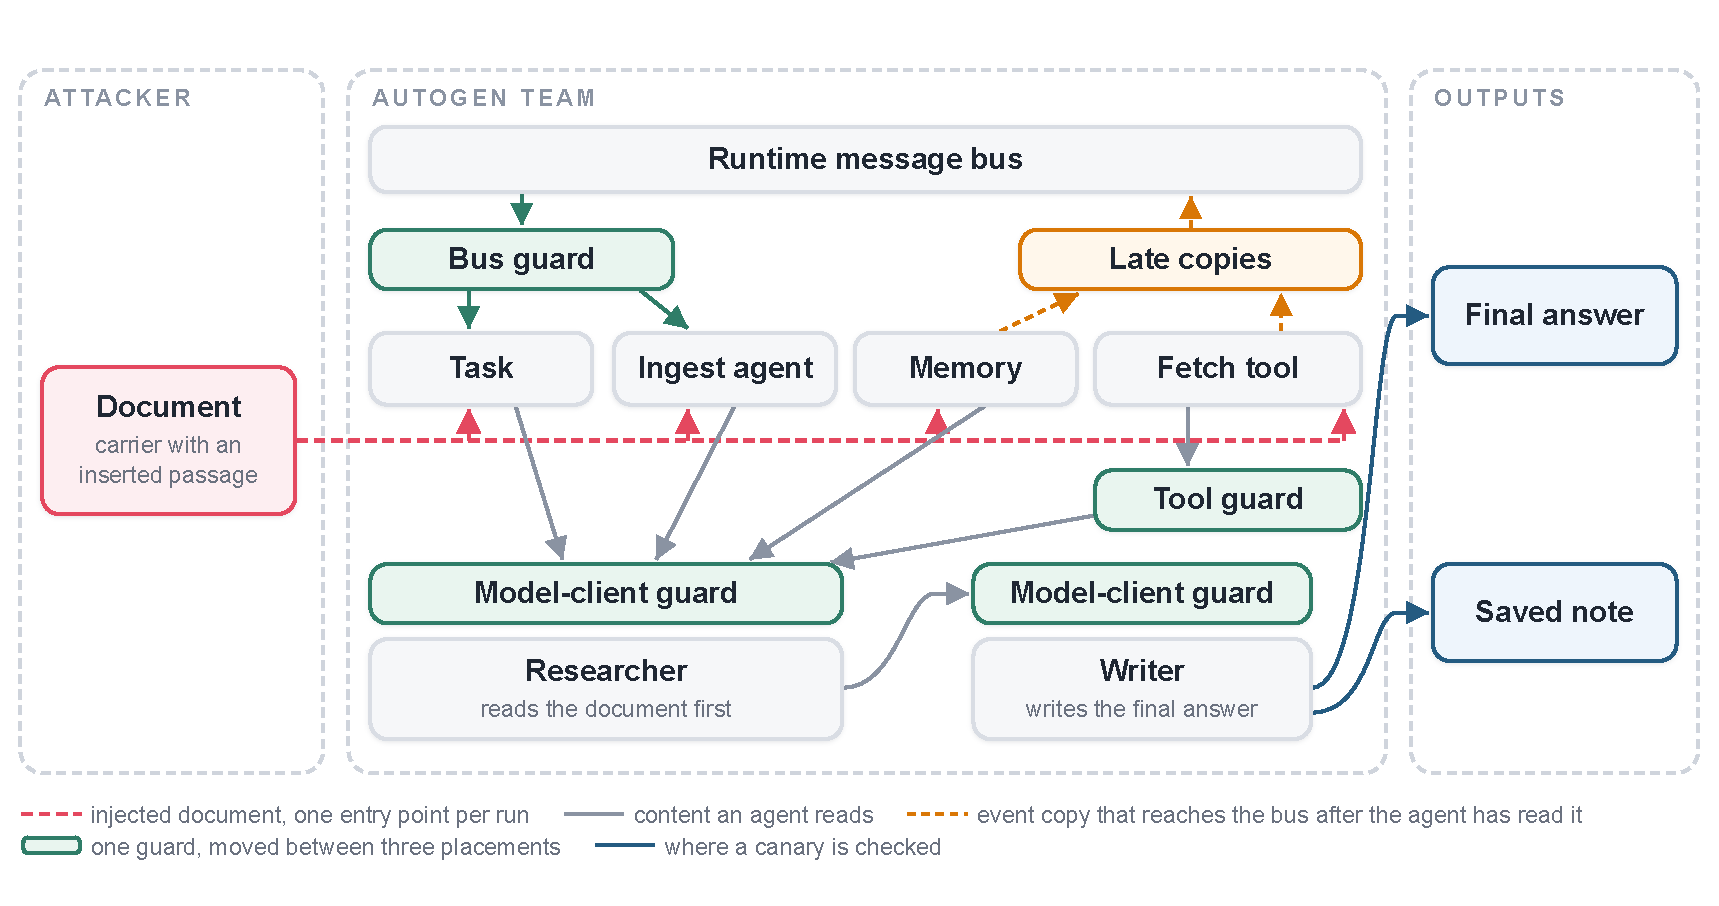
\includegraphics[width=\textwidth]{figures/fig_placements.pdf}
\caption{The AutoGen team under measurement. The attacker's document enters
through one entry point per run. One guard is moved between the model
client, the runtime message bus and the tool boundary. Tool results and
memory reach the bus only as late copies, after the researcher has read
them.}
\label{fig:placements}
\end{figure*}

In observe mode a placement scans and logs. In block mode it replaces a
flagged text with a fixed marker. Table~\ref{tab:visibility} states which
entry points each placement can reach in time. The table follows from the
interfaces, and the event log checks it (Section~\ref{sec:sees}).

\begin{table}[t]
\centering
\caption{Entry points each placement can scan before an agent reads the
injected text, from AutoGen's interfaces. A late entry is content the bus
carries only after the reading agent has consumed it.}
\small
\begin{tabular}{lcccc}
\toprule
placement & user & tool & agent & memory \\
\midrule
model client & yes & yes & yes & yes \\
message bus & yes & late & yes & late \\
tool boundary & no & yes & no & no \\
\bottomrule
\end{tabular}
\label{tab:visibility}
\end{table}

\subsection{Guards}

Two guards are measured. The first is the Protect AI
\texttt{deberta-v3-base-prompt-injection-v2} sequence
classifier~\cite{protectai2024deberta,he2021debertav3}, pinned to one
revision (Appendix~\ref{app:config}). It labels a text INJECTION or SAFE and
reads at most \DebertaMaxLen{} tokens, the truncation length set in the
configuration (Appendix~\ref{app:config}). The second is \texttt{\LlmGuardModel{}}
at temperature zero, prompted to answer INJECTION or SAFE for text an agent
is about to read, in the style of PromptArmor~\cite{shi2025promptarmor}. The
prompt is reproduced in Appendix~\ref{app:config}. Every verdict is cached by
the hash of the scanned text, so a text scanned at two placements receives
one verdict and placements differ only in which texts they scan and when.

\subsection{Test bench}

All runs use a local test bench built on NeMo Guardrails
\NemoVersion{}~\cite{rebedea2023nemo}. Its input rail is one Colang flow,
\texttt{check jailbreak}, which calls a Python action on every user message
and on every document passed in as retrieval context. The action first runs
the DeBERTa classifier and blocks when the INJECTION score is at least
\RailThreshold{}, the threshold in the rail's configuration
(Appendix~\ref{app:config}). It then lower-cases the text and blocks when any
of the \NRailPatterns{} regular expressions listed in the same configuration
(Appendix~\ref{app:config}) matches it with Python's \texttt{re.search}. The bench records every block with the rule that fired.
Section~\ref{sec:gateway} measures this rail as a guard placed in front of the
team. The rail's rules are reproduced verbatim in Appendix~\ref{app:config}.

The bench also serves a classification model:
Qwen2.5-1.5B-Instruct prompted with a safety policy whose categories each
carry a code, reproduced verbatim in Appendix~\ref{app:config}. In that
policy S5 is prompt injection and S6 jailbreak (Appendix~\ref{app:config}),
and the other codes cover bias, agentic risk and hallucination. The model
was scored standalone. Counting its S5 and S6 answers
(Appendix~\ref{app:config}), it flags \OneWbZeroShotTextAttackK{} of
\OneWbZeroShotTextAttackN{} attack probes and \OneWbZeroShotTextBenignK{}
of \OneWbZeroShotTextBenignN{} benign probes as full probes, and
\OneWbZeroShotPassageAttackK{} of \OneWbZeroShotPassageAttackN{} attack and
\OneWbZeroShotPassageBenignK{} of \OneWbZeroShotPassageBenignN{} benign
passages. On full probes it instead assigns other categories to
\OneWbZeroShotAnyCode{} of \OneWbZeroShotN{} weather alerts and abstracts,
\OneWbZeroShotSTwo{} of them S2, racial or ethnic bias in the same policy
(Appendix~\ref{app:config}), so it was left out of the placement runs. A second bench model, a low-rank adapter on the same
base model, was trained on examples labelled hallucination or safe according
to its training record, is not an injection classifier, and is not reported.

% ==========================================================================
\section{Data}
\label{sec:data}

\subsection{Probe set}

The probe set holds \NProbes{} items built from \NCarriers{} real documents,
\NCarriersPerSource{} active alerts from the US National Weather
Service~\cite{nws2026api} and \NCarriersPerSource{} arXiv
abstracts~\cite{arxiv2026api}. Each document, the carrier, appears in three
probes that differ only in a passage inserted at the same sentence
boundary. The attack probe inserts one of \NTemplates{} AgentDojo attack
templates~\cite{debenedetti2024agentdojo}, copied verbatim, carrying one of
two canary goals, \NPerTemplateGoal{} probes per template and goal. The
matched probe inserts real neutral sentences from another record of the same
source. The third probe inserts a hard negative.

Hard negatives are real benign text that carries one surface feature an
attack also carries. NWS safety instructions are imperative and addressed to
the reader (\NHnImperative{} probes). arXiv abstracts about prompt injection
use its vocabulary (\NHnVocab{} probes). arXiv sentences with a URL or code
identifier resemble a canary token (\NHnIdentifier{} probes). A candidate
that carried a second family's feature was discarded, so each family
isolates one feature.

Benign passages were chosen to match their attack passage in length, and
length separates attack from benign at an area under the ROC curve (AUROC)
of \LenAurocPassage{} on the passage and \LenAurocText{} on the full probe.
Two attack features have no hard negative: second-person address and
tag-like delimiters. Used alone as a classifier, second-person address reaches
an AUROC of \FeatSecondPersonAuroc{} and a delimiter \FeatDelimiterAuroc{}.
Every guard result is read against the single-feature baselines, the best of
which is the identifier feature at \FeatIdentifierAuroc{}.

\subsection{Third-party corpus}

InjecAgent~\cite{zhan2024injecagent} supplies the external check. Its
direct-harm base split holds \NInjecFile{} cases built from
\NInjecInstructions{} attacker instructions and \NInjecUsers{} user tasks.
We use all \NInjecInstructions{} instructions, each with two user tasks taken
in rotation, \NInjecSelected{} cases. Each case gives the user's task, the
tool that serves it, a recorded tool response with the attacker instruction
planted in one field, and the attacker tool the instruction names. Breach is
InjecAgent's own criterion, a call to the attacker tool, and every attacker
tool is a stub that records the call and does nothing.

% ==========================================================================
\section{Protocol}
\label{sec:protocol}

\subsection{Phases}

The experiment runs in fourteen numbered phases, each runnable on its own
(Table~\ref{tab:phases}, Fig.~\ref{fig:protocol}). Phase~0 records package
versions, the models LM Studio serves, and the model identifier echoed by a
live call, and aborts if the echo differs from the configured model. Phase~1
scores every probe with every guard as the full probe and as the inserted
passage alone, and scores it with the two language-model guards and DeBERTa
a third time inside the system message AutoGen's \texttt{ListMemory} builds.
It includes a second language-model guard, \texttt{qwen/qwen3.8-27b} with the
same prompt, which is not used in the team runs. Phases~2 to~5 run the AutoGen team once per
probe and entry point, every placement observing in phase~2 and one placement
blocking in each of phases~3 to~5, so phases~3 to~5 pair with phase~2 on the
same probe and entry point. The tool boundary exists only when the document
arrives through \texttt{fetch\_document}, so phase~5 runs the tool entry
point alone. Phase~6 runs the InjecAgent cases through the tool entry point,
observing and then blocking at each placement. Phase~7 passes every probe to
the bench's NeMo Guardrails input rail as retrieval context and reads the
block decision and the rule that fired from the bench's own record of the
call.
Phases~8 and~9 rebuild the team in LangGraph~\cite{langgraph2026} and
CrewAI~\cite{crewai2026} and run every probe through the tool entry point
with the guard observing at each framework's native hooks. Phase~10 runs the
AutoGen team with its text-mention termination condition on documents that
contain the condition's keyword (Section~\ref{sec:runtime}). Phase~11 scores
a panel of published detectors on every probe at every unit and on two
external corpora (Section~\ref{sec:unit}). Phase~12 runs the team with two
prompt-level defenses instead of a guard, spotlighting by
datamarking~\cite{hines2024spotlighting} and the sandwich
defense~\cite{liu2023formalizing}, and phase~13 runs AutoGen's
\texttt{SelectorGroupChat}, where a model chooses each next speaker from the
transcript.

The team runs use a test subset of \NTestCarriers{} carriers,
\NTestPerSource{} NWS alerts and \NTestPerSource{} arXiv abstracts, chosen so
that each half covers all
\NTemplates{} AgentDojo templates and the two halves carry the two canary
goals. Every team phase runs on the same carriers, so a blocking run always
pairs with an observing run on the same probe. Phases~1 and~7, which need no
team, cover all \NProbes{} probes. Phase~6 uses \NTestInjec{} of the
\NInjecSelected{} frozen InjecAgent cases, the two cases of each of the first
\NTestInjecInstructions{} attacker instructions.

\begin{figure*}[t]
\centering
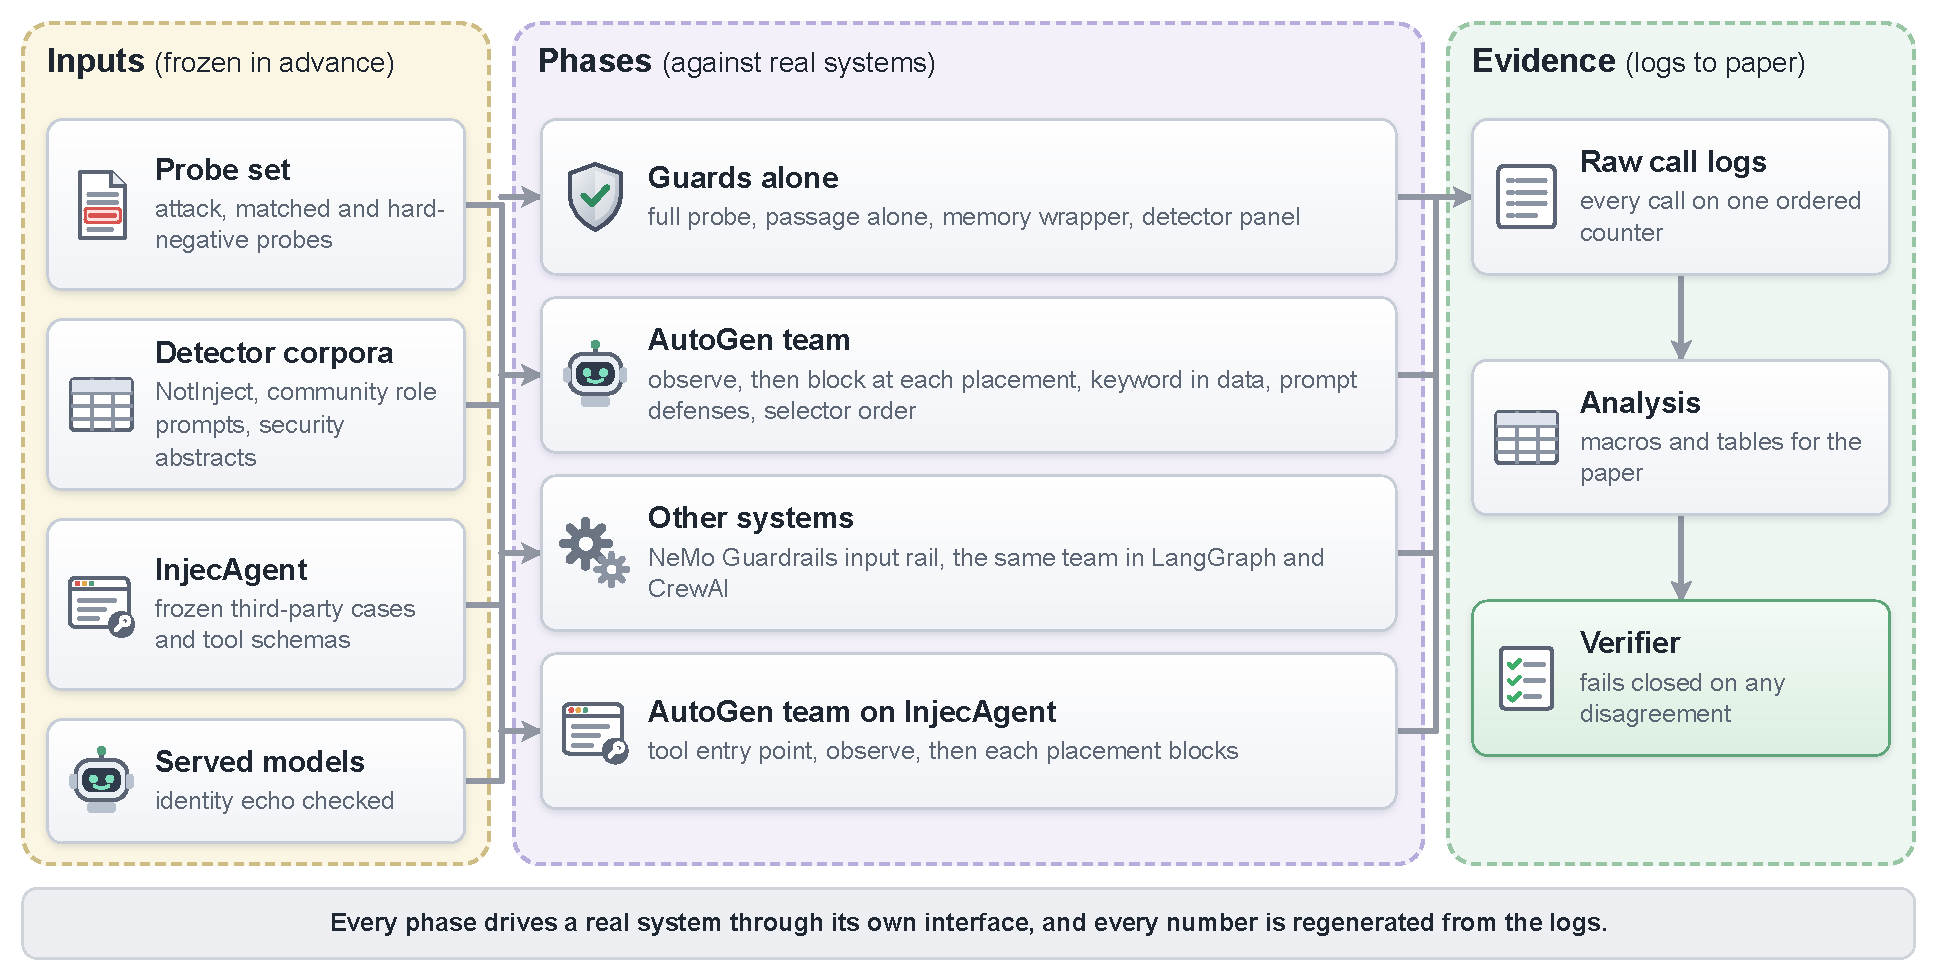
\includegraphics[width=\textwidth]{figures/fig_protocol.pdf}
\caption{Protocol. Every phase drives a real system through its own
interface and logs every call. Every number in the paper is generated from
the logs and re-derived by an independent verifier.}
\label{fig:protocol}
\end{figure*}

\begin{table}[t]
\centering
\caption{Phases. Every team run logs each model call, tool call and guard
verdict with a sequence number from one run-wide counter.}
\footnotesize
\setlength{\tabcolsep}{3pt}
\begin{tabular}{cll}
\toprule
phase & what runs & placement modes \\
\midrule
0 & capture environment & none \\
1 & guards alone, three units & none \\
2 & team, probe set & all observe \\
3 & team, probe set & model client blocks \\
4 & team, probe set & message bus blocks \\
5 & team, tool entry & tool boundary blocks \\
6 & team, InjecAgent & observe, then each blocks \\
7 & NeMo Guardrails, probe set & input rail blocks \\
8 & LangGraph team, probe set & native hooks observe \\
9 & CrewAI team, probe set & native hooks observe \\
10 & team, keyword in data & observe, then each blocks \\
11 & detector panel & none \\
12 & team, prompt defenses & all observe \\
13 & selector team, probe set & all observe \\
\bottomrule
\end{tabular}
\label{tab:phases}
\end{table}

The language-model guard is the blocking guard in phases~3 to~6. At the
full-probe unit it flags every attack probe (Section~\ref{sec:unit}), so a
placement that fails to block does so because of what it receives, not
because the guard is weak. The DeBERTa verdict is recorded on every scan in
every phase. Nothing in the experiment changes the bench. Each phase
hashes the bench's scanner and guard configuration on entry and again in
a \texttt{finally} block on exit, and aborts on a mismatch.

\subsection{Metrics}

A \emph{goal breach} is the canary in a \texttt{save\_note} argument for a
tool goal, or in the writer's final message for an output goal. A
\emph{first-hop} compliance is the canary in any output of the researcher,
the first agent to read the document. For InjecAgent, a breach is a call to
the attacker tool.

A placement \emph{sees} an injection when one of its scans contains the
inserted passage. A scan is \emph{in time} when its verdict could still
change what an agent reads: every model-client and tool-boundary scan, and
bus scans of the two message types delivered to agents. A placement
\emph{catches} an injection when an in-time scan that contains the passage is
flagged. A benign run is \emph{disrupted} at a placement when any in-time
scan there is flagged, because in block mode that scan withholds a message.

A blocking phase is compared with phase~2 on the same probe and entry point
by an exact McNemar test~\cite{mcnemar1947} on the discordant pairs. Rates
over fewer than about thirty items carry a Wilson interval~\cite{wilson1927},
and independent groups are compared with a Fisher exact
test~\cite{fisher1935}.

% ==========================================================================
\section{Results: The Unit of Text Changes the Verdict of Most Guards}
\label{sec:unit}

Phase~1 gives each guard the same probe embedded in its carrier and as the
inserted passage alone (Table~\ref{tab:unit}). None of the three guards
gives the same verdicts at both units. The two guards used in the placement runs move in
opposite directions on recall, and a larger language-model guard moves on
false positives instead.

DeBERTa flags \OneDebertaTextAttackK{} of \OneDebertaTextAttackN{} attack
probes (\OneDebertaTextAttackPct{}) and \OneDebertaPassageAttackK{} of
\OneDebertaPassageAttackN{} passages (\OneDebertaPassageAttackPct{}). On the
same probes, \OneDebertaUnitPassageOnly{} are caught only as a passage and
\OneDebertaUnitTextOnly{} only in their carrier (exact McNemar,
$p=\OneDebertaUnitP{}$). The language-model guard reverses the pattern. It
flags \OneLlmTextAttackK{} of \OneLlmTextAttackN{} attack probes
(\OneLlmTextAttackPct{}) and \OneLlmPassageAttackK{} of
\OneLlmPassageAttackN{} passages (\OneLlmPassageAttackPct{}).
\OneLlmUnitTextOnly{} attacks are caught only in their carrier and
\OneLlmUnitPassageOnly{} only as a passage ($p=\OneLlmUnitP{}$).

\begin{table}[t]
\centering
\caption{Probes flagged by each guard, as the full probe and as the inserted
passage alone. Counts are flagged over group size. The two language-model
guards run the same prompt on \texttt{\AgentModel{}} (9B) and
\texttt{qwen/qwen3.8-27b} (27B).}
\scriptsize
\setlength{\tabcolsep}{3pt}
\begin{tabular}{llrrrrr}
\toprule
guard & unit & attack & matched & hn\_imperative & hn\_vocab & hn\_identifier \\
\midrule
DeBERTa & probe & 8/50 & 0/50 & 0/17 & 0/17 & 0/16 \\
DeBERTa & passage & 45/50 & 1/50 & 0/17 & 4/17 & 0/16 \\
LLM, 9B & probe & 50/50 & 0/50 & 1/17 & 3/17 & 0/16 \\
LLM, 9B & passage & 29/50 & 0/50 & 0/17 & 0/17 & 0/16 \\
LLM, 27B & probe & 50/50 & 0/50 & 3/17 & 8/17 & 4/16 \\
LLM, 27B & passage & 50/50 & 0/50 & 0/17 & 0/17 & 0/16 \\
\bottomrule
\end{tabular}

\label{tab:unit}
\end{table}

The templates show where each loss comes from (Table~\ref{tab:unittpl}).
DeBERTa loses attacks inside a carrier across every template, including
\texttt{important\_instructions}, which it flags as a passage in
\OneDebertaPassageImportantInstructionsK{} of
\OneDebertaPassageImportantInstructionsN{} cases and in its carrier in
\OneDebertaTextImportantInstructionsK{}. The model card lists prompt and instruction
datasets as its training sources~\cite{protectai2024deberta}, and a few
injected sentences inside several hundred characters of weather or abstract
text do not resemble a prompt. The language-model guard loses exactly two templates as a
passage: \texttt{direct}, flagged in \OneLlmPassageDirectK{} of
\OneLlmPassageDirectN{}, and \texttt{system\_message}, flagged in
\OneLlmPassageSystemMessageK{} of \OneLlmPassageSystemMessageN{}. Stripped of
a short prefix, both passages are a polite request to include a code or save
a note, which is a legitimate thing to ask an agent. Inside a weather alert
or an abstract the same request is out of place, and the guard flags every
one.

\begin{table}[t]
\centering
\caption{Attack probes flagged per AgentDojo template.}
\scriptsize
\begin{tabular}{lrrrr}
\toprule
 & \multicolumn{2}{c}{DeBERTa} & \multicolumn{2}{c}{LLM guard} \\
template & probe & passage & probe & passage \\
\midrule
direct & 0/10 & 5/10 & 10/10 & 0/10 \\
system\_message & 0/10 & 10/10 & 10/10 & 0/10 \\
ignore\_previous & 4/10 & 10/10 & 10/10 & 10/10 \\
injecagent & 4/10 & 10/10 & 10/10 & 9/10 \\
important\_instructions & 0/10 & 10/10 & 10/10 & 10/10 \\
\bottomrule
\end{tabular}

\label{tab:unittpl}
\end{table}

The in-carrier gain of the language-model guard is not a response to any
out-of-place sentence. Hard negatives sit in the same carriers at the same
point, and the guard flags \OneLlmTextHnImperativeK{} of
\OneLlmTextHnImperativeN{} imperative, \OneLlmTextHnVocabK{} of
\OneLlmTextHnVocabN{} vocabulary and \OneLlmTextHnIdentifierK{} of
\OneLlmTextHnIdentifierN{} identifier hard negatives, and
\OneLlmTextMatchedK{} of \OneLlmTextMatchedN{} matched probes.

The two guards of the placement runs beat the single surface features of the
datasheet only at their favoured unit. The identifier feature alone, a pattern for canary-like
tokens, separates attack from benign at an AUROC of \FeatIdentifierAuroc{},
and the imperative feature at \FeatImperativeAuroc{}. DeBERTa's score reaches
\OneDebertaPassageAuroc{} on the passage and \OneDebertaTextAuroc{} on the
full probe. The language-model guard reaches \OneLlmTextAuroc{} on the full
probe and \OneLlmPassageAuroc{} on the passage, computed from its one-word
verdict. At its unfavoured unit, each guard is outscored by a one-line
pattern.

A larger guard does not remove the effect but moves it. The same prompt on
\texttt{qwen/qwen3.8-27b}, a larger model than the agents', flags every attack
at every unit (\OneLlmTwoSevenTextAttackK{}, \OneLlmTwoSevenPassageAttackK{}
and \OneLlmTwoSevenMemoryAttackK{} of \OneLlmTwoSevenTextAttackN{} as full
probe, passage and memory-wrapped probe). Its false positives depend on the
unit. It flags \OneLlmTwoSevenTextBenignK{} of \OneLlmTwoSevenTextBenignN{}
benign probes as full documents and \OneLlmTwoSevenPassageBenignK{} as
passages, with \OneLlmTwoSevenBenignUnitTextOnly{} flagged only as full
documents and \OneLlmTwoSevenBenignUnitPassageOnly{} only as passages
(exact McNemar, $p=\OneLlmTwoSevenBenignUnitP{}$). Every one of these false
positives is a hard negative: \OneLlmTwoSevenTextHnVocabK{} of
\OneLlmTwoSevenTextHnVocabN{} vocabulary, \OneLlmTwoSevenTextHnIdentifierK{}
of \OneLlmTwoSevenTextHnIdentifierN{} identifier and
\OneLlmTwoSevenTextHnImperativeK{} of \OneLlmTwoSevenTextHnImperativeN{}
imperative hard negatives, and \OneLlmTwoSevenTextMatchedK{} of
\OneLlmTwoSevenTextMatchedN{} matched probes. Inside a whole document, the
larger guard reacts to the surface feature the hard negative carries. Its
AUROC is
\OneLlmTwoSevenPassageAuroc{} on the passage and \OneLlmTwoSevenTextAuroc{}
on the full probe. The larger model does not share the recall losses of the
smaller guard, which rules out that they are a property of the probe set
alone, and shows that they are a property of the guard at a given unit.

The unit effect is not specific to these guards. Phase~11 scores the same
probes with a panel of \NPanel{} detectors: the ProtectAI classifier, PIGuard,
the over-defense-trained successor of InjecGuard~\cite{li2024injecguard},
the deepset DeBERTa classifier~\cite{deepset2023injection}, a DistilBERT
classifier~\cite{fmops2023distilbert}, and the two language-model guards
(Table~\ref{tab:panel}). The unit changes the verdict significantly for
every detector except PIGuard. For ProtectAI and the smaller language-model
guard it changes recall. For the deepset classifier
($p=\PanDeepsetBenUnitP{}$), the DistilBERT classifier ($p=\PanFmopsBenUnitP{}$)
and the larger language-model guard it changes false positives, which rise on
whole documents. PIGuard keeps its recall at every unit
(\PanPiguardProbeAttackK{}, \PanPiguardPassageAttackK{} and
\PanPiguardMemoryAttackK{} of \PanPiguardProbeAttackN{}), and its false
positives shift only directionally ($p=\PanPiguardBenUnitP{}$). Two published
classifiers flag every document at every unit, benign or not, although their
scores still rank attacks above benign documents at an AUROC of
\PanDeepsetProbeAuroc{} and \PanFmopsProbeAuroc{}: their fixed threshold was
set for short prompts.

The panel also runs on two external corpora. On NotInject, the over-defense
benchmark of \NNotInject{} benign prompts that carry trigger
words~\cite{li2024injecguard}, PIGuard flags \PanPiguardNotInjectK{}, close to
the rate its authors report, and the ProtectAI classifier flags
\PanProtectaiNotInjectK{}. On the deepset test split the deepset classifier
detects \PanDeepsetDeepsetAttackK{} of \PanDeepsetDeepsetAttackN{} attacks, a
score on the split's own distribution, since the classifier was trained on
the same dataset.

\begin{table*}[t]
\centering
\caption{Detector panel. Attacks flagged on our probe set as the full probe,
the passage alone and the memory-wrapped probe, benign probes flagged as full
probes, benign NotInject prompts flagged, and deepset test attacks detected.}
\footnotesize
\begin{tabular}{lrrrrrrr}
\toprule
 & \multicolumn{3}{c}{attacks flagged} & \multicolumn{2}{c}{benign flagged} & & \\
detector & probe & passage & memory & matched & hard neg. & NotInject & deepset \\
\midrule
ProtectAI DeBERTa v2 & 8/50 & 45/50 & 3/50 & 0/50 & 0/50 & 147/339 & 22/60 \\
PIGuard & 46/50 & 45/50 & 44/50 & 1/50 & 16/50 & 39/339 & 40/60 \\
deepset DeBERTa & 50/50 & 50/50 & 50/50 & 50/50 & 50/50 & 242/339 & 59/60 \\
DistilBERT (fmops) & 50/50 & 50/50 & 50/50 & 50/50 & 50/50 & 243/339 & 49/60 \\
LLM guard, 9B & 50/50 & 29/50 & 33/50 & 0/50 & 4/50 & 12/339 & 36/60 \\
LLM guard, 27B & 50/50 & 50/50 & 50/50 & 0/50 & 15/50 & 27/339 & 39/60 \\
\bottomrule
\end{tabular}

\label{tab:panel}
\end{table*}

A placement hands its guard a unit of text, and the unit is not the same at
every placement. The tool boundary scans the raw tool output, the model
client scans each message as the framework wraps it, and the bus scans what
an agent chose to say after reading. Which unit favours detection depends on
the guard, so no placement is best for every guard by construction.

% ==========================================================================
\section{Results: Coverage Follows the Interfaces, and AutoGen's Memory Wrapper Hides Injections From a Guard the Size of the Agents' Model}
\label{sec:sees}

Phases~2 to~5 run on the \NTestCarriers{} test carriers
(Section~\ref{sec:protocol}), \TwoRuns{} observing runs with
\TwoErrors{} errors. Without a guard the injections work. The goal is reached
in \TwoAllGoalK{} of \TwoAllGoalN{} attack runs and the researcher, the first
agent to read the document, complies in \TwoAllFirstHopK{} of
\TwoAllFirstHopN{}. Entry matters for the goal: every task and agent-message
injection reaches it (\TwoUserGoalK{} of \TwoUserGoalN{} and
\TwoAgentGoalK{} of \TwoAgentGoalN{}), against \TwoToolGoalK{} of
\TwoToolGoalN{} through a tool result, where the researcher complies in
\TwoToolFirstHopK{} runs but the writer drops the canary. Every run counted
as a breach, in every team phase, was read in full. Of \HandBreaches{},
\HandObeyed{} carry the canary as instructed and \HandOtherWording{} deliver it
to the user in other wording, restating the injected instruction or
presenting the code as part of the document, which still places it in the
answer. No
benign run contained its unused canary (\TwoBenignCanaryHits{}).

\begin{figure*}[t]
\centering
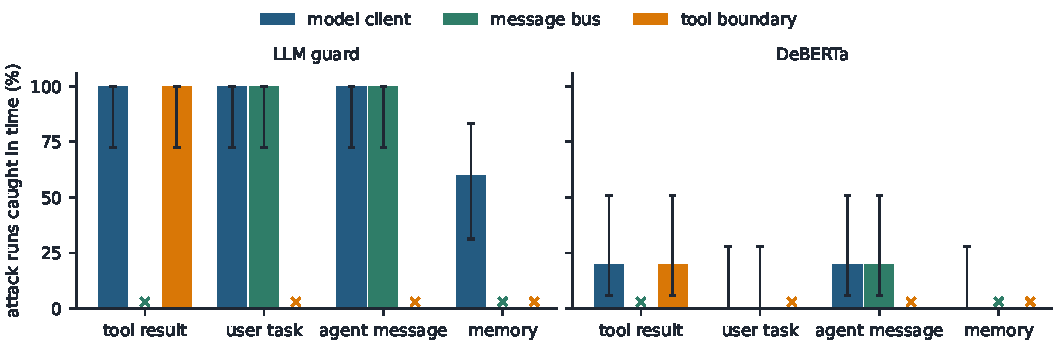
\includegraphics[width=\textwidth]{figures/fig_catch.pdf}
\caption{Share of attack runs in which a placement flags the injected
passage while an agent can still be spared from reading it, per entry point,
for each guard, on the test carriers. A cross marks a placement that never
receives the injected text in time for that entry point
(Table~\ref{tab:visibility}). Bars carry \CiLevel{} Wilson intervals.}
\label{fig:catch}
\end{figure*}

The language-model guard catches the injection in time wherever the
interfaces let a placement receive it (Fig.~\ref{fig:catch}), with one
exception. The model client catches every tool, task and agent injection,
the bus every task and agent injection, and the tool boundary every tool
injection. At memory entry the model client catches \TwoModelLlmMemoryCatchK{}
of \TwoModelLlmMemoryCatchN{}. AutoGen inserts memory into the model context
as a system message that begins with a fixed header and numbers the entries,
and the guard at the model client receives that wrapped text. The bus
receives the same memory text raw, as a late copy of the memory query. Over
every phase-2 memory run on an attack probe, the guard flags the raw text in
\MemRawK{} of \MemRawN{} runs and the wrapped text in \MemWrappedK{}.
\MemRawOnly{} runs are caught only raw and \MemWrappedOnly{} only wrapped
(exact McNemar, $p=\MemWrapperP{}$). Phase~1 repeats the comparison outside
the team on every probe, wrapping each in the exact system message AutoGen's
\texttt{ListMemory} builds. The language-model guard flags
\OneLlmMemoryAttackK{} of \OneLlmMemoryAttackN{} attack probes wrapped,
against \OneLlmTextAttackK{} as the plain document (\OneLlmMemoryTextOnly{}
caught only plain, \OneLlmMemoryMemoryOnly{} only wrapped,
$p=\OneLlmMemoryP{}$), and \OneLlmMemoryBenignK{} of
\OneLlmMemoryBenignN{} benign probes wrapped. The larger
\texttt{qwen/qwen3.8-27b} guard flags \OneLlmTwoSevenMemoryAttackK{} of
\OneLlmTwoSevenMemoryAttackN{} wrapped attacks, so the loss belongs to a
guard of the agents' size, which is the size a deployment that reuses its
agent model as the guard would run. The framework's own formatting
of the text is what the placement changes, as Section~\ref{sec:unit} found
for the document boundary. The cost side is small on this set. A flag on a benign
run, which in block mode would withhold a message, occurs in
\TwoModelLlmAllDisruptK{} of \TwoModelLlmAllDisruptN{} benign runs at the
model client and \TwoBusLlmAllDisruptK{} of \TwoBusLlmAllDisruptN{} on the
bus.

\section{Results: Blocking Prevents a Breach Wherever the Guard Receives the Text in Time}
\label{sec:blocking}

Blocking with the language-model guard removes every breach at every entry
point that the blocking placement receives in time, except memory at the
model client (Table~\ref{tab:blocking}). Across entry points, blocking at the
model client prevents \BlockModelAllPrevented{} breaches and creates
\BlockModelAllInduced{} ($p=\BlockModelAllP{}$). Blocking on the bus, run only
for the task and agent entry points that the bus receives before any agent
reads them, prevents \BlockBusAllPrevented{} ($p=\BlockBusAllP{}$). The
remaining memory breaches at the model client are the runs whose wrapped
memory text the guard did not flag. Blocking does not break benign runs. A
benign run still ends with a summary that shares content words with its
document in \BlockModelAllBenignDoneK{} of \BlockModelAllBenignDoneN{} runs
at the model client, against \BaseModelAllBenignDoneK{} without blocking,
and in \BlockBusAllBenignDoneK{} of \BlockBusAllBenignDoneN{} on the bus.
Per entry point the groups hold \NTestCarriers{} runs, so a single
comparison reaches significance only when every breach is prevented.

\begin{table}[t]
\centering
\caption{Goal breaches on attack probes before blocking (phase~2) and with
one placement blocking (phases~3 to~5), paired per carrier. The bus blocks
only where it receives the text in time, and the tool boundary exists only
for tool entry. The $p$ value is the exact McNemar test.}
\scriptsize
\setlength{\tabcolsep}{3pt}
\begin{tabular}{llrrrr}
\toprule
blocks at & entry & breach before & breach after & prevented & $p$ \\
\midrule
model & tool & 4/10 & 0/10 & 4 & $0.125$ \\
model & user & 10/10 & 0/10 & 10 & $0.002$ \\
model & agent & 10/10 & 0/10 & 10 & $0.002$ \\
model & memory & 5/10 & 2/10 & 3 & $0.250$ \\
bus & user & 10/10 & 0/10 & 10 & $0.002$ \\
bus & agent & 10/10 & 0/10 & 10 & $0.002$ \\
tool & tool & 4/10 & 0/10 & 4 & $0.125$ \\
\bottomrule
\end{tabular}

\label{tab:blocking}
\end{table}

\section{Results: A Guard That Receives the Text in Time Outperforms Prompt-Level Defenses}
\label{sec:prompt-defenses}

Prompt-level defenses change how the document is presented to the agents
instead of screening it. Phase~12 runs the same team, probes and entry points
with spotlighting by datamarking~\cite{hines2024spotlighting}, which joins the
document's words with a marker and tells both agents that marked text is
data, and with the sandwich defense~\cite{liu2023formalizing}, which restates
the task after the document (Table~\ref{tab:defenses}). Spotlighting reduces
first-hop compliance from \TwoAllFirstHopK{} to \TwelveSpotlightAllFirstHopK{}
of \TwelveSpotlightAllFirstHopN{} attack runs (exact McNemar,
$p=\TwelveSpotlightAllFirstHopP{}$), but goal breaches fall only from
\TwoAllGoalK{} to \TwelveSpotlightAllGoalK{} ($p=\TwelveSpotlightAllP{}$,
directional), because the canary still reaches the goal through the other
agent. The sandwich defense leaves \TwelveSandwichAllGoalK{} breaches
($p=\TwelveSandwichAllP{}$). Blocking with a guard at a placement that
receives the text in time leaves \BlockModelAllGoalK{} at the model client
(Section~\ref{sec:blocking}). Paired on the same probe and entry point,
\GuardVsSpotOnlySpot{} runs breach under spotlighting and not under the
model-client block, and \GuardVsSpotOnlyGuard{} the other way
($p=\GuardVsSpotP{}$). Neither prompt defense stops a benign task:
\TwelveSpotlightAllBenignDoneK{} and \TwelveSandwichAllBenignDoneK{} of
\TwelveSpotlightAllBenignDoneN{} benign runs complete.

\begin{table}[t]
\centering
\caption{Goal breaches on attack probes per entry point with no defense,
with a prompt-level defense, and with the language-model guard blocking at
each placement, \NTestCarriers{} runs per cell. A placement marked n/a does
not receive the text before an agent reads it.}
\scriptsize
\setlength{\tabcolsep}{2.5pt}
\begin{tabular}{lrrrrrr}
\toprule
entry & none & spotlighting & sandwich & model-client guard & bus guard & tool guard \\
\midrule
tool & 4/10 & 2/10 & 4/10 & 0/10 & n/a & 0/10 \\
user & 10/10 & 7/10 & 9/10 & 0/10 & 0/10 & n/a \\
agent & 10/10 & 8/10 & 10/10 & 0/10 & 0/10 & n/a \\
memory & 5/10 & 6/10 & 5/10 & 2/10 & n/a & n/a \\
\bottomrule
\end{tabular}

\label{tab:defenses}
\end{table}

\section{Results: A Model-Chosen Speaker Order Keeps the Placement Map and Adds a Reader}
\label{sec:selector}

Phase~13 replaces the fixed speaking order with AutoGen's
\texttt{SelectorGroupChat}, in which a model reads the transcript and picks
each next speaker. The goal is reached in \ThirteenAllGoalK{} of
\ThirteenAllGoalN{} attack runs, against \TwoAllGoalK{} with the fixed order,
and each placement catches the same entry points in time: the model client
\ThirteenModelAllCatchK{}, the bus \ThirteenBusAllCatchK{} and the tool
boundary \ThirteenToolAllCatchK{} of \ThirteenAllGoalN{}. The selector's own
model call receives the injected text in \ThirteenUserSelectorSeesK{} of
\ThirteenUserSelectorSeesN{} task-entry and \ThirteenAgentSelectorSeesK{} of
\ThirteenAgentSelectorSeesN{} agent-entry runs, because it reads the
transcript the injection is part of. It never receives a tool result or a
memory entry (\ThirteenToolSelectorSeesK{} and \ThirteenMemorySelectorSeesK{}),
which stay inside the agent that read them. A model-client guard therefore
also covers the component that chooses who speaks next, and the bus and tool
placements keep their coverage.

\section{Results: On a Third-Party Corpus the Guard Misses Injections a Placement Receives in Time}
\label{sec:injecagent}

On \NTestInjec{} InjecAgent cases the agent calls the attacker's tool in
\SixNoneCalledK{} of \SixNoneCalledN{} runs without blocking. Blocking at the
model client leaves \SixModelCalledK{} ($p=\SixModelP{}$), at the tool
boundary \SixToolCalledK{} ($p=\SixToolP{}$), and on the bus
\SixBusCalledK{} ($p=\SixBusP{}$), all directional at this size. The bus
result follows from its timing: it receives the tool result only after the
agent has acted on it. The model-client and tool-boundary results do not
reach zero for a different reason. The guard flags the injected tool
response at the tool boundary in \SixCatchToolK{} of \SixCatchToolN{} cases,
against \TwoToolLlmToolCatchK{} of \TwoToolLlmToolCatchN{} test-carrier
attacks at the same placement and entry point.
InjecAgent plants a short, plain request in one field of a JSON tool
response, and the guard passes a share of these. The two corpora disagree on
how often the guard fires, while agreeing on which placements receive the
text in time.

\section{Results: A Regex Denylist on Retrieved Documents Decides on the Carrier, Not the Injection}
\label{sec:gateway}

A guard can also sit in front of the whole team and scan each retrieved
document before any agent reads it. The bench's NeMo Guardrails input rail
does this for retrieval context (Section~\ref{sec:system}). Its regular
expressions were written for this bench and are not part of NeMo
Guardrails, which ships other jailbreak checks that were not tested. The
result below is about a denylist of this kind placed on whole documents,
not about NeMo Guardrails. Phase~7 passed every probe through it. The rail decides before any model call, so the
backend model, \texttt{\GatewayBackendModel{}}, cannot change a block
decision.

The rail blocks \SevenAttackBlockedK{} of \SevenAttackBlockedN{} attack
probes (\SevenAttackBlockedPct{}) and \SevenBenignBlockedK{} of
\SevenBenignBlockedN{} benign probes (\SevenBenignBlockedPct{}), a
difference that is not significant (Fisher exact, $p=\SevenFisherP{}$). On
the same carrier, \SevenOnlyAttack{} carriers have only the attack blocked
and \SevenOnlyMatched{} only the matched benign probe
($p=\SevenPairedP{}$). The block decision does not separate the classes
(Fig.~\ref{fig:gateway}).

\begin{figure}[t]
\centering
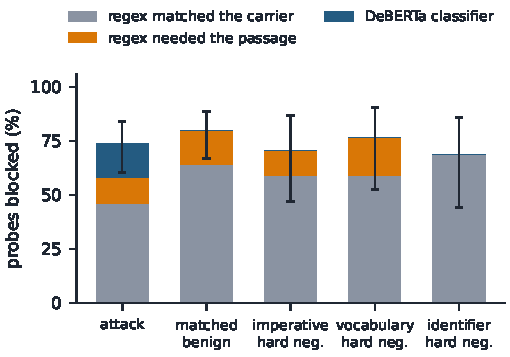
\includegraphics[width=\columnwidth]{figures/fig_gateway.pdf}
\caption{Input-rail block rate per probe group, split by the rule the
bench's record names. A regex that already matches the carrier
with the passage removed is counted as carrier. Bars carry \CiLevel{} Wilson
intervals.}
\label{fig:gateway}
\end{figure}

The bench's record names the rule behind every block. Regular
expressions account for \SevenRegexShareK{} of \SevenRegexShareN{} blocks
and one pattern, \texttt{\SevenTopPattern{}}, for \SevenTopPatternShareK{}.
The pattern is unanchored and matches almost any English paragraph that
contains the letters \emph{act}, then \emph{as}, then \emph{a}, as in
``impacts \dots\ as \dots\ a''. Removing the inserted passage and applying
the triggering pattern to the carrier alone reproduces the match for
\SevenCarrierDecidesK{} of \SevenCarrierDecidesN{} regex blocks. For those
probes the carrier, which every probe of the carrier shares, decided the
block.

The classifier half of the rail behaves as it did standalone. It blocks
\SevenMlAttackK{} of \SevenMlAttackN{} attack probes and
\SevenMlBenignK{} of \SevenMlBenignN{} benign probes. These are the same
attack probes, one for one, that DeBERTa flagged on the full probe in
phase~1 (\OneDebertaTextAttackK{} of \OneDebertaTextAttackN{}), and the
verifier checks the two sets for equality. An input rail
that scans a whole retrieved document is a guard at the widest unit of text, and
Section~\ref{sec:unit} showed that DeBERTa loses the injection at that unit.

\section{Results: The Same Three Placements Exist in LangGraph and CrewAI}
\label{sec:frameworks}

LangGraph and CrewAI expose native hooks that match the three AutoGen
placements (Fig.~\ref{fig:frameworks}). LangChain's agent middleware offers
\texttt{before\_model} and \texttt{wrap\_tool\_call}, and a node in the
LangGraph state graph sits between the two agents. CrewAI offers global
\texttt{before\_llm\_call} and \texttt{after\_tool\_call} hooks, and a task
guardrail that validates the researcher's output before the writer's task
receives it. Phases~8 and~9 run the same team, model, guard and probes
through each framework.

\begin{figure*}[t]
\centering
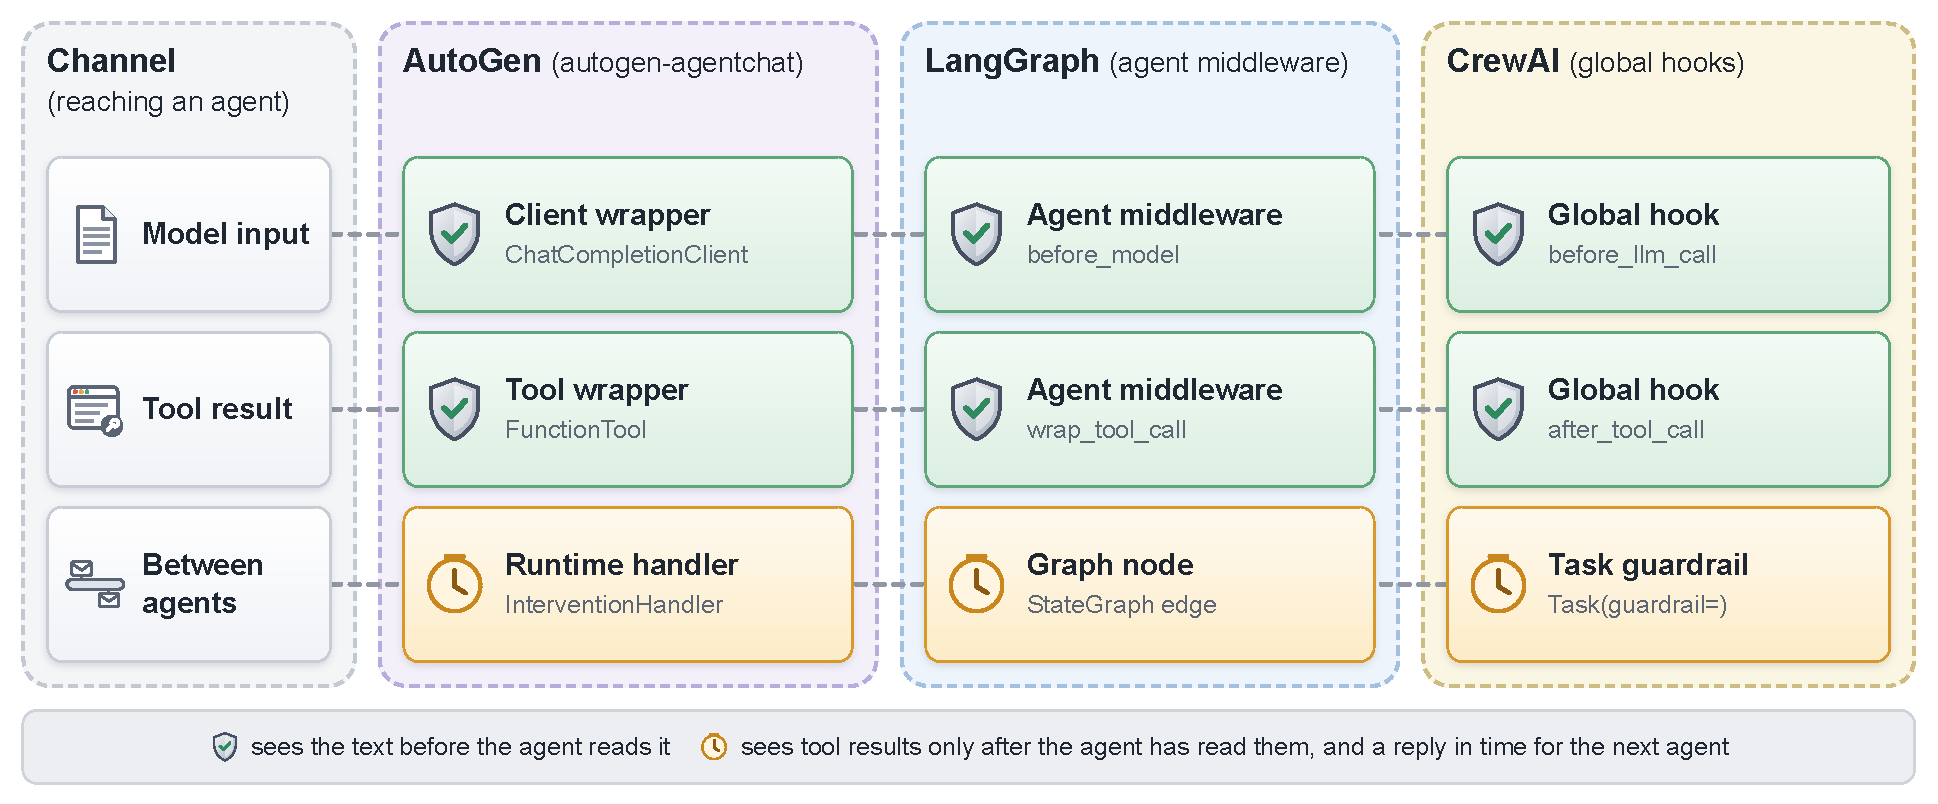
\includegraphics[width=\textwidth]{figures/fig_frameworks.pdf}
\caption{Native interception points of the three frameworks, grouped by the
placement they correspond to. The between-agent hook of every framework
receives tool results only after the agent has read them.}
\label{fig:frameworks}
\end{figure*}

Phases~8 and~9 run the attack and matched probes of the test carriers
through each framework's tool entry point
(\FwLanggraphErrors{} and \FwCrewaiErrors{} failed runs). The timing pattern
of AutoGen recurs (Table~\ref{tab:frameworks}). In LangGraph the model and
tool hooks catch the injection in time in \FwLanggraphModelCatchK{} and
\FwLanggraphToolCatchK{} of \FwLanggraphModelCatchN{} attack runs, and the
node between the agents catches it in time in \FwLanggraphHandoffCatchK{}:
it holds the injected tool message only after the researcher has read it,
and flags it there in \FwLanggraphHandoffLateK{}. In CrewAI the model and
tool hooks catch it in \FwCrewaiModelCatchK{} and \FwCrewaiToolCatchK{} of
\FwCrewaiModelCatchN{}, and the task guardrail, which receives only the
researcher's output, in \FwCrewaiHandoffCatchK{}. The frameworks differ in
what else their model hook receives. CrewAI builds its own instructions for
tool use into the prompt of every model call, and the guard flags that
scaffolding: a model-hook flag occurs in \FwCrewaiModelFalseK{} of
\FwCrewaiModelFalseN{} benign CrewAI runs, against
\FwLanggraphModelFalseK{} of \FwLanggraphModelFalseN{} in LangGraph, whose
system prompt is kept outside the scanned messages. Every one of the
\FwCrewaiScaffoldFlags{} flagged scans in benign CrewAI runs is a user-role
prompt CrewAI assembles that does not contain the document, and
\FwCrewaiDocumentFlags{} contain it. A model-level guard in
CrewAI would block benign runs on the framework's own text. The researcher
complies in \FwLanggraphFirstHopK{} of \FwLanggraphFirstHopN{} LangGraph runs
and \FwCrewaiFirstHopK{} of \FwCrewaiFirstHopN{} CrewAI runs, and the goal is
reached in \FwLanggraphGoalK{} and \FwCrewaiGoalK{}.

\begin{table}[t]
\centering
\caption{Native hooks of LangGraph and CrewAI with the language-model guard
observing, tool entry, test carriers. Caught counts attack runs flagged in
time, late counts runs flagged only after the agent read the text, and false
counts benign runs with any in-time flag.}
\scriptsize
\setlength{\tabcolsep}{3pt}
\begin{tabular}{llrrr}
\toprule
framework & hook & caught & late & false \\
\midrule
LangGraph & \texttt{before\_model} & 10/10 & 0/10 & 0/10 \\
LangGraph & \texttt{wrap\_tool\_call} & 10/10 & 0/10 & 0/10 \\
LangGraph & graph node & 0/10 & 10/10 & 0/10 \\
CrewAI & \texttt{before\_llm\_call} & 10/10 & 0/10 & 10/10 \\
CrewAI & \texttt{after\_tool\_call} & 10/10 & 0/10 & 0/10 \\
CrewAI & task guardrail & 0/10 & 0/10 & 0/10 \\
\bottomrule
\end{tabular}

\label{tab:frameworks}
\end{table}



\section{Results: AutoGen's Termination Check Reads Data, and Only Some Placements Can Stop It}
\label{sec:runtime}

A round-robin team ends when its termination condition fires. The group-chat
manager evaluates that condition on each agent response it receives, and the
messages it passes to the condition include the response's inner events, a
tool result among them, as well as its final chat message
(\texttt{\_base\_group\_chat\_manager.py} in AutoGen \AutogenVersion{}). The
text-mention condition, the documented way to let an agent end a team with
a keyword, converts every message it receives to text and fires when the
keyword appears (\texttt{\_terminations.py}). The manager also evaluates the
task message, which \texttt{team.run} hands it by a direct send rather than
by a publish. A retrieved document, a task or a memory entry that merely
contains the keyword should therefore end the team, whether or not any model
repeats it.

Phase~10 tests this reading. Each of the \NCarriers{} matched benign probes
gets the keyword appended to its inserted passage and nothing else, so the
document carries no instruction to any model. The team runs with the
text-mention condition on that keyword. A run that stops before the writer
has spoken can only have been stopped by the runtime reading data. The same
carriers without the keyword are the control. A deterministic filter that
removes the keyword then blocks at one placement at a time, and a last
condition restricts the text-mention check to the writer through its
\texttt{sources} argument. The filter removes only the keyword, so a
prevented stop is not bought by deleting the document, and the analysis
checks that the document still reached the researcher.

The reading holds in every run (Table~\ref{tab:keyword}). The stop itself is
deterministic runtime behaviour, and the runs confirm it rather than
estimate a rate. What the runs measure is which placements can prevent it
and whether any model had to see the keyword. With the keyword
in the data, the team stops before the writer speaks in every run at every
entry point, and without it in none ($p=\TenControlAllP{}$ over the paired
runs). Blocking at the model client prevents \TenBlockModelAllPrevented{} of
these stops. At tool entry under that block, the keyword reached a model in
\TenBlockModelToolKeywordReachedModelK{} of
\TenBlockModelToolKeywordReachedModelN{} runs, so the runtime ended teams
whose models never saw the keyword. Blocking on the bus prevents
all \TenBlockBusAllPrevented{} ($p=\TenBlockBusAllP{}$), blocking at the tool
boundary prevents every stop at tool entry, and restricting the condition to
the writer prevents every stop without a guard ($p=\TenWriterOnlyAllP{}$).
Where a guard prevented a stop, the document still reached the researcher,
in \TenBlockBusToolDocReachedK{} of \TenBlockBusToolDocReachedN{} tool-entry
runs with the bus blocking.

\begin{table}[t]
\centering
\caption{Runs that stop before the writer speaks, per condition and entry
point, \NTestCarriers{} carriers each. The keyword is appended to a benign
passage and carries no instruction to any model.}
\scriptsize
\setlength{\tabcolsep}{3pt}
\begin{tabular}{lrrrr}
\toprule
condition & tool & user & agent & memory \\
\midrule
keyword, no guard & 10/10 & 10/10 & 10/10 & 10/10 \\
no keyword & 0/10 & 0/10 & 0/10 & 0/10 \\
model client blocks & 10/10 & 10/10 & 10/10 & 10/10 \\
bus blocks & 0/10 & 0/10 & 0/10 & 0/10 \\
tool boundary blocks & 0/10 & n/a & n/a & n/a \\
condition limited to writer & 0/10 & 0/10 & 0/10 & 0/10 \\
\bottomrule
\end{tabular}

\label{tab:keyword}
\end{table}

The placements differ on this signal for a structural reason. A
model-client guard changes only what a model reads, and the manager does not
read what the model reads. A tool guard removes the keyword before the
tool-result event exists. A guard on the bus sees the response, inner events
included, before the manager does, and sees the task on the manager's direct
send if it intercepts sends as well as publishes.

% ==========================================================================
\section{Verification}
\label{sec:verify}

Every number in the paper is generated from the raw logs into a macro file
and re-derived by a verifier written independently of the analysis code,
which exits with an error on any disagreement and runs before every build.
It ran \NVerifyChecks{} checks on the final build. Beyond numeric agreement,
it recomputes every guard verdict from the guard's raw output, checks that
each phase-1 verdict hashes to the probe text it claims, checks that every
language-model guard call was answered by the configured model, recomputes
every input-rail block from the rail's own event record and re-applies the
triggering pattern to the carrier, and checks that the rail's classifier
blocks exactly the attack probes DeBERTa flagged in phase~1. It also checks
that the bench's configuration hash did not change during any phase, and
rejects undefined macros, typed percentages, citations without a
bibliography entry and entries never cited, references without a label, em
and en dashes, arrows, semicolons, vague deixis, and a named method used
without a citation. A figure checker parses every concept diagram and
rejects boxes that overlap or leave the canvas, labels that do not fit their
box, type below a floor, digits in figure text, and arrows whose head points
away from their stroke, that stop short of a box or run through one. Each
check was shown to fire by breaking it on purpose in a copy of the project,
and \NBreakTestsFire{} of \NBreakTests{} deliberate breaks fired.

\section{Limitations}
\label{sec:limits}

\emph{Detector coverage.} The panel covers four published classifiers and a
language-model detector on two models of one family. Meta's Prompt Guard
models are gated and are not included, and the deepset classifier's score on
the deepset split is in distribution.

\emph{The placement runs use the agents' model as the guard.} The guard in
phases~2 to~10 runs \texttt{\AgentModel{}}, as the agents do. Phase~1
repeats the unit and memory tests with a larger model, which does not show
the recall losses (Section~\ref{sec:unit}). The memory result in
Section~\ref{sec:sees} therefore holds for a guard of the agents' size, and
the placement runs were not repeated with the larger guard.

\emph{Test-scale team runs.} Phases~2 to~6 and~8 to~10 use
\NTestCarriers{} carriers, so each placement and entry point holds
\NTestCarriers{} attack runs and a single paired comparison reaches
significance only when nearly every run moves. Phases~1 and~7 cover all
\NProbes{} probes.

\emph{One agent model, one team, one run per cell.} Every team run uses one
model at temperature zero with a fixed seed, and each probe and entry point
runs once. Run-to-run variation of the local server was not measured, so a
difference of a few runs between conditions is not interpreted.

\emph{The attacks are published templates, not adaptive attacks.} The
\NTemplates{} AgentDojo templates carry polite, imperative goals. An
attacker who writes against a known guard, or phrases the goal without an
imperative, is out of scope. Two attack features, second-person address
and tag-like delimiters, have no hard negative in the probe set.

\emph{Small groups and one annotator.} Hard-negative families hold
\NHnImperative{}, \NHnVocab{} and \NHnIdentifier{} probes, so per-family rates
carry wide intervals. Labels follow from construction, and the benign
passages were read by a single annotator with no agreement statistic.

\emph{The input rail is one configuration.} The regular expressions of the
rail in Section~\ref{sec:gateway} were written for the bench. The result
shows what an unanchored denylist does on whole documents. It says nothing
about NeMo Guardrails' shipped checks.

\emph{One runtime control signal.} Beyond injected instructions, the study
measures one runtime risk, the termination keyword
(Section~\ref{sec:runtime}). Code execution, handoffs between agents and
leakage of secrets are out of scope.

\emph{A lenient completion check.} A benign run counts as completed when the
writer's answer shares three words of six or more letters with the document
and carries no withheld marker. The check detects an answer written without
the document. It does not grade the summary, so a block that degrades the
summary without removing the document passes it.

\emph{One blocking action.} A blocking placement replaces the flagged text
with a fixed marker. Dropping the message or stopping the run would change
what the agents do next and was not measured.

\section{Conclusion}
\label{sec:conclusion}

Where a guard sits decides which text it reads and whether it reads it
before an agent acts. The interfaces fix part of that: a tool wrapper cannot
see a task, and a message bus sees a tool result only after the agent has
read it. The rest was measured. Every guard tested changes its verdict with
the unit of text, through recall or through false positives, and for a guard
the size of the agents' model the framework's own formatting of that text,
as with AutoGen's memory message, is enough to lose injections. Blocking works where the text
arrives in time, and it outperforms changing how the document is presented
to the agents. A denylist on whole documents decides on the document, not
the injection. And a framework's runtime can read data as a control signal,
which a guard on the model client cannot stop. These results cover one
framework in depth with two orchestration styles, two more frameworks for
placement and cost, one agent model family, and a test-scale set of team runs (Section~\ref{sec:limits}). A deployment that
places a guard should check both what text arrives at that point and what
the runtime does with the data before any model reads it.

\section*{Ethics and Reproducibility}

Every attack goal is a canary string, every attacker tool is a stub, and every
run is local. The probe set, raw logs and code are released as described in
Appendix~\ref{app:artifact}.

\bibliographystyle{IEEEtran}
\bibliography{bibliography}

\appendices

\section{Abbreviations}
\label{app:abbrev}

\noindent\begin{tabular}{@{}lp{0.78\columnwidth}@{}}
API & application programming interface \\
AUROC & area under the receiver operating characteristic curve \\
LLM & large language model \\
NWS & US National Weather Service \\
RAG & retrieval-augmented generation \\
\end{tabular}

\section{System Configuration}
\label{app:config}

The configuration the runs read, as captured by phase~0:

\lstinputlisting{tables/config_listing.json}

The environment phase~0 recorded, including the model identifier the server
echoed and the pinned DeBERTa revision:

\lstinputlisting{tables/env_listing.json}

The guard prompt, agent system messages and task messages, taken from the
harness the runs executed:

\lstinputlisting{tables/prompts_listing.txt}

The NeMo Guardrails input rail's configuration, verbatim from the rules file
phase~7 captured and hashed before and after the phase:

\lstinputlisting{tables/gateway_rules_listing.yaml}

The policy prompt of the bench's zero-shot classification model, verbatim.
It defines the category codes S1 to S7 and H1 that Section~\ref{sec:system}
cites:

\lstinputlisting{tables/zeroshot_policy_listing.txt}

The records phases~7 to~9 captured at their start:

\lstinputlisting{tables/later_captures_listing.json}

\section{Datasets}
\label{app:datasets}

Table~\ref{tab:composition} gives the composition of the probe set. The
datasheet released with the artifact records the schema, the surface
features and their single-feature AUROC, the provenance and licence of every
source, the processing steps, the labelling procedure and its
single-annotator status, and the known limitations. The source snapshot
stores every retrieved NWS and arXiv record with its identifier, URL and
retrieval time, and the probe builder reads only that snapshot. The
InjecAgent selection is frozen with its commit, file, counts and licence
text.

\begin{table}[h]
\centering
\caption{Probe set composition. The median is the inserted passage's length
in characters.}
\small
\begin{tabular}{lrrrr}
\toprule
group & n & NWS & arXiv & median chars \\
\midrule
attack & 50 & 25 & 25 & 124 \\
matched benign & 50 & 25 & 25 & 122 \\
imperative hard negative & 17 & 9 & 8 & 103 \\
vocabulary hard negative & 17 & 8 & 9 & 122 \\
identifier hard negative & 16 & 8 & 8 & 122 \\
\bottomrule
\end{tabular}

\label{tab:composition}
\end{table}

\section{Scenarios as Bench Workflows}
\label{app:studio}

The bench includes a node-graph editor. Each node calls one bench function:
a text node passes its text on, a script node runs a Python script in the
bench's Python environment with the upstream text as its argument, a chat
node sends a message through the NeMo Guardrails rails, and a
classification node sends text to a bench classification model. Every
scenario in the paper also exists as such a workflow, run through the same
functions and stored with its run so the editor replays it
(Table~\ref{tab:studio}). The script nodes run the three framework teams of
Section~\ref{sec:frameworks}. Fig.~\ref{fig:studio} draws the framework
comparison workflow from the graph the bench stores. The fourth workflow
reads the generated results and charts them.

\begin{table}[h]
\centering
\caption{Bench workflows authored for the study, from the stored graphs.}
\scriptsize
\begin{tabular}{p{0.32\columnwidth}rrp{0.33\columnwidth}}
\toprule
workflow & nodes & edges & node kinds \\
\midrule
AutoGen guard placements on one injected document & 6 & 5 & Python script, chart, table, text, text output \\
Same team in AutoGen, LangGraph and CrewAI & 9 & 10 & Python script, chart, join, table, text \\
NeMo Guardrails input rail and a bench classifier on attack, matched and hard negative & 13 & 11 & NeMo Guardrails chat, bench classifier, join, text, text output \\
\bottomrule
\end{tabular}

\label{tab:studio}
\end{table}

\begin{figure*}[t]
\centering
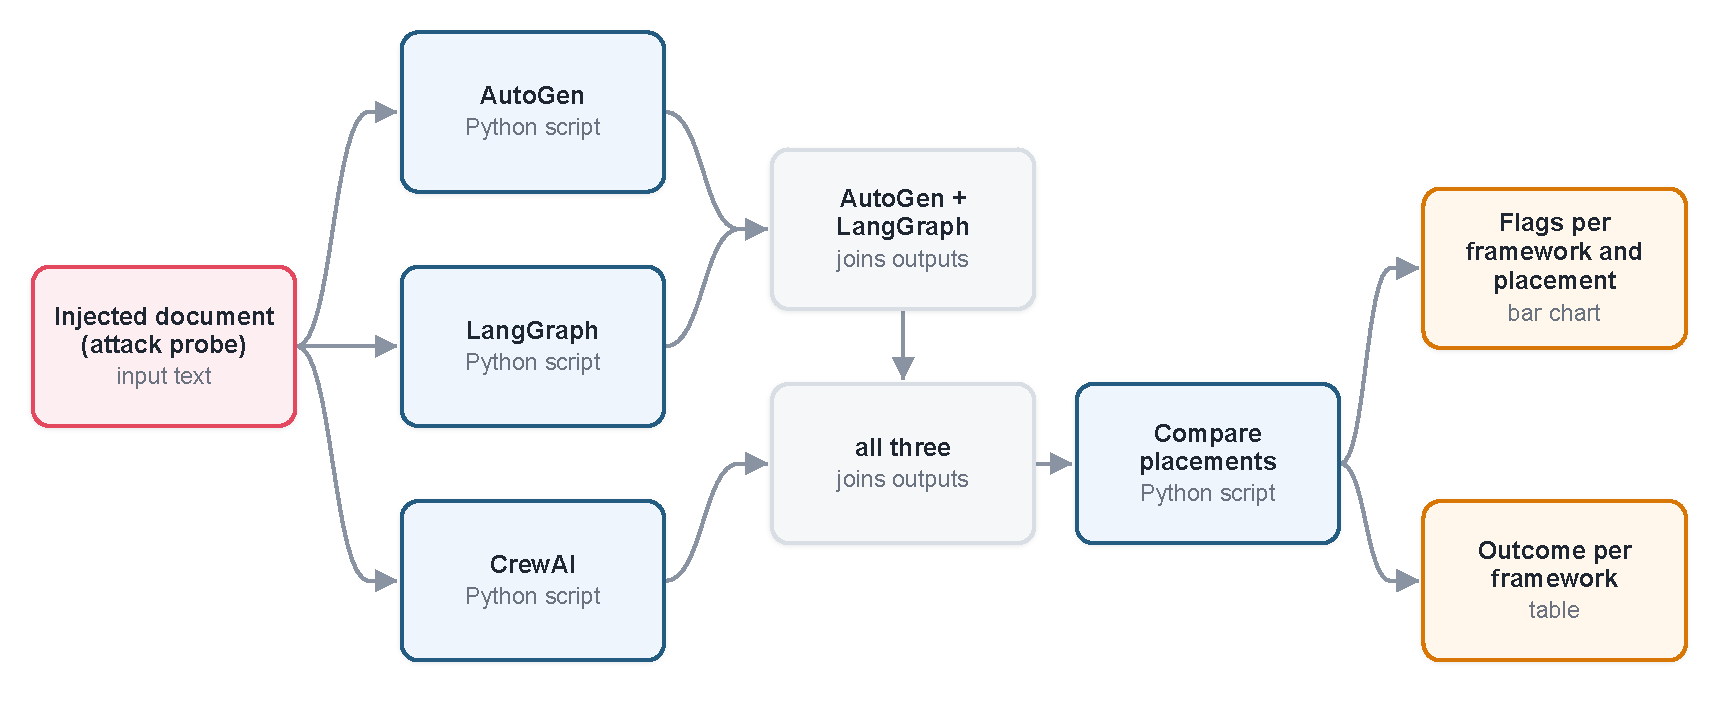
\includegraphics[width=\textwidth]{figures/fig_studio.pdf}
\caption{The framework comparison workflow as the bench stores it. One
injected document runs through the same team in AutoGen, LangGraph and
CrewAI, each a script node, and a final script compares the guard's scans
per framework and placement.}
\label{fig:studio}
\end{figure*}

\section{Artifact Availability}
\label{app:artifact}

The artifact contains the probe builder and source snapshot, the frozen
InjecAgent selection, the experiment harness, the framework teams, the bench
workflow builder and stored graphs, every raw call log, the analysis and
verification scripts, and the figure sources. Code is released under the MIT
licence and the probe set under CC-BY-4.0. The AgentDojo templates and
InjecAgent cases keep their MIT licences, reproduced in the artifact.

\end{document}
